\documentclass[authoryear,preprint,review,12pt]{elsarticle}

%
\usepackage{mysty}


\renewcommand{\baselinestretch}{1.5}
\oddsidemargin -5pt
\evensidemargin -5pt
\marginparwidth 25pt
\marginparsep 5pt
\topmargin -.50in
\textheight 8.8in
\textwidth 6.5in
\hoffset=0.2in
\begin{document}
	
	
	
	\begin{frontmatter}
		\author{Baofang Ke$^1$,    Weihua Zhao$^2$ and Lei Wang$^1$\footnote{Address for correspondence: Lei Wang, School of Statistics and Data Science \& LPMC, Nankai University. E-mail: lwangstat@nankai.edu.cn.} }
		\title{Projection-Based Inference for Low-Rank Matrix and Tensor Regression under Kronecker Covariance}
		\address{$^1$ School of Statistics and Data Science \& LPMC,
			Nankai University, Tianjin, 300071, P.R. China
			\\
			$^2$ School of Science, Nantong University, Nantong, 226019, P.R. China}
		\begin{abstract} 
			Low-rank matrix and tensor regression provides a parsimonious framework for modeling multi-way covariates, but valid inference for low-dimensional functionals of the coefficient object remains challenging. In particular, naive plug-in estimators are typically biased under low-rank regularization, and the bias can dominate stochastic fluctuation in high-dimensional regimes. The problem becomes more delicate when the design exhibits dependence, as is commonly captured by Kronecker-type covariance structures.
			
			We propose a projection-based inference framework for linear functionals of low-rank matrix and Tucker tensor coefficients. The key idea is to project a prespecified loading onto the tangent space of the low-rank manifold under the metric induced by the design covariance, thereby producing a covariance-weighted influence direction. Based on this projection-adjusted loading, we construct a one-step debiased estimator and develop feasible implementations using estimated covariance operators and sample splitting / cross-fitting.
			
			The framework yields a unified treatment of matrix and tensor regression. Under suitable regularity conditions, we establish asymptotic normality for both oracle and feasible estimators, which leads to valid Wald-type confidence intervals and hypothesis tests for target linear functionals. We further show that the resulting confidence intervals achieve the local geometric benchmark determined by the projection direction. For low-rank matrix regression under Kronecker covariance and for Tucker tensor regression under mode-wise Kronecker covariance, we derive explicit forms of the projection operator and practical inference algorithms.
			
			Simulation studies demonstrate that the proposed method achieves accurate coverage and competitive efficiency, with clear advantages under correlated designs. An application to resting-state EEG data illustrates how the proposed procedure turns scientifically meaningful matrix/tensor summaries into interpretable inferential targets with uncertainty quantification.
		\end{abstract}
		\begin{keyword}
			Low-rank structure; Projection-based inference; Matrix regression; Tensor regression; Cram\'er–Rao efficiency
		\end{keyword}
	\end{frontmatter}
	
	
	
	\section{Introduction}
	
	\subsection{Background and motivation}
	Low-rank matrix and tensor structures provide a parsimonious representation for multiway data and
	have become a central modeling device in modern statistics.
	In many applications, the covariate is naturally a matrix or a tensor and the response is scalar,
	leading to the linear model
	\begin{equation}\label{eq:model}
		y_i=\langle X_i,\Theta^\star\rangle+\varepsilon_i,\qquad i=1,\ldots,N,
	\end{equation}
	where $\Theta^\star$ is a low-rank matrix or a low Tucker-rank tensor.
	A substantial literature has focused on point estimation of $\Theta^\star$ under convex/nonconvex
	regularization (e.g., nuclear-norm penalization for matrices and low-rank factorizations for tensors)
	\citep{CandesRecht2009,NegahbanWainwright2011,KoldaBader2009,ZhouLiZhu2013}.
	
	In contrast, \emph{inference} for low-dimensional functionals of $\Theta^\star$ is considerably more
	challenging.
	In this paper, we study inference on linear functionals
	\begin{equation}\label{eq:target}
		\Delta_A \;=\;\langle A,\Theta^\star\rangle,
	\end{equation}
	where $A$ is a given loading matrix/tensor of scientific interest.
	Even when $\Delta_A$ is one-dimensional, naive plug-in estimators based on a low-rank estimator
	$\widehat\Theta$ can be severely biased due to shrinkage and rank constraints, and the bias typically
	dominates the stochastic fluctuation in high dimensions.
	Moreover, the dependence structure of $\mathrm{vec}(X_i)$ (often well described by Kronecker-type
	covariances) must be properly accounted for to obtain valid uncertainty quantification; see, e.g.,
	the matrix normal model and its variants \citep{Dutilleul1999}.
	These difficulties motivate a principled debiasing strategy that (i) respects the geometry induced
	by low-rank constraints and (ii) incorporates the covariance structure of the design.
	
	\subsection{Overview of the approach}
	Our methodology builds on a covariance-weighted projection principle.
	Viewing the low-rank parameter space as a smooth embedded manifold $\mathcal{M}$, the local geometry
	around $\Theta^\star$ is characterized by the tangent space $T_{\Theta^\star}\mathcal{M}$.
	We introduce a \emph{covariance-weighted projection} of the loading $A$ onto $T_{\Theta^\star}\mathcal{M}$
	under the metric induced by the design covariance
	$\Sigma=\mathrm{Cov}\{\mathrm{vec}(X_i)\}$.
	This yields a projection-adjusted loading $\Phi(A)$ which acts as an influence direction.
	Using $\Phi(A)$, we form a one-step estimator that corrects the plug-in bias by an empirical score-type
	term constructed from $(y_i,X_i)$.
	To ensure feasibility, we replace population quantities by sample analogues (including covariance and
	subspace estimators) and employ sample splitting / cross-fitting so that the estimated loading direction
	is (approximately) independent of the sample used in the debiasing step.
	
	\subsection{Contributions} 
	
	The main contributions of this paper are fourfold.
	
	First, we propose a covariance-weighted projection framework for inference on linear functionals in low-rank regression. The framework treats the low-rank parameter space as a smooth manifold and constructs a projection-adjusted loading by projecting the target loading onto the tangent space under the covariance-induced metric. This provides a unified inferential principle for both low-rank matrix regression and Tucker tensor regression.
	
	Second, based on the projection-adjusted loading, we develop a projection-based one-step debiasing estimator together with a transparent error decomposition. The decomposition separates the leading stochastic term from the effects of nuisance estimation, covariance approximation, and projection mismatch, and therefore directly clarifies the conditions required for valid feasible inference.
	
	Third, we derive concrete implementations under Kronecker-type dependence. For low-rank matrix regression with covariance \(\Sigma=\Sigma_q\otimes\Sigma_p\), we obtain explicit formulas for the covariance-weighted tangent-space projection and construct a feasible debiasing algorithm with Wald-type inference. For Tucker tensor regression with mode-wise Kronecker covariance, we develop the corresponding projection formulas and a feasible inference procedure based on mode-wise covariance estimation and HOSVD-type subspace recovery. In both cases, sample splitting or cross-fitting is used to decouple nuisance estimation from the debiasing step.
	
	Fourth, we establish asymptotic guarantees for both oracle and feasible procedures. In particular, we prove asymptotic normality for the proposed estimator and obtain valid confidence intervals and hypothesis tests for target linear functionals. We further show that the resulting confidence intervals achieve the local geometric benchmark induced by the projection direction. Simulation studies confirm accurate coverage and strong finite-sample performance, and a resting-state EEG application illustrates how the proposed framework enables uncertainty quantification for scientifically interpretable matrix and tensor summaries. 
	 
	
	\subsection{Organization}
	Section \ref{sec:framework} introduces the covariance-weighted projection operator, the projection-based one-step estimator, and its feasible implementation via sample splitting and cross-fitting.
	Sections~\ref{sec:matrix} and \ref{sec:tucker} specialize the framework to low-rank matrix regression under Kronecker covariance and Tucker tensor regression under mode-wise Kronecker covariance, respectively.
	Section~\ref{sec:inference} develops the asymptotic theory, including oracle and feasible normality results, verification of sufficient conditions in the matrix and tensor models, and local optimality of the resulting confidence intervals.
	Section~\ref{sec:simulation} reports simulation evidence on finite-sample estimation and inference.
	Section~\ref{sec:realdata} presents the EEG application.
	The paper concludes with a brief discussion, and the appendix collects the remaining technical proofs.
	
	\subsection{Notation}\label{sec:notation}
	For a positive integer $m$, let $[m]=\{1,\ldots,m\}$.
	Vectors are denoted by lowercase letters, matrices by bold uppercase letters (e.g., $\mathbf{X}$),
	and tensors by calligraphic letters (e.g., $\mathcal{X}$).
	For vectors $u,v\in\mathbb{R}^d$, $\langle u,v\rangle=u^\top v$.
	For matrices $A,B\in\mathbb{R}^{p\times q}$, the Frobenius inner product is
	$\langle A,B\rangle=\mathrm{tr}(A^\top B)$ and $\|A\|_F^2=\langle A,A\rangle$.
	For a tensor $\mathcal{A}$, $\|\mathcal{A}\|_F$ denotes its Frobenius norm.
	
	Let $\mathrm{vec}(\cdot)$ denote vectorization.
	For a third-order tensor $\mathcal{A}\in\mathbb{R}^{p_1\times p_2\times p_3}$,
	$\mathrm{Mat}_j(\mathcal{A})\in\mathbb{R}^{p_j\times (p_{j+1}p_{j+2})}$, $j=1,2,3$, denotes the mode-$j$
	matricization, where the indices are interpreted cyclically modulo $3$.
	The Kronecker product is denoted by $\otimes$.
	
	For a matrix $M$, $\|M\|$ is the operator norm and $\|M\|_*$ is the nuclear norm.
	For a symmetric matrix $S$, $\lambda_{\max}(S)$ and $\lambda_{\min}(S)$ denote its largest and
	smallest eigenvalues.
	For a positive semidefinite matrix $\Sigma$, define the $\Sigma$-weighted norms
	\[
	\|a\|_\Sigma^2 = a^\top \Sigma a,\qquad
	\|A\|_\Sigma^2 = \mathrm{vec}(A)^\top \Sigma\,\mathrm{vec}(A),
	\]
	whenever dimensions are compatible.
	For any tensor $\mA\in\mbr^{p_1\times p_2\times p_3}$, let $\mathbf{A}_j=\mathrm{Mat}_j(\mA)\in\mbr^{p_j\times (p_{j+1}p_{j+2})}$ for $j=1,2,3$. 
	
	Given a matrix $\bU\in\mathbb{R}^{p\times r}$, define the projection matrix as $\bP_{\bU}=\bU( \bU^{\top}\bU)^{-1}\bU^\top$  onto
	$\mathrm{col}(\bU)$ and $P_{\bU^\perp}=\mathbf{I}_p-\bP_{\bU}$. 
	Finally, $c,C>0$ denote generic constants whose values may change from line to line.
	Here, $\bar p=\max\{p_1,p_2,p_3\}, r=\max\{r_1,r_2,r_3\}$.
	Throughout the paper, bold uppercase letters (e.g., $\mathbf{X}$) denote matrices, 
	calligraphic letters (e.g., $\mathcal{X}$) denote tensors, 
	and standard letters denote scalars unless otherwise specified.
	% Bibliography (place at end of paper)
	% \bibliographystyle{plainnat}
	% \bibliography{refs}
	
	
	
	\section{A Covariance-Weighted Projection Framework}\label{sec:framework}
	
	In this section we present a unified inference framework that
	applies to both low-rank matrix regression and Tucker tensor regression.
	The key observation is that in both settings the parameter of interest
	lies on a smooth low-rank manifold, and valid inference for linear
	functionals can be achieved via a covariance-weighted projection
	onto the corresponding tangent space.
	
	\subsection{Model and Geometric Structure}
	
	Let $\Theta^\ast$ denote a low-rank parameter
	belonging to a smooth embedded manifold $\mathcal{M}$.
	We consider the regression model
	\begin{equation}\label{eq1}
		y_i = \langle \mathcal{X}_i, \Theta^\ast \rangle + \varepsilon_i,
		\quad i=1,\dots,N,
	\end{equation}
	where $\mathcal{X}_i$ is a matrix- or third-order tensor-valued covariate
	and $\varepsilon_i$ are independent mean-zero errors with variance $\sigma^2$. 
	Denote by
	\[
	\Sigma = \mathbb{E}\big[ \mathrm{vec}(\mathcal{X}_i)
	\mathrm{vec}(\mathcal{X}_i)^\top \big]
	\]
	the covariance operator of the vectorized covariates. 
	The projection principle developed in this section does not require any specific structure on the covariance operator $\Sigma$, 
	other than positive definiteness. 
	The Kronecker structure introduced later is imposed solely to obtain explicit expressions and simplified asymptotic analysis in structured low-rank models. 
	Let $T_{\Theta^\ast}\mathcal{M}$ denote the tangent space of $\mathcal{M}$
	at $\Theta^\ast$.
	Inference for linear functionals
	\[
	\Delta_A = \langle A, \Theta^\ast \rangle
	\]
	depends critically on how the loading object $A$
	interacts with the tangent space under the covariance-induced metric. 
	
	
	
	\subsection{Covariance-Weighted Projection Operator}
	
	Let $\mathcal{M}$ denote the low-rank manifold of interest, and let $T_{\Theta^\ast}\mathcal{M}$ be the tangent space of $\mathcal{M}$ at the true parameter $\Theta^\ast$. For a given object \( T \), we define the covariance-weighted projection operator $P_{\Sigma, \Theta^\ast}(T)$ as follows: 
	\begin{equation}
		P_{\Sigma, \Theta^\ast}(A) = \arg\min_{B \in T_{\Theta^\ast}\mathcal{M}} \| A - B \|_\Sigma^2.
		\label{eq:p}
	\end{equation}  
	This operator projects \( T \) onto the tangent space \( T_{\Theta^\ast}\mathcal{M} \) in a manner that minimizes the weighted squared distance according to the covariance structure. 
	Besides, we define the adjoint operator \( P_{\Sigma, \Theta^\ast}^\ast(A) \)  by
	\begin{equation}
		\mathrm{vec}(P_{\Sigma, \Theta^\ast}^\ast(A)) = \Sigma\mathrm{vec}(P_{\Sigma, \Theta^\ast}( \mathrm{vec}^{-1}(\Sigma^{-1}\mathrm{vec}(A)))).
		\label{eq:adjoint}
	\end{equation}
	This ensures that the operator \( P_{\Sigma, \Theta^\ast}(T) \) and its adjoint \( P_{\Sigma, \Theta^\ast}^\ast(A) \) satisfy the necessary conjugacy relation in the standard inner product space.  
	{ 
		\begin{pro}\label{pro:proj-basic}
			Let $P_{\Sigma,\Theta^\ast}$ be the $\Sigma$-weighted orthogonal projector onto the tangent space
			$T_{\Theta^\ast}\mathcal M$ defined in \eqref{eq:p} and $P_{\Sigma,\Theta^\ast}^\ast$ be its adjoint operator.
			For any matrices/tensors $A,B$ with compatible dimensions, it holds that: (a) for any $C\in T_{\Theta^\ast}\mathcal M,\, P_{\Sigma,\Theta^\ast}(C)=C;$ (b)  \( P_{\Sigma, \Theta^\ast}(A + B) =  P_{\Sigma, \Theta^\ast}(A)  + P_{\Sigma, \Theta^\ast}(B) \) and (c) \(\langle P_{\Sigma, \Theta^\ast}(A), B \rangle = \langle A, P_{\Sigma, \Theta^\ast}^\ast(B) \rangle\). 
		\end{pro} 
	}
	
	The operator   $P_{\Sigma,\Theta^\ast}$ identifies the tangent-space component of a loading under the covariance-induced metric, while its adjoint provides the standard-inner-product representation needed for debiasing. These objects lead directly to the projection-adjusted loading and the one-step estimator constructed in the next subsection.
	
	\subsection{Projection-Based One-Step Estimator}
	
	Let $\widehat{\Theta}$ denote a consistent initial estimator of $\Theta^\ast$ satisfying $\|\widehat{\Theta}-\Theta^\ast\|_F=o_p(1)$. 
	We construct the projection-based estimator
	\begin{equation}
		\widehat{\Delta}_A^{\mathrm{or}}
		=
		\langle A, P_{{\Sigma},{\Theta}^\ast}(\widehat{\Theta}) \rangle
		+
		\frac{1}{N} \sum_{i=1}^N \langle {\Phi}(A), \mathcal{X}_i \rangle
		\big(
		y_i - \langle \mathcal{X}_i, \widehat{\Theta} \rangle
		\big).
	\end{equation} 
	The error decomposition has the following form 
	\be\label{eq:err1}\widehat{\Delta}_A^{\mathrm{or}} - {\Delta}_A  = \underbrace{\frac{1}{N} \sum_{i=1}^N \langle {\Phi}(A), \mathcal{X}_i \rangle \varepsilon_i}_{\text{Stochastic error}}  + \underbrace{\big\langle P_{{\Sigma},{\Theta}^\ast}^\ast(A) -   \frac{1}{N} \sum_{i=1}^N \langle  {\Phi}(A), \mathcal{X}_i \rangle     \mathcal{X}_i,  \widehat{\Theta} - \Theta^\ast\big\rangle}_{\text{Remainder term}}.\ee
	The first term in the RHS  is the stochastic error, while the second term denotes the remaining bias.
	Define the projection-adjusted loading
	\[
	\mathrm{vec}({\Phi}(A)) = \Sigma \mathrm{vec}(P_{{\Sigma},{\Theta}^\ast}^\ast(A)),
	\]
	such that
	\[
	{\Phi}(A) =  P_{\Sigma, \Theta^\ast}( \mathrm{vec}^{-1}(\Sigma^{-1}\mathrm{vec}(A))).
	\]
	With such projection-adjusted loading, we can prove that, when $N$ is large enough, the remainder term satisfies that
	$$\mbe[ \langle  {\Phi}(A), \mathcal{X}_i \rangle     \mathcal{X}_i] =P_{{\Sigma},{\Theta}^\ast}^\ast(A),$$
	and thus can be asymptotic negligible and the asymptotic variance of $\widehat{\Delta}_A^{\Phi}$ is 
	\[
	\mathrm{Var}\big( \varepsilon_i\langle \Phi(A), \mathcal{X}_i \rangle \big)
	= \sigma^2 
	\|\Phi(A)\|_\Sigma^2.
	\]
	
	\subsection{Feasible Implementations}
	
	Throughout the paper, \(N\) denotes the total sample size. Under balanced sample splitting, we write \(N=2n\) and \(|\mD_1|=|\mD_2|=n\), where \(n\) is used only for half-sample nuisance estimation.
	
	The estimator defined above assumes access to the population  projection-adjusted loading ${\Phi}(A)$
	and  the true tangent space $\mathcal{M}$.  
	This serves as a conceptual benchmark for deriving the asymptotic variance and efficiency bound.
	In practical implementations, we construct  the feasible projection-adjusted loading
	\[
	\widehat{\Phi}(A)
	=  P_{\widehat{\Sigma},\widehat{\Theta}}( \mathrm{vec}^{-1}(\widehat\Sigma^{-1}\mathrm{vec}(A))),
	\]
	where $\widehat{\Sigma}$ is the empirical covariance operator.  
	And the feasible projection-based estimator is defined then by 
	\begin{equation}
		\widehat{\Delta}_A^{\mathrm{fe}}
		=
		\langle A, P_{\widehat{\Sigma},\widehat{\Theta}}(\widehat{\Theta}) \rangle
		+
		\frac{1}{N}
		\sum_{i=1}^N
		\langle \widehat{\Phi}(A), \mathcal{X}_i \rangle
		\big(
		y_i - \langle \mathcal{X}_i, \widehat{\Theta} \rangle
		\big).
	\end{equation} 
	\paragraph{Independence via sample splitting/cross-fitting}
	Throughout the paper, the asymptotic normality results are established under the principle that
	the nuisance quantities (e.g., $\widehat\Theta$ and covariance/subspace estimates) used to construct
	the debiasing direction are computed from data that are independent of the sample used in the
	one-step correction. This can be ensured by sample splitting, and can be relaxed via cross-fitting.
	
	The error decomposition then has the following form
	\begin{equation}
		\widehat{\Delta}_A^{\mathrm{fe}} - {\Delta}_A  = \underbrace{\frac{1}{N} \sum_{i=1}^N \langle \widehat{\Phi}(A), \mathcal{X}_i \rangle \varepsilon_i}_{\text{Stochastic error}}
		+ \underbrace{\big\langle P_{\widehat{\Sigma},\widehat{\Theta}}^\ast(A) -   \frac{1}{N} \sum_{i=1}^N \langle  \widehat{\Phi}(A), \mathcal{X}_i \rangle     \mathcal{X}_i,  \widehat{\Theta} - \Theta^\ast\big\rangle}_{\text{Remainder term}} + \underbrace{\langle   P_{\widehat{\Sigma},\widehat{\Theta}}^\ast(A) - A, \Theta^\ast\rangle}_{\text{Additional term}}.
		\label{eq:feasible_err}
	\end{equation}
	The asymptotic normality property of the stochastic error term is straightforward when $\widehat\Phi(A)$ and $\{\varepsilon_i, \mathcal{X}_i\}_i$'s are independent. This can be achieved via sample splitting technique. Furthermore, when $\widehat\Sigma \stackrel{p}{\rightarrow} \Sigma$,
	$$\mbe[ \langle  \widehat{\Phi}(A), \mathcal{X}_i \rangle     \mathcal{X}_i] \approx P_{\widehat{\Sigma},\widehat{\Theta}}^\ast(A),$$
	which leads to a negligible remainder term. 
	Compared with \eqref{eq:err1}, there exists an additional term introduced by the estimate error of $P_{\widehat{\Sigma},\widehat{\Theta}}$. In fact, let $\widetilde A = \mathrm{vec}^{-1}(\widehat\Sigma^{-1}\mathrm{vec}(A))$, then
	\[ \langle P_{\widehat{\Sigma},\widehat{\Theta}}^\ast(A) - A, \Theta^\ast\rangle= \langle P_{\widehat\Sigma, \widehat\Theta }(\widetilde A) - \widetilde A, \Theta^\ast\rangle_{\widehat\Sigma} = \langle P_{\widehat\Sigma, \widehat\Theta }(\widetilde A) - \widetilde A, P_{\widehat\Sigma, \widehat\Theta }^{\perp}(\Theta^\ast) \rangle_{\widehat\Sigma},\]
	where the last equality holds since $\langle P_{\widehat\Sigma, \widehat\Theta }(\widetilde A) - \widetilde A, P_{\widehat\Sigma, \widehat\Theta } (\Theta^\ast) \rangle_{\widehat\Sigma}  = 0.$ And it can be expected that $P_{\widehat\Sigma, \widehat\Theta }^{\perp}(\Theta^\ast)$ is small term by the consistency of $\widehat\Theta$.
	
	
	
	
	\section{Application to Low-Rank Matrix Regression}\label{sec:matrix}
	
	\subsection{Model specification and geometric objects}
	In the matrix case, we specialize $\mathcal{X}_i$ to $\mathbf{X}_i \in \mathbb{R}^{p\times q}$, $\Theta^\ast$ to $\bTheta^\ast \in \mathbb{R}^{p\times q}$  and $\mathcal{M}$ being the smooth manifold of rank-$r$ matrices such that  $\bTheta^\ast = \bU^\ast \bV^{\ast\top}$ for some $\bU^\ast\in\mbr^{p\times r}, \bV^\ast\in\mbr^{q\times r}$. Consider the trace regression model
	\begin{equation}
		y_i = \langle \mathbf{X}_i, \bTheta^\ast \rangle + \varepsilon_i, 
		\quad i = 1,\dots,N.
	\end{equation}
	In this section, we focus on the estimation and inference for the linear function  $\Delta_{\bA}=\langle \bA,\bTheta^\ast\rangle$.
	
	To derive explicit formulas for the covariance-weighted projection operator 
	and to facilitate dimension-dependent asymptotic analysis, 
	we assume that the covariance matrix admits a Kronecker product structure,
	\[
	\bSigma = \bSigma_q \otimes \bSigma_p,
	\] 
	where $\bSigma_p\in\mbr^{p\times p}$ and $\bSigma_q\in\mbr^{q\times q}$ are both positive matrices.  
	We specialize the abstract operators 
	$P_{\Sigma,\Theta^\ast}$ and $P_{\Sigma,\Theta^\ast}^\ast$ 
	to the rank-$r$ matrix manifold. 
	To avoid ambiguity, we denote the corresponding operators by
	$P_{\bSigma,\bTheta^\ast}$ and 
	$P_{\bSigma,\bTheta^\ast}^\ast$.  
	We next provide explicit expressions of $P_{\bSigma,\bTheta^\ast}$ and 
	$P_{\bSigma,\bTheta^\ast}^\ast$
	under the Kronecker covariance model:
	\begin{equation*}
		\begin{aligned}
			P_{\bSigma,\mathbf\Theta^\ast}(\mathbf A)
			&=
			\mathbf P_{\mathbf U^\ast}^{\mathbf \Sigma_p}
			\,\mathbf \Sigma_p \mathbf A \mathbf \Sigma_q\,
			\mathbf P_{\mathbf V^\ast}^{\mathbf \Sigma_q} 
			+
			\mathbf P_{\mathbf U^\ast}^{\mathbf \Sigma_p}
			\,\mathbf \Sigma_p \mathbf A\,
			(\mathbf I_q - \mathbf \Sigma_q \mathbf P_{\mathbf V^\ast}^{\mathbf \Sigma_q}) 
			+
			(\mathbf I_p - \mathbf P_{\mathbf U^\ast}^{\mathbf \Sigma_p}\mathbf \Sigma_p)
			\,\mathbf A \mathbf \Sigma_q\,
			\mathbf P_{\mathbf V^\ast}^{\mathbf \Sigma_q},
			\\[1.2ex]
			P_{\bSigma,\mathbf\Theta^\ast}^{\ast}(\mathbf A)
			&=
			\mathbf \Sigma_p \mathbf P_{\mathbf U^\ast}^{\mathbf \Sigma_p}
			\,\mathbf A\,
			\mathbf P_{\mathbf V^\ast}^{\mathbf \Sigma_q}\mathbf \Sigma_q 
			+
			\mathbf \Sigma_p \mathbf P_{\mathbf U^\ast}^{\mathbf \Sigma_p}
			\,\mathbf A\,
			(\mathbf I_q - \mathbf P_{\mathbf V^\ast}^{\mathbf \Sigma_q}\mathbf \Sigma_q) 
			+
			(\mathbf I_p - \mathbf \Sigma_p \mathbf P_{\mathbf U^\ast}^{\mathbf \Sigma_p})
			\,\mathbf A\,
			\mathbf P_{\mathbf V^\ast}^{\mathbf \Sigma_q}\mathbf \Sigma_q .
		\end{aligned}
	\end{equation*}
	where
	\[
	\mathbf P_{\mathbf U^\ast}^{\mathbf \Sigma_p}
	=
	\mathbf U^\ast(\mathbf U^{\ast\top} \mathbf \Sigma_p \mathbf U^\ast)^{-1}\mathbf U^{\ast\top}
	\in \mathbb R^{p\times p},
	\qquad
	\mathbf P_{\mathbf V^\ast}^{\mathbf \Sigma_q}
	=
	\mathbf V^\ast(\mathbf V^{\ast\top} \mathbf \Sigma_q \mathbf V^\ast)^{-1}\mathbf V^{\ast\top}
	\in \mathbb R^{q\times q}.
	\]
	Then the oracle projection-based estimate for the linear functional
	$\Delta_{\bA}$ is constructed as followed.  
	Define 
	\begin{equation}
		\Phi(\mathbf A)
		=
		P_{\bSigma,\mathbf{\Theta}^\ast}
		\bigl(\mathbf \Sigma_p^{-1}\mathbf A \mathbf \Sigma_q^{-1}\bigr)
		=
		\mathbf P_{\mathbf U^\ast}^{\mathbf \Sigma_p}
		\,\mathbf A\,
		\mathbf P_{\mathbf V^\ast}^{\mathbf \Sigma_q} 
		+
		\mathbf P_{\mathbf U^\ast}^{\mathbf \Sigma_p}
		\,\mathbf A\,
		\bigl(\mathbf \Sigma_q^{-1} - \mathbf P_{\mathbf V^\ast}^{\mathbf \Sigma_q}\bigr) 
		+
		\bigl(\mathbf \Sigma_p^{-1} - \mathbf P_{\mathbf U^\ast}^{\mathbf \Sigma_p}\bigr)
		\,\mathbf A\,
		\mathbf P_{\mathbf V^\ast}^{\mathbf \Sigma_q}.
		\label{eq:phi_mat}
	\end{equation}
	The oracle projection-based estimator is
	\begin{equation}
		\widehat\Delta_\bA^{\,\mathrm{or}}
		=
		\langle \bA, P_{\bSigma,\mathbf{\Theta}^\ast}(\widehat{\bTheta})\rangle
		+
		\frac{1}{N}\sum_{i=1}^N
		\langle \Phi(\bA),\mathbf X_i\rangle
		\bigl(y_i-\langle \mathbf X_i,\widehat\bTheta\rangle\bigr).
		\label{eq:oracle-matrix}
	\end{equation}
	
	
	
	\subsection{Feasible implementation: nuisance estimation and debiasing}
	\label{sec:mat_nuisance}
	To ensure the independency between $\widehat\bTheta, \widehat\Phi$ and the dominated term, we use a sample splitting technique. 
	Without loss of generality,  we assume $N=2n$ samples $\mD = \{(y_i, \bX_i)\}_{i=1}^{2n}$, divided into two disjoint subsets  $\mD_1 = \{(y_i, \bX_i)\}_{i=1}^{n}$ and $\mD_2 = \{(y_i, \bX_i)\}_{i=n+1}^{2n}$. 
	
	Without of loss generality, we describe the  estimate $\wh\Delta_{\bA}^{(1)}$, which is estimated based on $\mD_1$. And the nuisances therein are estimated by the second half of the sample $\mD_2$. Define the following empirical quantities
	\be\label{eq:cov}\widetilde \bSigma_p = \frac{1}{|\mD_2|}\sum_{i\in\mD_2} \bX_i\bX_i^{\top},\quad  \widetilde\bSigma_q  = \frac{1}{|\mD_2|}\sum_{i\in\mD_2} \bX_i^{\top}\bX_i,\quad  b_n =  \frac{1}{|\mD_2|}\sum_{i\in\mD_2} \|\bX_i\|_F^2 .\ee
	The normalized column and row covariance estimates are then given by  
	\be\label{eq:cov2}\wh\bSigma_p = \frac{1}{\sqrt{b_n}}\wt \bSigma_p ,\quad \wh\bSigma_q = \frac{1}{\sqrt{b_n}} \wt \bSigma_q.\ee
	Let  $\wh\bTheta$ be the initial estimate based on $\mD_2$ and $\wh\bU \in \mathbb{R}^{p \times r}$ and $\wh\bV \in \mathbb{R}^{q \times r}$ denote the top-$r$ left and right singular vectors of $\wh\bTheta$, respectively. Then the estimated generalized projection operators $\bP_{\bU^\ast}^{\bSigma_p}$ and $\bP_{\bV^\ast}^{\bSigma_q}$  can be approximated by $\bP_{\wh\bU}^{\wh\bSigma_p}$ and $\bP_{\wh\bV}^{\wh\bSigma_q}$, such that $	P_{\bSigma,\mathbf\Theta^\ast}(\mathbf A)$ can be estimated by $	P_{\wh\bSigma,\wh\bTheta_r}(\mathbf A)$. 
	Besides, we estimate the  projection-adjusted loading  $\widehat\Phi(\bA) =    P_{\widehat\bSigma,\widehat\bTheta_r}(\widehat\bSigma_p^{-1}\bA \widehat\bSigma_q^{-1})$ with $\wh\bTheta_r$ being the rank-$r$ truncated matrix of $\wh\bTheta$.
	The feasible projection-base one-step estimator is
	\begin{equation} 
		\widehat\Delta_\bA^{(1)}
		=
		\langle \bA, P_{\widehat\bSigma,\widehat\bTheta_r}(\widehat\bTheta)\rangle
		+
		\frac{1}{n}\sum_{i=1}^n
		\langle \widehat\Phi(\bA),\mathbf X_i\rangle
		\bigl(y_i-\langle \mathbf X_i,\widehat\bTheta\rangle\bigr).
		\label{eq:feasible-matrix}
	\end{equation} 
	We repeat the same procedure by exchanging the roles of $\mD_1$ and $\mD_2$, obtaining a second estimate  $\wh\Delta_{\bA}^{(2)}$. The final practical estimator is then defined as the average 
	\be\label{eq:final} \wh\Delta_{\bA}  = \frac{1}{2}(\wh\Delta_{\bA}^{(1)} + \wh\Delta_{\bA}^{(2)} ).\ee 
	The algorithm is summarized as the following.  
	\begin{algorithm}
		\caption{Feasible Projection-base One Step Estimate}
		\label{alg:debias}
		\begin{algorithmic}[1]
			\Require Independent datasets $\mD_1$ and $\mD_2$; initial estimators $\wh\bTheta^{(1)}$ and $\wh\bTheta^{(2)}$ are computed from $\mD_1$ and $\mD_2$, respectively.
			\Ensure Debiased estimator $\wh\Delta_{\bA}$
			
			\State Extract the top-$r$ eigenvectors of $\wh\bTheta^{(2)}$, denoted by $\wh\bU$ and $\wh\bV$. \label{step:eigen}
			\State Compute covariance estimators $\wh\bSigma_p$ and $\wh\bSigma_q$ from $\mD_2$ according to \eqref{eq:cov}--\eqref{eq:cov2}.
			\State Compute  $\widehat\Phi(\bA) =    P_{\widehat\bSigma,\widehat\bTheta_r}(\widehat\bSigma_p^{-1}\bA \widehat\bSigma_q^{-1})$. 
			\State Compute $\wh\Delta_{\bA}^{(1)}$ via \eqref{eq:feasible-matrix}. \label{step:first_estimate}
			\State Repeat Steps \ref{step:eigen}–\ref{step:first_estimate} by switching the roles of $\mD_1$ and $\mD_2$ and obtain $\wh\Delta_{\bA}^{(2)}$.
			\State \Return Final estimator: $\wh\Delta_{\bA} =  (\wh\Delta_{\bA}^{(1)} + \wh\Delta_{\bA}^{(2)})/2$.
		\end{algorithmic}
	\end{algorithm}
	
	\subsection{Hypothesis testing and confidence intervals}
	\label{sec:matrix_inf}
	In this section we focus  on the statistical inference procedure for $\Delta_{\bA}$. We will prove in  Corollary \ref{cor:asym_normal_fe} that, the feasible estimate defined in  \eqref{eq:final} has the asymptotic normality that
	$$\sqrt{2n}V^{-1/2}(\wh\Delta_{\bA} -\Delta_{\bA} )\stackrel{d}{\rightarrow} N(0,1),$$
	with $V = \sigma^2 \|\Phi(\bA)\|_{\bSigma}^2 = \sigma^2 \|\bSigma_p^{1/2}\Phi(\bA)\bSigma_q^{1/2}\|_F^2$. 
	The estimator for $\sigma^2$ is proposed by
	\begin{equation}
		\wh\sigma^2 = \frac{1}{2n}\sum_{i \in \mD_1}(y_i  - \langle\bX_i, \wh\bTheta^{(2)}\rangle)^2 +  \frac{1}{2n}\sum_{i \in \mD_2}(y_i  - \langle\bX_i, \wh\bTheta^{(1)}\rangle)^2.
		\label{eq:matrix_vhat}
	\end{equation}
	And we estimate $V$ by
	\begin{equation}
		\wh V = \hat\sigma^2 \|\wh\bSigma_p^{1/2} \Phi(\bA)\wh\bSigma_q^{1/2}\|_F^2.
		\label{eq:matrix_v}
	\end{equation}
	Furthermore, the $(1-\alpha)$-level confidence interval for $\Delta_{\bA}$ is constructed as
	$$\text{CI}_{\alpha}(\bA, \mD) = \Big[\wh\Delta_{\bA} - z_{\alpha/2}\frac{ \wh V^{1/2}}{\sqrt{2n}},\quad \wh\Delta_{\bA} + z_{\alpha/2}\frac{ \wh V^{1/2}}{\sqrt{2n}}\Big].$$
	
	\section{Application to Tucker Tensor Regression}
	\label{sec:tucker}
	
This section specializes the covariance-weighted projection framework in Section~\ref{sec:framework}
	to third-order Tucker low-rank tensor regression. Although the Tucker geometry is more involved than the matrix case,
	the inference principle remains the same: we debias the plug-in estimator of a linear functional by
	projecting an appropriate loading tensor onto the tangent space under the covariance-induced metric.
	
	\subsection{Model specification and Kronecker covariance}
	\label{subsec:tucker:model}
	
	Let $\mathcal{X}_i \in \mathbb{R}^{p_1\times p_2\times p_3}$ be third-order tensor-valued covariates and consider
	the third-order tensor linear regression model
	\begin{equation}
		y_i \;=\; \langle \mathcal{X}_i, \mT^\ast \rangle + \varepsilon_i,
		\qquad i=1,\ldots,N,
		\label{eq:tucker:model}
	\end{equation}
	where $\varepsilon_i$ are independent mean-zero errors with variance $\sigma^2$ and independent of
	$\{\mathcal{X}_i\}_{i=1}^N$.
	Given a loading tensor $\mA\in\mathbb{R}^{p_1\times p_2\times p_3}$, our target is inference for
	the linear functional $\Delta_{\mA} \;=\; \langle \mA, \mT^\ast \rangle.$
	
	To obtain explicit operator expressions and simplify the subsequent analysis, we assume a Kronecker
	covariance structure on the vectorized covariate:
	\begin{equation}
		\bSigma \;=\; \mathrm{Cov}(\mathrm{vec}(\mathcal{X}_i))
		\;=\; \bSigma_{p_3}\otimes \bSigma_{p_2}\otimes \bSigma_{p_1},
		\label{eq:tucker:kronecker}
	\end{equation}
	where each $\bSigma_{p_j}\in\mathbb{R}^{p_j\times p_j}$ is positive definite.
	
	\subsection{Tucker manifold and covariance-weighted estimators}
	\label{subsec:tucker:manifold} 
	Assume $\mT^\ast$ has Tucker multilinear rank $(r_1,r_2,r_3)$ and admits the decomposition
	\[
	\mT^\ast \;=\; \mathcal{G}^\ast \times_1 \mathbf{U}_1^\ast \times_2 \mathbf{U}_2^\ast \times_3 \mathbf{U}_3^\ast,
	\]
	where the core tensor $\mathcal{G}^\ast \in \mathbb{R}^{r_1\times r_2\times r_3}$ and
	$\mathbf{U}_j^\ast\in \mathbb{R}^{p_j\times r_j}$ has orthonormal columns for $j=1,2,3$.
	Let $\mathcal{M}_{\mathbf{r}}$ denote the smooth manifold of tensors with Tucker rank $\mathbf{r}=(r_1,r_2,r_3)$.
	At a point $\mT=\mathcal{G}\times_1 \mathbf{U}_1\times_2 \mathbf{U}_2\times_3 \mathbf{U}_3 \in \mathcal{M}_{\mathbf{r}}$,
	the tangent space $T_{\mathcal{M}}\mathcal{M}_{\mathbf{r}}$ can be parameterized as
	\begin{equation}
		T_{\mathcal{M}}\mathcal{M}_{\mathbf{r}}
		=
		\Bigl\{
		\dot{\mathcal{G}}\times_1 \mathbf{U}_1\times_2 \mathbf{U}_2\times_3 \mathbf{U}_3
		+
		\sum_{j=1}^3
		\mathcal{G}\times_j \dot{\mathbf{U}}_j \times_{k\neq j}\mathbf{U}_k
		\;:\;
		\dot{\mathbf{U}}_j^\top \mathbf{U}_j=\mathbf{0}
		\Bigr\}.
		\label{eq:tucker:tangent}
	\end{equation} 
	Let $\mathbf{P}_{\mathbf{U}_j^\ast}^{\bSigma_{p_j}}
	=
	\mathbf{U}_j^\ast \bigl((\mathbf{U}_j^\ast)^\top \bSigma_{p_j}\mathbf{U}_j^\ast\bigr)^{-1}(\mathbf{U}_j^\ast)^\top$
	be the generalized projection for $j=1,2,3$. 
	Under \eqref{eq:tucker:kronecker}, the abstract operator $P_{\Sigma,\Theta^\ast}$ in Section~\ref{sec:framework}
	admits the following explicit form on the Tucker manifold:
	for any $\mathcal{A}\in\mathbb{R}^{p_1\times p_2\times p_3}$,
	\begin{align}
		P_{\bSigma,\mT^\ast}(\mathcal{A})
		&=
		\mathcal{A}\times_1 \mathbf{P}_{\mathbf{U}_1^\ast}^{\bSigma_{p_1}}\bSigma_{p_1}
		\times_2 \mathbf{P}_{\mathbf{U}_2^\ast}^{\bSigma_{p_2}}\bSigma_{p_2}
		\times_3 \mathbf{P}_{\mathbf{U}_3^\ast}^{\bSigma_{p_3}}\bSigma_{p_3}
		\;+\;
		\sum_{j=1}^3 \mathcal{G}^\ast \times_{k\neq j}\mathbf{U}_k^\ast \times_j \mathbf{W}_{j1},
		\label{eq:tucker:P}
		\\
		P_{\bSigma,\mT^\ast}^{\ast}(\mathcal{A})
		&=
		\mathcal{A}\times_1 \bSigma_{p_1}\mathbf{P}_{\mathbf{U}_1^\ast}^{\Sigma_{p_1}}
		\times_2 \bSigma_{p_2}\mathbf{P}_{\mathbf{U}_2^\ast}^{\bSigma_{p_2}}
		\times_3 \bSigma_{p_3}\mathbf{P}_{\mathbf{U}_3^\ast}^{\bSigma_{p_3}}
		\;+\;
		\sum_{j=1}^3 \mathcal{G}^\ast \times_{k\neq j}\bSigma_{p_k}\mathbf{U}_k^\ast \times_j \mathbf{W}_{j2},
		\label{eq:tucker:Padj}
	\end{align}
	where $\mathbf{W}_{j1}$ and $\mathbf{W}_{j2}$ are defined as
	\begin{align*}
		\mathbf{W}_{j1}
		&=
		\bigl(\mathbf{I}_{p_j}-\mathbf{P}_{\mathbf{U}_j^\ast}^{\bSigma_{p_j}}\bSigma_{p_j}\bigr)\,
		\bA_j\,
		\Bigl(\bigotimes_{k\neq j}\bSigma_{p_k}\mathbf{U}_k^\ast\Bigr)\,
		(\mathbf{G}_j^\ast)^\top\,
		\Bigl(\mathbf{G}_j^\ast \Bigl[\bigotimes_{k\neq j}(\mathbf{U}_k^\ast)^\top\bSigma_{p_k}\mathbf{U}_k^\ast\Bigr](\mathbf{G}_j^\ast)^\top\Bigr)^{-1},
		\\
		\mathbf{W}_{j2} 
		&=
		\bigl(\mathbf{I}_{p_j}-\bSigma_{p_j}\mathbf{P}_{\mathbf{U}_j^\ast}^{\bSigma_{p_j}}\bigr)\,
		\bA_j\,
		\Bigl(\bigotimes_{k\neq j}\mathbf{U}_k^\ast\Bigr)\,
		(\mathbf{G}_j^\ast)^\top\,
		\Bigl(\mathbf{G}_j^\ast \Bigl[\bigotimes_{k\neq j}(\mathbf{U}_k^\ast)^\top\bSigma_{p_k}\mathbf{U}_k^\ast\Bigr](\mathbf{G}_j^\ast)^\top\Bigr)^{-1},
	\end{align*}
	and $\mathbf{G}_j^\ast$ denotes the mode-$j$ matricization of $\mathcal{G}^\ast$.
	
	
	
	\paragraph{Oracle estimator}
	Define the oracle projection-adjusted loading
	\begin{equation}
		\Phi(\mathcal{A})
		=\;
		P_{\bSigma,\mT^\ast}\!\bigl(\mathrm{vec}^{-1}(\bSigma^{-1}\mathrm{vec}(\mathcal{A}))\bigr)  
		=
		\mathcal{A}\times_1 \mathbf{P}_{\mathbf{U}_1^\ast}^{\bSigma_{p_1}} 
		\times_2 \mathbf{P}_{\mathbf{U}_2^\ast}^{\bSigma_{p_2}} 
		\times_3 \mathbf{P}_{\mathbf{U}_3^\ast}^{\bSigma_{p_3}} 
		\;+\;
		\sum_{j=1}^3 \mathcal{G}^\ast \times_{k\neq j}\mathbf{U}_k^\ast \times_j \mathbf{W}_{j3},
		\label{eq:tucker:Phi-oracle}
	\end{equation}
	with 
	\[\mathbf{W}_{j3}=
	\bigl(\mathbf{I}_{p_j}-\mathbf{P}_{\mathbf{U}_j^\ast}^{\bSigma_{p_j}} \bigr)\,
	\bA_j\,
	\Bigl(\bigotimes_{k\neq j} \mathbf{U}_k^\ast\Bigr)\,
	(\mathbf{G}_j^\ast)^\top\,
	\Bigl(\mathbf{G}_j^\ast \Bigl[\bigotimes_{k\neq j}(\mathbf{U}_k^\ast)^\top\bSigma_{p_k}\mathbf{U}_k^\ast\Bigr](\mathbf{G}_j^\ast)^\top\Bigr)^{-1},
	\]
	Then the oracle one-step estimator for $\Delta_{\mA}$ takes the same form as in Section~\ref{sec:framework}:
	\begin{equation}
		\widehat{\Delta}^{\mathrm{or}}_{\mA}
		\;=\;
		\bigl\langle \mA,\, P_{\bSigma,\mT^\ast}(\wh\mT) \bigr\rangle
		\;+\;
		\frac{1}{N}\sum_{i=1}^N
		\bigl\langle \Phi(\mA),\, \mathcal{X}_i \bigr\rangle
		\bigl(y_i-\langle \mathcal{X}_i, \wh\mT\rangle\bigr),
		\label{eq:tucker:oracle-est}
	\end{equation}
	where $\wh\mT$ is any   consistent initial estimator of $\mT^\ast$.
	
	
	\subsection{Feasible implementation: nuisance estimation and debiasing}\label{sec:feasible}
	Similar with Section \ref{sec:mat_nuisance}, we adopt a sample-splitting strategy to ensure that the estimated loading $\wh\Phi(\mA)$ is independent of the
	bias-correction step. Denote $\mD_1 = \{ (y_i, \mX_i)\}_{i=1}^n,\ \mD_2 = \{ (y_i, \mX_i)\}_{i=n+1}^{2n}$ and $\mD = \mD_1\cup\mD_2$. 
	Without of loss generality, we describe the feasible projection-based estimate $\wh\Delta_{\mA}^{(1)}$ based on $\mD_1$. And the nuisances therein are estimated by the independent dataset $\mD_2$. 
	Specifically, we define 
	\be\label{eq:cov3}\wt\bSigma_{p_j} = \frac{1}{|\mD_2|}\sum_{i\in\mD_2}  \text{Mat}_j(\mX_i)^{\otimes 2},\ j=1,2,3,\quad b_n =  \frac{1}{|\mD_2|}\sum_{i\in\mD_2} \|\mX_i\|_F^2. \ee
	Then the normalized covariance estimates for $\bSigma_j$'s are given by
	\be\label{eq:cov4}\wh\bSigma_{p_j} = \frac{1}{b_n^{2/3}}\wt\bSigma_{p_j}, \quad j=1,2,3.\ee
	Thus, $	\bSigma$ is estimated by
	\begin{equation}
		\wh\bSigma = \wh\bSigma_{p_3} \otimes \wh\bSigma_{p_2} \otimes \wh\bSigma_{p_1}.
		\label{eq:deign_tensor}
	\end{equation}
	
	Let $\wh\mT$ be estimated based on $\mD_2$ and $\wh\mT_{\br}$ be a consistent Tucker-rank $(r_1, r_2, r_3)$ tensor with $\wh\mT_{\br} = \wh\mG\times_1 \wh\bU_1 \times_2 \wh\bU_2  \times_3 \wh\bU_3$, where $\wh\mG\in\mbr^{r_1\times r_2\times r_3}$ and $\wh\bU_j\in\mbr^{p_j\times r_j}$ for $j=1,2,3$.  Such low Tucker-rank tensor can be obtained via HOSVD algorithm. 
	And the estimated generalized projection operators $P_{\bSigma,\mT^\ast}(\mathcal{A})$ in \eqref{eq:tucker:P} can be approximated by $P_{\wh\bSigma, \wh\mT_{\br}}(\mathcal{A})$. Besides,  the projection-adjusted loading $\Phi(\mA)$ is estimated by $\wh \Phi(\mA) = P_{\wh\bSigma, \wh\mT_{\br}}\!\bigl(\mathrm{vec}^{-1}(\wh \bSigma^{-1}\mathrm{vec}(\mathcal{A}))\bigr)$. The feasible projection-based estimator is then defined as
	\begin{equation}
		\widehat{\Delta}^{(1)}_{\mA}
		\;=\;
		\bigl\langle \mA,\, P_{\wh\bSigma, \wh\mT_{\br}}(\wh\mT) \bigr\rangle
		\;+\;
		\frac{1}{|\mD_1|}\sum_{i\in \mD_1}
		\langle \wh\Phi(\mA),\, \mathcal{X}_i \rangle
		(y_i-\langle \mathcal{X}_i, \wh\mT\rangle).
		\label{eq:tensor_feasible}
	\end{equation} 
	Repeat the same procedure by exchanging the roles of $\mD_1$ and $\mD_2$ to obtain $\widehat{\Delta}^{(2)}_{\mA}$. And the final feasible projection-based estimate is defined as
	\begin{equation}
		\widehat{\Delta}_{\mA} = \frac{1}{2} ( \widehat{\Delta}_{\mA}^{(1)} + \widehat{\Delta}_{\mA}^{(2)}).
		\label{eq:final_tensor}
	\end{equation}
	The algorithm is summarized in Algorithm \ref{alg:tensor_debias}.
	
	\begin{algorithm}
		\caption{Feasible Projection-base One Step Estimate in Tensor Regression}
		\label{alg:tensor_debias}
		\begin{algorithmic}[1]
			\Require Independent datasets $\mD_1$ and $\mD_2$; initial estimators $\wh\mT^{(1)}$ and  $\wh\mT^{(2)}$  computed from $\mD_1$ and $\mD_2$, respectively.
			\Ensure Debiased estimator $\wh\Delta_{\mA}$ 
			\State Perform HOSVD on $\wh\mT^{(2)}$ such that $\wh\mT_{\br} = \wh\mG\times_1 \wh\bU_1 \times_2 \wh\bU_2  \times_3 \wh\bU_3$, where $\wh\mG\in\mbr^{r_1\times r_2\times r_3}$ \label{step:eigen2}
			\State Compute covariance estimators $\wh\bSigma_{p_j},j=1,2,3$ and $\wh\bSigma$ based on $\mD_2$ according to \eqref{eq:cov3}--\eqref{eq:deign_tensor}.
			\State Compute projection-adjusted loading $\wh \Phi(\mA) = P_{\wh\bSigma, \wh\mT_{\br}}\!\bigl(\mathrm{vec}^{-1}(\wh \bSigma^{-1}\mathrm{vec}(\mathcal{A}))\bigr)$. 
			\State Compute $\wh\Delta_{\mA}^{(1)}$ using \eqref{eq:tensor_feasible}  \label{step:first_estimate2}
			\State Repeat Steps \ref{step:eigen2}–\ref{step:first_estimate2}, switching the roles of $\mD_1$ and $\mD_2$ and obtain $\wh\Delta_{\mA}^{(2)}$.
			\State \Return Final estimator: $ \widehat{\Delta}_{\mA} =  ( \widehat{\Delta}_{\mA}^{(1)} + \widehat{\Delta}_{\mA}^{(2)}) /2. $.
		\end{algorithmic}
	\end{algorithm}
	
	
	
	
	\subsection{Hypothesis testing and confidence intervals}
	In this section we focus on the statistical inference procedure for $\Delta_{\mA}$. According to
	Corollary \ref{cor:tensor} that
	$$\sqrt{2n}V^{-1/2}( \wh \Delta_{\mA} - \Delta_{\mA}) \stackrel{d}{\rightarrow} N(0,1),$$
	where  $V =\sigma^2 \|\Phi(\mA)\|_{\bSigma}^2 =  \sigma^2 \|\Phi(\mA) \times_1 \bSigma_{p_1}^{1/2}\times_2 \bSigma_{p_2}^{1/2}\times_3 \bSigma_{p_3}^{1/2}\|_F^2$.
	We estimate $V$ by 
	$$\wh V  = \hat\sigma^2 \|\wh\Phi(\mA) \times_1 \wh\bSigma_{p_1}^{1/2}  \times_2 \wh\bSigma_{p_2}^{1/2}  \times_3 \wh\bSigma_{p_3}^{1/2}\|_F^2,$$
	with 
	\[\hat\sigma^2 = \frac{1}{N}\sum_{i \in \mD_1}(y_i  - \langle\mX_i, \wh\mT^{(2)}\rangle)^2 +   \frac{1}{N}\sum_{i \in \mD_2}(y_i  - \langle\mX_i,  \wh\mT^{(1)}\rangle)^2.\]
	Furthermore, the $(1-\alpha)$-level confidence interval for $\Delta_{\mA}$ is constructed as
	$$\text{CI}_{\alpha}(\mA, \mD) = \Big[\widehat{\Delta}_{\mA}  - z_{\alpha/2}  \frac{\wh V^{1/2}}{\sqrt{N}}, \quad\widehat{\Delta}_{\mA}  + z_{\alpha/2}\frac{ \wh V^{1/2}}{\sqrt{N}}\Big].$$
	
	\section{Theoretical analysis}\label{sec:inference}
	We list the assumptions needed for the asymptotic normality results in this section.
	\begin{assumption}[Noise]
		\label{cond:noise}
		The errors $\{\varepsilon_i\}$ are independent of $\{X_i\}$, mean zero, and sub-Gaussian with variance $\sigma^2$.
	\end{assumption} 
	
	\begin{assumption}[Covariance and norm equivalence]
		\label{cond:cov}
		Assume $\{X_i\}_{i=1}^N$ are i.i.d.\ and $\mathbb{E}\,\mathrm{vec}(X_i)=0$.
		Let $\Sigma=\mathrm{Cov}(\mathrm{vec}(X_i))$ be positive definite, and assume
		its eigenvalues are bounded away from $0$ and $\infty$: there exist constants
		$0<\lambda_{\min}\le \lambda_{\max}<\infty$ such that
		\[
		\lambda_{\min} \le \lambda_{\min}(\Sigma)\le \lambda_{\max}(\Sigma)\le \lambda_{\max}.
		\] 
	\end{assumption}
	
	\begin{assumption}[Sub-Gaussian design]
		\label{cond:design_general_vec}
		Assume $\mathrm{vec}(X_i)$ is sub-Gaussian with respect to $\|\cdot\|_\Sigma$:
		there exists $\kappa>0$ such that for all $u\in\mathbb{R}^{p}$,
		\[
		\mathbb{E}\exp\!\big(\langle u,\mathrm{vec}(X_i)\rangle\big)
		\le \exp\!\left(\frac{\kappa^2\|u\|_{\Sigma}^2}{2}\right).
		\]
	\end{assumption}
	
	\begin{assumption}[Consistency of the initial estimator]\label{cond:theta_consistency}
		We assume the initial estimator $\widehat{\Theta}$ satisfies
		\[
		\|\widehat{\Theta}-\Theta^\ast\|_{\Sigma}=o_p(1).
		\]
	\end{assumption}
	
	\begin{assumption}[Error bound for $\widehat{\Sigma}$]\label{cond:Sigmahat_wellcond} Assume $\widehat\Sigma$ is an estimataion of $\Sigma$ and
		\[
		\|\widehat\Sigma - \Sigma\|_2
		=
		O_p(n^{-1/2}).
		\]
	\end{assumption}
	
	\begin{assumption}[Consistency of the loading estimator]\label{cond:phi_consistency}
		We assume the loading estimator $\widehat{\Phi}(A)$ satisfies
		\[
		\|\widehat{\Phi}(A)-\Phi(A)\|_{\Sigma}=o_p\!\big(\|\Phi(A)\|_{\Sigma}\big).
		\]
	\end{assumption}
	
	
	
	
	
	\subsection{Estimators and error decompositions}\label{sec:infer_setup}
	Recall the target functional $\Delta_A$ and the oracle estimator
	$\widehat{\Delta}_A^{\mathrm{or}}$ in \eqref{eq:err1}, as well as the feasible estimator
	$\widehat{\Delta}_A^{\mathrm{fe}}$ and its decomposition in \eqref{eq:feasible_err}.
	Both decompositions share the same leading term
	$\frac{1}{N}\sum_{i=1}^N \langle \Phi(A),\mathcal{X}_i\rangle\varepsilon_i$,
	while the remaining terms depend on nuisance estimation and projection errors.
	
	\subsection{Oracle benchmark}\label{sec:oracle_infer}
	We first state an oracle benchmark which reveals the limiting distribution and the
	asymptotic variance. Although $\widehat{\Delta}_A^{\mathrm{or}}$ is not implementable in practice,
	it serves as a reference for the feasible procedure.
	
	\begin{thm}[Asymptotic normality of $\widehat{\Delta}_A^{\mathrm{or}}$]
		\label{thm:asymp_normal}
		Assume Assumptions \eqref{cond:noise}--\eqref{cond:theta_consistency} hold,
		$\widehat{\Theta}$ is independent of $\{(\mathcal{X}_i,\varepsilon_i)\}_{i=1}^N$, and
		$\|\widehat{\Theta}-\Theta^\ast\|_\Sigma=o_p(1)$.
		Then, with
		$V:=\mathrm{Var}(\langle \Phi(A),\mathcal{X}_1\rangle\varepsilon_1)
		=\sigma^2\|\Phi(A)\|_\Sigma^2$, we have
		\[
		\sqrt{N}\,V^{-1/2}\big(\widehat{\Delta}_A^{\mathrm{or}} - {\Delta}_A\big)
		\Rightarrow \mathcal{N}(0,1).
		\]
	\end{thm}
	
	\subsection{Feasible inference}\label{sec:feasible_infer}
	To obtain a computable estimator, we replace unknown quantities by consistent estimators.
	To justify concentration steps, we employ sample splitting or cross-fitting so that the nuisance
	estimators are independent of the sample $\{(\mathcal{X}_i,\varepsilon_i)\}_{i=1}^N$
	used in the debiasing step.
	
	Define the auxiliary operator
	\begin{equation}
		\widetilde P_{\widehat{\Sigma},\widehat{\Theta}}^\ast(A)
		:= \mathrm{vec}^{-1}\!\big({\Sigma}\,\mathrm{vec}(\widehat{\Phi}(A))\big).
		\label{eq:p_tilde}
	\end{equation}
	
	\begin{thm}[Asymptotic normality of $\widehat{\Delta}_A^{\mathrm{fe}}$]
		\label{thm:asymp_normal_fe}
		Assume Assumptions \eqref{cond:noise}--\eqref{cond:phi_consistency} hold.
		Suppose $(\widehat{\Phi}(A),\widehat{\Sigma},\widehat{\Theta})$ are independent of
		$\{(\mathcal{X}_i,\varepsilon_i)\}_{i=1}^N$ (e.g., via sample splitting/cross-fitting) and
		\begin{equation} 
			\big\langle P_{\widehat{\Sigma},\widehat{\Theta}}^\ast(A)- A,\, \Theta^\ast\big\rangle 
			=o_p\!\big(N^{-1/2}\sigma\|\Phi(A)\|_\Sigma\big),
			\label{eq:feasible_remainder}
		\end{equation}
		with $\widetilde A = \mathrm{vec}^{-1}(\widehat\Sigma^{-1}\mathrm{vec}(A))$.
		Then with
		$V:=\mathrm{Var}(\langle \Phi(A),\mathcal{X}_1\rangle\varepsilon_1)
		=\sigma^2\|\Phi(A)\|_\Sigma^2$, we have
		\[
		\sqrt{N}\,V^{-1/2}\big(\widehat{\Delta}_A^{\mathrm{fe}} - {\Delta}_A\big)
		\Rightarrow \mathcal{N}(0,1).
		\]
	\end{thm} 
	As a consequence, Wald-type confidence intervals and tests can be constructed once consistent
	estimators of $\sigma^2$ and $\|\Phi(A)\|_\Sigma^2$ are available; see
	Sections~\ref{sec:matrix_inf} and \ref{sec:feasible} for explicit plug-in formulas in the matrix and tensor regression examples.
	
	%	\section{Unified Asymptotic Theory}
	%	\label{sec:theory}
	%	
	%	\paragraph{Notation}
	%	Let $\mathcal{H}$ be the space containing $X_i$ and let
	%	$\mathrm{vec}:\mathcal{H}\to\mathbb{R}^{p}$ be a fixed linear isometry, i.e.,
	%	$\|\mathrm{vec}(T)\|_2=\|T\|_F$ for all $T\in\mathcal{H}$.
	%	Let $\Sigma := \mathrm{Cov}(\mathrm{vec}(X_i)).$
	%	For $v\in\mathbb{R}^p$, define the $\Sigma$-norm by $\|v\|_\Sigma^2 := \langle v, \Sigma v\rangle = v^\top \Sigma v,$
	%	and for $T\in\mathcal{H}$ define $	\|T\|_\Sigma^2 := \|\mathrm{vec}(T)\|_\Sigma^2
	%	= \left\langle \mathrm{vec}(T), \Sigma\,\mathrm{vec}(T)\right\rangle.$
	%	
	%	\subsection{Setup and estimators}
	%	\label{subsec:theory-setup}
	%	We consider the unified model in Section~\ref{sec:framework} and the target linear functional
	%	$\Delta_A=\langle A,\Theta^\ast\rangle$ for a given loading object $A$.
	%	Let $\widehat{\Delta}_A$ denote the feasible projection-based one-step estimator defined in
	%	Section~\ref{sec:framework}, where the influence loading $\Phi(A)$ is replaced by its data-driven
	%	counterpart $\widehat{\Phi}(A)$ (constructed via sample splitting or cross-fitting).
	%	The goal of this section is to establish asymptotic normality of $\widehat{\Delta}_A$ under abstract,
	%	verifiable conditions, and then verify these conditions for low-rank matrix regression and Tucker tensor regression.
	%	
	%	\subsection{A general theorem for feasible inference}
	%	\label{subsec:theory-general}
	%	
	%	We state a set of abstract conditions that guarantee valid inference for $\Delta_A$.
	%	
	%	
	%	
	%	\begin{thm}[Asymptotic normality of $\widehat{\Delta}_A^{\mathrm{or}}$]
		%		\label{thm:asymp_normal}
		%		Assume Assumptions \eqref{cond:noise}-\eqref{cond:design_general_vec} holds,  $\widehat{\Theta}$ is independent of $\{(\mathcal{X}_i,\varepsilon_i)\}_{i=1}^N$ and
		%		$\|\widehat{\Theta}-\Theta^\ast\|_\Sigma=o_p(1)$.
		%		Then, with $V:=\mathrm{Var}(\langle \Phi(A),\mathcal{X}_1\rangle\varepsilon_1)
		%		=\sigma^2\|\Phi(A)\|_\Sigma^2$, we have
		%		\[
		%		\sqrt{N}\,V^{-1/2}\big(\widehat{\Delta}_A^{\mathrm{or}} - {\Delta}_A\big)
		%		\Rightarrow \mathcal{N}(0,1).
		%		\]
		%	\end{thm}
	%	
	%	\begin{thm}[Asymptotic normality of $\widehat{\Delta}_A^{\mathrm{fe}}$]
		%		\label{thm:asymp_normal_fe}
		%		Assume Assumptions \eqref{cond:noise}--\eqref{cond:design_general_vec} hold. 
		%		Define
		%		\[\wt P_{\widehat{\Sigma},\widehat{\Theta}}^\ast(A) = \mathrm{vec}^{-1}(\Sigma \mathrm{vec}(\wh\Phi(A)) ).\] 
		%		Suppose the estimators $(\widehat{\Phi}(A),\widehat{\Sigma},\widehat{\Theta})$ are independent of
		%		$\{(\mathcal{X}_i,\varepsilon_i)\}_{i=1}^N$, 	$\|\widehat{\Phi}(A)-\Phi(A)\|_{\Sigma}=o_p(\|\Phi(A)\|_{\Sigma}, \|\widehat{\Theta}-\Theta^\ast\|_{\Sigma}=o_p(1)$, and 
		%		\[
		%		\Big\langle P_{\widehat{\Sigma},\widehat{\Theta}}^\ast(A)-\widetilde P_{\widehat{\Sigma},\wh\Theta}^\ast(A),\,
		%		\widehat{\Theta}-\Theta^\ast\Big\rangle
		%		+\Big\langle P_{\widehat{\Sigma},\widehat{\Theta}}(\widetilde A)-\widetilde A,\,
		%		P_{\widehat{\Sigma},\widehat{\Theta}}^{\perp}(\Theta^\ast)\Big\rangle_{\widehat{\Sigma}}
		%		=o_p\!\big(N^{-1/2}\sigma\|\Phi(A)\|_\Sigma\big).
		%		\]
		%		Then with $V:=\mathrm{Var}(\langle \Phi(A),\mathcal{X}_1\rangle\varepsilon_1)
		%		=\sigma^2\|\Phi(A)\|_\Sigma^2$, we have
		%		\[
		%		\sqrt{N}\,V^{-1/2}\big(\widehat{\Delta}_A^{\mathrm{fe}} - {\Delta}_A\big)
		%		\Rightarrow \mathcal{N}(0,1).
		%		\]
		%	\end{thm}
	%
	%
	%	\begin{thm}[General asymptotic normality and feasible inference]
		%		\label{thm:general-clt}
		%		Assume Conditions~\ref{cond:noise}--\ref{cond:var} hold and $\widehat{\Phi}(A)$ is constructed
		%		independently of the sample used in the debiasing step (e.g., by sample splitting/cross-fitting).
		%		Then
		%		\[
		%		\sqrt{n}\,V^{-1/2}\bigl(\widehat{\Delta}_A-\Delta_A\bigr)\Rightarrow N(0,1),
		%		\qquad
		%		\sqrt{n}\,\widehat{V}^{-1/2}\bigl(\widehat{\Delta}_A-\Delta_A\bigr)\Rightarrow N(0,1).
		%		\]
		%		Consequently, the Wald test and the $(1-\alpha)$ confidence interval based on $\widehat{V}$ are asymptotically valid.
		%	\end{thm}
	
	
	
	\subsection{Verification for low-rank matrix regression}
	\label{subsec:theory-matrix}
	
	To apply Theorem~\ref{thm:asymp_normal_fe}, it remains to  verify the assumptions therein.
	The next lemmas provide sufficient bounds in the matrix. Here we follow the notations in Section \ref{sec:matrix}.
	
	\begin{assumption}[Structured sub-Gaussian design: matrix]\label{assum:xsubg_mat}
		Let $\{\bX_i\}_{i=1}^n$ be random covariate matrices in $\mathbb{R}^{p\times q}$.
		Assume
		\[
		\bX_i = \bL_1\, \bS_i\, \bL_2^{\top},
		\]
		where $\bL_1\in\mathbb{R}^{p\times p}$ and $\bL_2\in\mathbb{R}^{q\times q}$ are deterministic
		invertible matrices. Define
		\[
		\bSigma_p := \bL_1\bL_1^{\top}\in\mathbb{R}^{p\times p},
		\qquad
		\bSigma_q := \bL_2\bL_2^{\top}\in\mathbb{R}^{q\times q},
		\]
		so that $\bSigma_p$ and $\bSigma_q$ are symmetric positive definite.
		The entries $\{(\bS_i)_{jk}\}$ are i.i.d.\ with $\mathbb{E}(\bS_i)_{jk}=0$ and
		$\mathbb{E}(\bS_i)_{jk}^2=1$, and are sub-Gaussian with parameter $\kappa>0$, i.e., for all
		$t\in\mathbb{R}$,
		\[
		\mathbb{E}\exp\!\big(t\,(\bS_i)_{jk}\big)\le \exp\!\left(\frac{\kappa^2 t^2}{2}\right),
		\qquad \text{for all } j,k.
		\]
	\end{assumption} 
	
	\begin{assumption}[Signal strength and eigengap]\label{ass:matrix_signal}
		Let $\bTheta^* \in \mathbb{R}^{p \times q}$ be a rank-$r$ matrix with singular value decomposition
		$\bTheta^* = \bU^\ast \bLambda^\ast \bV^{\ast\top}$.
		Assume the minimum nonzero singular value satisfies
		\[
		\lambda := \sigma_r(\bTheta^\ast) \ge c_0 > 0,
		\]
		for some constant $c_0$. 
	\end{assumption}
	
	\begin{assumption}[Initial singular subspace estimation; matrix case]\label{ass:matrix_subspace}
		Let  $\widehat \bU\in\mathbb R^{p\times r}$ and $\widehat \bV\in\mathbb R^{q\times r}$ be the top-$r$ left and right singular
		vectors of $\widehat\bTheta$ (or of its rank-$r$ truncation $\widehat\bTheta_r$). Assume the corresponding projection matrices are consistent in operator norm:
		\[
		\bigl\|\bP_{\widehat \bU}-\bP_{\bU^\ast}\bigr\|_2=o_p(1),
		\qquad
		\bigl\|\bP_{\widehat \bV}-\bP_{\bV^\ast}\bigr\|_2=o_p(1).
		\]  
	\end{assumption} 
	
	\begin{assumption}[Dimension-driven alignment; matrix case]
		\label{ass:alignment_matrix_dim}
		Let $\bar{\bA}\in\mbr^{p\times q}$ and let $\bU_1,\bU_2\in\mbr^{p\times r}$,
		$\bV_1,\bV_2\in\mbr^{q\times r}$ have orthonormal columns.
		Assume there exists $\eta_{p,q,r}\ge 1$ such that
		\begin{equation}
			\label{eq:alignment_matrix_dim}
			\|\bU_1^{\top}\bar{\bA}\bV_1\|_F
			\;\le\;
			\eta_{p,q,r}\cdot
			\max\Bigl\{
			\sqrt{\frac{r}{q}}\;\|\bU_2^{\top}\bar{\bA}\|_F,\ 
			\sqrt{\frac{r}{p}}\;\|\bar{\bA}\bV_2\|_F
			\Bigr\}.
		\end{equation}
	\end{assumption} 
	Under Assumption~\ref{assum:xsubg_mat}, we have
	\[
	\mathrm{vec}(\bX_i) = (\bL_2 \otimes \bL_1)\,\mathrm{vec}(\bS_i).
	\]
	Since $\mathrm{vec}(\bS_i)$ has i.i.d.\ sub-Gaussian entries with parameter $\kappa$, it follows that
	$\mathrm{vec}(\bX_i)$ is a (possibly anisotropic) sub-Gaussian random vector and 
	Assumption~\ref{cond:design_general_vec}  holds.
	Besides, Assumption \ref{assum:xsubg_mat} imposes a specific Kronecker product structure on the covariance matrix with $\bSigma  = \bSigma_q\otimes \bSigma_p$, which also aligns with the framework proposed in \citet{Leng2018}.
	
	\begin{remark}
		Assumption~\ref{ass:matrix_signal} ensures identifiability of the tangent space 
		and controls the curvature of the low-rank manifold. 
		The eigengap $\lambda$ governs the stability of the singular subspace 
		via Davis--Kahan perturbation bounds, and thus determines the statistical 
		difficulty of subspace estimation.
	\end{remark}
	
	\begin{remark}
		A sufficient condition for Assumption \ref{ass:matrix_subspace} is $\|\widehat\bTheta-\bTheta^\ast\|_2=o_p(\lambda)$, where $\lambda=\sigma_r(\Theta^*)$
		is the eigengap in Assumption \ref{ass:matrix_signal}, so that the above follows from standard Davis--Kahan/Wedin perturbation bounds.
	\end{remark}
	 
		{
		\begin{remark}[Interpretation of Assumption \ref{ass:alignment_matrix_dim}]
			Assumption \ref{ass:alignment_matrix_dim} should be understood as a dimension-driven compatibility condition, rather than as an adversarial alignment requirement. In the proof of Lemma \ref{lem:proj_mismatch_matrix}, the matrices $\bU_1$ and $\bV_1$ arise from subspace perturbation terms and therefore represent mismatch directions between the estimated and target tangent structures. The quantity $\|\bU_1^\top \bar \bA \bV_1\|_F$ measures how strongly the loading $\bar \bA$ concentrates on these perturbation directions.
			
			When $\bar \bA$ is approximately independent of such directions---for example, when $\bar \bA$ is fixed and the perturbation subspaces are induced by estimation noise, or when $\bar \bA$ itself is a generic loading---its Frobenius mass is not expected to concentrate on any particular pair of $r$-dimensional subspaces. In that case, restricting $\bar \bA$ to $\bU_1^\top \bar\bA \bV_1$ is analogous to extracting an $r\times r$ block from a matrix whose energy is spread more broadly across coordinates. One therefore expects a contraction driven primarily by the reduction in effective dimension, which is reflected by the factors $\sqrt{r/q}$ and $\sqrt{r/p}$ in \eqref{eq:alignment_matrix_dim}.
			
			From this perspective, Assumption \ref{ass:alignment_matrix_dim} rules out only pathological loadings that are excessively aligned with the perturbation directions. The factor $\eta_{p,q,r}$ quantifies the extent to which $\bar A$ may deviate from this generic, approximately isotropic behavior. Thus, $\eta_{p,q,r}$ should be viewed as an intrinsic alignment factor: it is of constant order for diffuse or well-spread loadings, but may become larger when $\bar A$ is highly concentrated along low-dimensional mismatch subspaces.
		\end{remark}
		
		\begin{remark}[On the order of $\eta_{p,q,r}$]
			A crude upper bound follows directly from the fact that $\bU_1$ and $\bV_1$ have orthonormal columns:
			\[
			\|\bU_1^\top \bar \bA \bV_1\|_F
			\le
			\min\bigl\{
			\|\bU_1^\top \bar \bA\|_F,\;
			\|\bar \bA \bV_1\|_F
			\bigr\}.
			\]
			Hence, in the worst case, Assumption \ref{ass:alignment_matrix_dim} is always satisfied with
			\[
			\eta_{p,q,r}\le \min\left\{\sqrt{\frac{p}{r}},\,\sqrt{\frac{q}{r}}\right\}.
			\]
			Although this bound is admittedly crude, it shows that the alignment factor cannot grow faster than a purely dimension-dependent quantity.
			
			To illustrate that $\eta_{p,q,r}$ can be substantially smaller for structured or non-adversarial loadings, consider
			\[
			\bar \bA=\mathbf{1}_p \mathbf{e}_{q,j}^\top.
			\]
			Then
			\[
			\|\bU_1^\top \bar \bA \bV_1\|_F
			=
			\|\bU_1^\top \mathbf{1}_p\|_2\,\|\bV_1^\top \mathbf{e}_{q,j}\|_2,
			\]
			while
			\[
			\|\bU_1^\top \bar \bA\|_F=\|\bU_1^\top\mathbf{1}_p\|_2,
			\qquad
			\|\bar \bA \bV^1\|_F=\sqrt p\,\|\bV_1^\top \mathbf{e}_{q,j}\|_2.
			\]
			If $\bV_1$ satisfies an incoherence condition,
			\[
			\max_{1\le j\le q}\|\bV_1^\top \mathbf{e}_{q,j}\|_2
			\le
			\mu\sqrt{\frac rq},
			\]
			then
			\[
			\|\bU_1^\top \bar \bA \bV_1\|_F
			\le
			\mu\sqrt{\frac rq}\,\|\bU_1^\top \bar \bA \|_F.
			\]
			Thus, for this class of loadings, the relevant alignment factor is of order $O(\mu)$ rather than the worst-case order $\min\{\sqrt{p/r},\sqrt{q/r}\}$.
			
			This example is only illustrative and is not intended to verify Assumption \ref{ass:alignment_matrix_dim} in full generality. Its role is to show that, for sufficiently diffuse or non-adversarial loadings, the factor $\eta_{p,q,r}$ can remain moderate and may reflect only mild incoherence of the relevant singular subspace. We emphasize that Assumption \ref{ass:alignment_matrix_dim}  is a technical compatibility condition used to control the projection-mismatch term. The role of the above remarks is not to justify the condition in full generality, but rather to clarify that it is non-vacuous, dimensionally interpretable, and mild for a broad class of diffuse or non-adversarial loadings. 
		\end{remark}	
	}
	
	\begin{cor}[Asymptotic normality of $\widehat{\Delta}_{\bA}^{\mathrm{fe}}$]\label{cor:asym_normal_fe}
		Assume that Assumptions~\ref{cond:noise}, \ref{cond:theta_consistency}, and
		\ref{assum:xsubg_mat}--\ref{ass:alignment_matrix_dim} hold.
		In addition, assume
		\[
		\lambda^{-2}\|\wh\bTheta-\bTheta^\ast\|_F^2\cdot 	\eta_{p,q,r}\cdot\frac{r}{\sqrt{p\wedge q}}
		=
		o_p(n^{-1/2}\sigma).
		\]
		Then the feasible estimator $\widehat{\Delta}_{\bA}$ defined in~\eqref{eq:final} satisfies
		\[
		\sqrt{N}\,V^{-1/2}\bigl(\widehat{\Delta}_{\bA}-\Delta_{\bA}\bigr)
		\ \Rightarrow\ \mathcal{N}(0,1).
		\]
	\end{cor}
	
	\begin{remark}\label{rem:scaling_fe}
		In Corollary~\ref{cor:asym_normal_fe}, the additional feasibility requirement is
		\[
		\lambda^{-2}\|\wh\bTheta-\bTheta^\ast\|_F^2\cdot \eta_{p,q,r}\cdot\frac{r}{\sqrt{p\wedge q}}
		=o_p(n^{-1/2}\sigma).
		\]
		Under standard trace regression (matrix linear model) conditions—e.g., sub-Gaussian designs and a suitable restricted strong convexity—estimators such as nuclear-norm regularized least squares attain the minimax-optimal Frobenius rate for rank-$r$ matrices:
		\[
		\|\wh\bTheta-\bTheta^\ast\|_F^2
		=O_p\!\left(\frac{\sigma^2\,r(p+q)}{n}\right).
		\]
		Plugging this rate into the above feasibility requirement yields the sufficient condition
		\[
		\frac{\sigma^2}{\lambda^{2}}\cdot \frac{r(p+q)}{n}\cdot \eta_{p,q,r}\cdot\frac{r}{\sqrt{p\wedge q}}
		=o\!\left(\frac{\sigma}{\sqrt{n}}\right),
		\]
		equivalently,
		\[
		\frac{\sigma}{\lambda^{2}}\cdot \eta_{p,q,r}\cdot
		\frac{r^2(p+q)}{\sqrt{n}\,\sqrt{p\wedge q}}
		=o(1).
		\]
		Hence, when $\sigma/\lambda^{2}$ is bounded, it is enough to have
		\[
		\sqrt{n}\ \gg\ \eta_{p,q,r}\cdot \frac{r^2(p+q)}{\sqrt{p\wedge q}}
		\qquad\Longleftrightarrow\qquad
		n\ \gg\ \eta_{p,q,r}^{\,2}\cdot \frac{r^4(p+q)^2}{p\wedge q}.
		\]
		In the balanced case $p\asymp q\asymp d$, this simplifies to
		\[
		n\ \gg\ \eta_{d,d,r}^{\,2}\, r^{4} d.
		\]
		Assumption~\ref{ass:alignment_matrix_dim} enters only through $\eta_{p,q,r}$ via
		\eqref{eq:alignment_matrix_dim}, which controls how $\bar{\bA}$ aligns with arbitrary
		$r$-dimensional subspaces; absent further structure on $\bar{\bA}$, $\eta_{p,q,r}$ should be treated
		as an intrinsic (dimension-driven) factor that cannot generally be improved. Under the above scaling,
		the plug-in error from estimating $\bTheta^\ast$ is $o_p(n^{-1/2})$ and therefore the feasible
		estimator $\widehat{\Delta}_{\bA}^{\mathrm{fe}}$ inherits the same $\sqrt{N}$-asymptotic normality
		as its infeasible counterpart.
	\end{remark}
 
	

	{
		\begin{cor}[Valid Wald inference]\label{cor:wald-tensor}
			Under the assumptions of Corollary~\ref{cor:asym_normal_fe},
			\[
			\sqrt{N}\,\widehat V^{-1/2}\,(\widehat\Delta_{\bA}-\Delta_{\bA})\ \Rightarrow\ \mathcal N(0,1).
			\]
			Consequently, for testing $H_0:\Delta_{\bA}=\Delta_{\bA,0}$, the Wald test that rejects when
			\[
			\Big|\sqrt{N}\,\widehat V^{-1/2}\,(\widehat\Delta_\bA-\Delta_{\bA,0})\Big|> z_{\alpha/2}
			\]
			has asymptotic size $\alpha$.
			Moreover, an asymptotically valid $(1-\alpha)$ confidence interval for $\Delta_A$ is
			\[
			\Big[\ \widehat\Delta_{\bA} \ \pm\ z_{\alpha/2}\sqrt{\widehat V/N}\ \Big].
			\]
		\end{cor} 
		
	}
	
	
	
	
	
	
	\subsection{Verification for Tucker tensor regression}
	\label{subsec:theory-tensor}
	
	\begin{assumption}[Structured sub-Gaussian design: tensor]
		\label{assum:xsubgtsr}
		Let $\{\mathcal{X}_i\}_{i=1}^n$ be random covariate tensors in
		$\mathbb{R}^{p_1\times p_2\times p_3}$. Assume
		\[
		\mathcal{X}_i = \mathcal{S}_i \times_1 \bL_1 \times_2 \bL_2 \times_3 \bL_3,
		\]
		where $\bL_j\in\mathbb{R}^{p_j\times p_j}$ for $j=1,2,3$ are deterministic full-rank matrices.
		The entries of $\mathcal{S}_i$ are i.i.d.\ with mean $0$, variance $1$, and are sub-Gaussian
		with parameter $\kappa>0$: for all $t\in\mathbb{R}$,
		\[
		\mathbb{E}\exp\!\big(t\,(\mathcal{S}_i)_{j_1j_2j_3}\big)
		\le \exp\!\left(\frac{\kappa^2 t^2}{2}\right),
		\qquad \text{for all } j_1,j_2,j_3.
		\]
	\end{assumption}
	
	\begin{assumption}[Signal strength and eigengap]\label{ass:tensor_signal}
		Let $\mT^\ast\in\mathbb{R}^{p_1\times p_2\times p_3}$ be a Tucker-rank-$(r_1,r_2,r_3)$ tensor.
		For each mode $j\in\{1,2,3\}$, let $\bT_j^\ast$ denote the mode-$j$ matricization.
		Assume the minimum nonzero singular value across all unfoldings satisfies
		\[
		\lambda:=\lambda_{\min}(\mT^\ast)
		=\min_{1\le j\le 3}\sigma_{r_j}(\bT_j^\ast)\ge c_0>0,
		\]
		for some constant $c_0$.
	\end{assumption}
	
	\begin{assumption}[Initial singular subspace estimation; tensor case]
		\label{assum:tsrinit} 
		For each mode $j=1,2,3$, let $\widehat \bU_j\in\mathbb R^{p_j\times r_j}$ denote the initial estimate of the singular spaces.  
		Assume that the corresponding projection matrices satisfy
		\[
		\bigl\|\bP_{\widehat \bU_j}-\bP_{\bU_j}\bigr\|_2
		= o_p(1),
		\qquad j=1,2,3.
		\]
	\end{assumption}
	
	Assumption \ref{ass:alignment_tensor_dim} is the tensor analogue of Assumption \ref{ass:alignment_matrix_dim}. It is imposed on each mode-$j$
	matricization of the loading tensor and plays the same role as in the matrix case, namely,
	to control how the loading aligns with low-dimensional perturbation directions arising from
	subspace mismatch.
	
	\begin{assumption}[Dimension-driven alignment; tensor case]
		\label{ass:alignment_tensor_dim}
		Let $\bar{\mA}\in\mathbb{R}^{p_1\times p_2\times p_3}$ and write $\bar{\bA}_j=\mathrm{Mat}_j(\bar{\mA})$.
		For each $j\in\{1,2,3\}$, let $\bU_j,\widetilde{\bU}_j\in\mathbb{R}^{p_j\times r_j}$ have orthonormal columns, and let
		$\bV_{-j},\widetilde{\bV}_{-j}\in\mathbb{R}^{(p_{j+1}p_{j+2})\times r_j}$ have orthonormal columns.
		Assume there exists $\eta_{\bm p,\bm r}\ge 1$ such that for all $j$,
		\[
		\|\bU_j^\top \bar{\bA}_j \bV_{-j}\|_F
		\;\le\;
		\eta_{\bm p,\bm r}\cdot
		\max\Big\{
		\sqrt{\frac{r_j}{p_j}}\ \|\widetilde{\bU}_j^\top \bar{\bA}_j\|_F,\ 
		\sqrt{\frac{r_j}{p_{j+1}p_{j+2}}}\ \|\bar{\bA}_j \widetilde{\bV}_{-j}\|_F
		\Big\}.
		\]
	\end{assumption}
	  
	
	%	\begin{remark}
		%		The minimax rate $ \|\mathcal{P}_{\hat\bU_j^{(0)}} - \mathcal{P}_{\bU_j}\|\asymp\sigma \sqrt{\bar p / n}$  ensures that initial singular space estimates are statistically optimal. If this rate is not achieved, then applying Higher-order Orthogonal Iteration (HOOI, \citet{de2000best}) to the initial estimate of singular space can refine the estimates as long as $ \|\mathcal{P}_{\hat\bU_j^{(0)}} - \mathcal{P}_{\bU_j}\| \leq 1/2$. 
		%		Without loss of generality, we assume the initial estimates already satisfy this optimal rate.
		%	\end{remark}
	
	
	
	\begin{cor}[Asymptotic normality of $\widehat{\Delta}_{\bA}^{\mathrm{fe}}$]\label{cor:tensor}
		Assume that Assumptions~\ref{cond:noise}, \ref{cond:theta_consistency}, and
		\ref{assum:xsubgtsr}--\ref{ass:alignment_tensor_dim} hold.
		In addition, assume 
		\[
		\lambda^{-2}\|\widehat{\mT}-\mT^\ast\|_F^2\cdot\eta_{\bm p,\bm r} \frac{\bar r}{\sqrt{\underline p}}
		=
		o_p(n^{-1/2}\sigma),
		\]
		Then the feasible estimator $\widehat{\Delta}_{\mA}$ defined in~\eqref{eq:final_tensor} satisfies
		\[
		\sqrt{N}\,V^{-1/2}\bigl(\widehat{\Delta}_{\mA}-\Delta_{\mA}\bigr)
		\ \Rightarrow\ \mathcal{N}(0,1).
		\]
	\end{cor}
	
	\begin{remark}\label{rem:scaling_tensor_fe}
		In Corollary~\ref{cor:tensor}, the additional feasibility requirement is
		\[
		\lambda^{-2}\|\widehat{\mT}-\mT^\ast\|_F^2\cdot\eta_{\bm p,\bm r}\,\frac{\bar r}{\sqrt{\underline p}}
		=o_p(n^{-1/2}\sigma).
		\]
		For tensor linear regression (Gaussian/sub-Gaussian designs with appropriate restricted strong convexity over a low-rank tensor class),
		a broad class of estimators that exploit low Tucker rank (e.g., via convex relaxations or alternating regularized methods under standard conditions)
		achieve the minimax-optimal Frobenius error rate of the form
		\[
		\|\widehat{\mT}-\mT^\ast\|_F^2
		=O_p\!\left(\frac{\sigma^2}{n}\,\mathrm{df}(\bm p,\bm r)\right),
		\qquad
		\mathrm{df}(\bm p,\bm r)\asymp
		p_1r_1+p_2r_2+p_3r_3+r_1r_2r_3,
		\]
		where $\bm p=(p_1,p_2,p_3)$ are the mode dimensions and $\bm r=(r_1,r_2,r_3)$ is the Tucker-rank vector.
		Plugging this minimax rate into the feasibility requirement yields the sufficient condition
		\[
		\frac{\sigma^2}{\lambda^{2}}\cdot \frac{\mathrm{df}(\bm p,\bm r)}{n}\cdot
		\eta_{\bm p,\bm r}\,\frac{\bar r}{\sqrt{\underline p}}
		=o\!\left(\frac{\sigma}{\sqrt{n}}\right),
		\]
		equivalently,
		\[
		\frac{\sigma}{\lambda^{2}}\cdot \eta_{\bm p,\bm r}\,
		\frac{\bar r\,\mathrm{df}(\bm p,\bm r)}{\sqrt{\underline p}\,\sqrt{n}}
		=o(1).
		\]
		Hence, when $\sigma/\lambda^{2}$ is bounded, it is enough to have
		\[
		\sqrt{n}\ \gg\ \eta_{\bm p,\bm r}\,
		\frac{\bar r\,\mathrm{df}(\bm p,\bm r)}{\sqrt{\underline p}}
		\qquad\Longleftrightarrow\qquad
		n\ \gg\ \eta_{\bm p,\bm r}^{\,2}\,
		\frac{\bar r^{\,2}}{\underline p}\,\mathrm{df}(\bm p,\bm r)^{2}.
		\]
		In a balanced regime $p_j\asymp d$ and $r_j\asymp r$ for $j=1,2,3$, we have
		$\underline p\asymp d$, $\bar r\asymp r$, and
		$\mathrm{df}(\bm p,\bm r)\asymp 3dr + r^3$, so a convenient sufficient scaling is
		\[
		n\ \gg\ \eta_{\bm p,\bm r}^{\,2}\,
		\frac{r^{2}}{d}\,\bigl(3dr + r^{3}\bigr)^{2}.
		\]
		Assumption~\ref{ass:alignment_tensor_dim} enters only through the (dimension-driven) alignment factor
		$\eta_{\bm p,\bm r}$, which controls how $\mA$ aligns with low-dimensional tensor subspaces; without additional structure on $\mA$,
		$\eta_{\bm p,\bm r}$ should be viewed as intrinsic and generally not improvable. Under the above scaling,
		the plug-in error from estimating $\mT^\ast$ is $o_p(n^{-1/2})$, and therefore the feasible estimator
		$\widehat{\Delta}_{\mA}^{\mathrm{fe}}$ inherits the same $\sqrt{N}$-asymptotic normality as its infeasible counterpart.
	\end{remark}
	
	\begin{cor}[Valid Wald inference]\label{cor:wald-tensor2}
		Under the assumptions of Corollary~\ref{cor:tensor},
		\[
		\sqrt{N}\,\widehat V^{-1/2}\,(\widehat\Delta_{\mA}-\Delta_{\mA})\ \Rightarrow\ \mathcal N(0,1).
		\]
		Consequently, for testing $H_0:\Delta_{\mA}=\Delta_{\mA,0}$, the Wald test that rejects when
		\[
		\Big|\sqrt{N}\,\widehat V^{-1/2}\,(\widehat\Delta_{\mA}-\Delta_{\mA,0})\Big|> z_{\alpha/2}
		\]
		has asymptotic size $\alpha$.
		Moreover, an asymptotically valid $(1-\alpha)$ confidence interval for $\Delta_{\mA}$ is
		\[
		\Big[\ \widehat\Delta_{\mA} \ \pm\ z_{\alpha/2}\sqrt{\widehat V/N}\ \Big].
		\]
	\end{cor} 
	
	%\begin{remark}
	% 	The error bound $\|\wh\mT - \mT^\ast\|_F\asymp \sigma \sqrt{(\bar p \bar r / n)}$ is minimax optimax for low-Tucker-rank tensor estimation, as shown in \citet{Han2022,Zhang2020}. 
	% \end{remark}
	
\subsection{Validity and local optimality of confidence intervals}
Theorems~\ref{thm:asymp_normal} and \ref{thm:asymp_normal_fe} show that the one-step estimator constructed from the covariance-weighted tangent-space projection yields asymptotically valid Wald inference.
We now complement those asymptotic normality results with a local minimax lower bound for the expected length of any confidence interval satisfying a prescribed coverage constraint.
This shows that the projection-based confidence intervals are not only valid, but also locally rate-optimal in the geometric scale induced by the oracle direction $\Phi(A)$.

For a given compatible loading object $A$, define the target functional
\[
\Delta_A(\Theta)=\langle A,\Theta\rangle.
\]
Let $\mathcal U\subset \mathcal M$ be a local parameter space containing $\Theta^\ast$, and assume that $\mathcal U$ contains a neighborhood of $\Theta^\ast$ relative to the embedded manifold $\mathcal M$.
For $0<\alpha<1/2$, define the class of $(1-\alpha)$ confidence intervals
\[
\mathcal I_\alpha(\mathcal U,A)
=
\Big\{
CI=[\ell(\mathcal D),u(\mathcal D)]:
\inf_{\Theta\in\mathcal U}
\mathbb P_\Theta\bigl(\Delta_A(\Theta)\in CI\bigr)\ge 1-\alpha
\Big\},
\]
where $\mathcal D=\{(y_i,\mathcal X_i)\}_{i=1}^N$ and $L(CI):=u(\mathcal D)-\ell(\mathcal D)$ denotes the interval length.

\begin{thm}[A unified local geometric lower bound for confidence-interval length]\label{thm:ci_local_lower}
	Suppose $\mathcal M$ is a $C^1$ embedded submanifold.
	Under model \eqref{eq1}, assume Assumptions~\ref{cond:noise}--\ref{cond:cov} hold and, in addition, $\varepsilon_i\stackrel{\mathrm{iid}}{\sim}N(0,\sigma^2)$.
	Fix $\Theta^\ast\in\mathcal M$ and let $\mathcal U\subset\mathcal M$ be any local parameter space containing a relative neighborhood of $\Theta^\ast$ in $\mathcal M$.
	Then for any fixed loading object $A$ and any $0<\alpha<1/2$, there exists a constant $c>0$ depending only on $\alpha$ such that
	\[
	\inf_{CI\in\mathcal I_\alpha(\mathcal U,A)}
	\sup_{\Theta\in\mathcal U}\mathbb E_\Theta L(CI)
	\ge
	c\,\frac{\sigma}{\sqrt N}\,\|\Phi(A)\|_\Sigma.
	\]
\end{thm}

Under the unified framework of Section~\ref{sec:framework}, $\Phi(A)$ is exactly the oracle projection-adjusted direction.
The lower bound in Theorem~\ref{thm:ci_local_lower} is therefore of the same geometric order as the Wald interval length implied by Theorems~\ref{thm:asymp_normal} and \ref{thm:asymp_normal_fe}, since the asymptotic variance equals
\[
V=\sigma^2\|\Phi(A)\|_\Sigma^2.
\]
Consequently, the projection-based confidence intervals are locally optimal in the minimax sense.
The next two corollaries specialize this statement to the fixed-rank matrix manifold and the fixed Tucker-rank tensor manifold, showing that the Wald intervals constructed in Corollaries~\ref{cor:wald-tensor} and \ref{cor:wald-tensor2} attain the local minimax rate in the corresponding models.

\begin{cor}[Low-rank matrix trace regression]\label{cor:ci_matrix_local}
	Let $\mathcal M_r$ be the rank-$r$ matrix manifold and consider the matrix trace regression model in Section~\ref{sec:matrix}.
	Fix $\Theta^\ast\in\mathcal M_r$ and let $\mathcal U\subset\mathcal M_r$ contain a relative neighborhood of $\Theta^\ast$.
	Assume Assumptions~\ref{cond:noise}--\ref{cond:cov} hold and $\varepsilon_i\stackrel{\mathrm{iid}}{\sim}N(0,\sigma^2)$.
	Then for any fixed loading matrix $\bA\in\mathbb R^{p\times q}$ and any $0<\alpha<1/2$,
	\[
	\inf_{CI\in\mathcal I_\alpha(\mathcal U,\bA)}
	\sup_{\bTheta\in\mathcal U}\mathbb E_{\bTheta}L(CI)
	\ge
	c\,\frac{\sigma}{\sqrt N}\,\|\Phi(\bA)\|_{\bSigma}.
	\]
\end{cor}

\begin{cor}[Low Tucker-rank tensor regression]\label{cor:ci_tensor_local}
	Let $\mathcal M_{\br}$ be the fixed Tucker-rank manifold with $\br=(r_1,r_2,r_3)$ and consider the tensor regression model in Section~\ref{sec:tucker}.
	Fix $\mT^\ast\in\mathcal M_{\br}$ and let $\mathcal U\subset\mathcal M_{\br}$ contain a relative neighborhood of $\mT^\ast$.
	Assume Assumptions~\ref{cond:noise}--\ref{cond:cov} hold and $\varepsilon_i\stackrel{\mathrm{iid}}{\sim}N(0,\sigma^2)$.
	Then for any fixed loading tensor $\mA\in\mathbb R^{p_1\times p_2\times p_3}$ and any $0<\alpha<1/2$,
	\[
	\inf_{CI\in\mathcal I_\alpha(\mathcal U,\mA)}
	\sup_{\mT\in\mathcal U}\mathbb E_{\mT}L(CI)
	\ge
	c\,\frac{\sigma}{\sqrt N}\,\|\Phi(\mA)\|_{\bSigma}.
	\]
\end{cor}




\section{Simulation studies}\label{sec:simulation}
This section studies the finite-sample behavior of the proposed one-step projection method in low-rank matrix regression and low Tucker-rank tensor regression.
We report bias, root mean squared error (RMSE), empirical coverage, and average interval length.

\subsection{Matrix regression}
For matrix trace regression, we generate covariates as
\[
\bX_i=\bL_1\bS_i\bL_2^\top,\qquad i=1,\ldots,N,
\]
where $N=2n$ and the entries of $\bS_i\in\mathbb R^{p\times q}$ are i.i.d.\ standard normal.
We set $p=30$, $q=25$, $r=2$, and $\sigma=1$, and generate the response from
\[
y_i=\langle \bX_i,\bTheta^\ast\rangle+\varepsilon_i,
\qquad
\varepsilon_i\stackrel{\mathrm{iid}}{\sim}N(0,\sigma^2).
\]
The true coefficient matrix is
\[
\bTheta^\ast=\bU^\ast\bV^{\ast\top},
\]
where $\bU^\ast\in\mathbb R^{p\times r}$ and $\bV^\ast\in\mathbb R^{q\times r}$ are obtained by orthonormalizing independent Gaussian matrices.

We consider two covariance designs.
Under identity covariance, $\bL_1=\bI_p$ and $\bL_2=\bI_q$, so $\bSigma=\bI_q\otimes \bI_p$.
Under general Kronecker covariance, we take
\[
\bL_1=\bU_p\bLambda_p^{1/2},
\qquad
\bL_2=\bU_q\bLambda_q^{1/2},
\]
where $\bU_p$ and $\bU_q$ are random orthogonal matrices and
\begin{equation}
\bLambda_k=\mathrm{diag}\Big(\underbrace{2,\ldots,2}_{\lfloor k/4\rfloor},
\underbrace{1,\ldots,1}_{k-2\lfloor k/4\rfloor},
\underbrace{0.5,\ldots,0.5}_{\lfloor k/4\rfloor}\Big),
\qquad k\in\{p,q\}.
\label{eq:simu}
\end{equation}
Then $\bSigma=\bSigma_q\otimes\bSigma_p$ with $\bSigma_p=\bL_1\bL_1^\top$ and $\bSigma_q=\bL_2\bL_2^\top$.
In the latter case, the covariance factors are treated as unknown and estimated by \eqref{eq:cov}--\eqref{eq:cov2}.

For the target functional $\Delta_{\bA}=\langle \bA,\bTheta^\ast\rangle$, we consider three loading matrices:
\begin{enumerate}[label=(\roman*)]
	\item $\bA_1$ has a single nonzero entry equal to one at $(1,1)$;
	\item $\bA_2=\bba_p\bba_q^\top/\|\bba_p\bba_q^\top\|_F$, where $\bba_p\in\mathbb R^p$ has its first $2\lfloor p^{1/4}\rfloor$ entries equal to one and the remaining entries zero, and $\bba_q$ is defined analogously;
	\item $\bA_3$ has i.i.d.\ $\mathrm{Unif}(0,1)$ entries and is normalized to Frobenius norm one.
\end{enumerate}
These loadings represent sparse, structured low-rank, and dense directions.

We compare the proposed covariance-weighted one-step estimator (OS-DB), the two-step debiasing method (TS-DB) of \citet{Ke2025}, the split and non-split power-iteration refinements (PI-split and PI-nosplit) adapted from \citet{Xu2023}, and the vectorized debiasing baseline (Vec-DB) based on \citep{ZhangZhang2014}.
Each configuration is repeated over 500 Monte Carlo replications, and the effective sample size is indexed by
\[
\sqrt{rp/n}\in\{0.4,0.2,0.1\}.
\]

\begin{table}[!htbp]
\centering
\caption{Finite-sample bias and RMSE of five debiasing methods for matrix trace regression under identity covariance.}
\label{tab:five-methods-ind}
\scriptsize
\begin{threeparttable}
\setlength{\tabcolsep}{4pt}
\begin{tabular}{lllccccc}
\toprule
$A$ & $\sqrt{rp/n}$ & Metric & OS-DB & TS-DB & PI-nosplit & PI-split & Vec-DB \\
\midrule
1 & 0.4 & Bias ($\times 10^{-3}$) & \underline{0.118} & 0.441 & 0.383 & \textbf{0.047} & 1.119 \\
 &  & RMSE & \underline{0.0159} & 0.0168 & \textbf{0.0152} & 0.0160 & 0.0375 \\
1 & 0.2 & Bias ($\times 10^{-3}$) & 0.081 & \underline{0.081} & 0.113 & \textbf{0.060} & -0.516 \\
 &  & RMSE & \underline{0.0073} & 0.0073 & \textbf{0.0073} & 0.0073 & 0.0188 \\
1 & 0.1 & Bias ($\times 10^{-3}$) & 0.140 & \textbf{0.110} & \underline{0.134} & 0.134 & 0.248 \\
 &  & RMSE & \textbf{0.0040} & 0.0040 & \underline{0.0040} & 0.0040 & 0.0091 \\
\midrule
2 & 0.4 & Bias ($\times 10^{-3}$) & \textbf{-0.373} & -0.599 & -2.123 & -0.942 & \underline{-0.457} \\
 &  & RMSE & \underline{0.0148} & 0.0151 & \textbf{0.0143} & 0.0150 & 0.0349 \\
2 & 0.2 & Bias ($\times 10^{-3}$) & \textbf{-0.271} & -0.382 & -0.689 & \underline{-0.303} & -0.362 \\
 &  & RMSE & 0.0067 & \textbf{0.0066} & \underline{0.0066} & 0.0067 & 0.0185 \\
2 & 0.1 & Bias ($\times 10^{-3}$) & \underline{0.142} & 0.170 & \textbf{0.062} & 0.142 & -0.431 \\
 &  & RMSE & \textbf{0.0036} & 0.0036 & \underline{0.0036} & 0.0036 & 0.0097 \\
\midrule
3 & 0.4 & Bias ($\times 10^{-3}$) & \underline{-0.773} & -1.379 & -2.062 & -1.195 & \textbf{-0.044} \\
 &  & RMSE & \underline{0.0134} & 0.0141 & \textbf{0.0132} & 0.0137 & 0.0353 \\
3 & 0.2 & Bias ($\times 10^{-3}$) & \textbf{-0.061} & -0.162 & -0.419 & -0.093 & \underline{-0.092} \\
 &  & RMSE & 0.0067 & \underline{0.0066} & \textbf{0.0066} & 0.0067 & 0.0187 \\
3 & 0.1 & Bias ($\times 10^{-3}$) & 0.068 & \underline{0.050} & \textbf{-0.001} & 0.071 & -0.215 \\
 &  & RMSE & 0.0034 & \underline{0.0034} & \textbf{0.0034} & 0.0034 & 0.0093 \\
\bottomrule
\end{tabular}
\begin{tablenotes}[flushleft]
\footnotesize
\item Entries are based on 500 Monte Carlo replications.
\item Bias is reported in units of $10^{-3}$. In each row, the best and second-best values are shown in \textbf{bold} and \underline{underlined}, respectively.
\item For Bias, ranking is by absolute value; for RMSE, smaller is better.
\end{tablenotes}
\end{threeparttable}
\end{table}

\begin{table}[!htbp]
\centering
\caption{Finite-sample bias and RMSE of five debiasing methods for matrix trace regression under general Kronecker covariance.}
\label{tab:five-methods-general}
\scriptsize
\begin{threeparttable}
\setlength{\tabcolsep}{4pt}
\begin{tabular}{lllccccc}
\toprule
$A$ & $\sqrt{rp/n}$ & Metric & OS-DB & TS-DB & PI-nosplit & PI-split & Vec-DB \\
\midrule
1 & 0.4 & Bias ($\times 10^{-3}$) & \underline{0.208} & -0.360 & 2.054 & 0.267 & \textbf{0.127} \\
 &  & RMSE & \textbf{0.0164} & 0.0174 & \underline{0.0171} & 0.0177 & 0.0446 \\
1 & 0.2 & Bias ($\times 10^{-3}$) & \underline{0.248} & 0.270 & 0.602 & \textbf{0.190} & -1.202 \\
 &  & RMSE & \textbf{0.0077} & \underline{0.0079} & 0.0083 & 0.0083 & 0.0218 \\
1 & 0.1 & Bias ($\times 10^{-3}$) & 0.020 & \underline{0.017} & 0.126 & \textbf{-0.003} & -0.586 \\
 &  & RMSE & \underline{0.0041} & \textbf{0.0041} & 0.0044 & 0.0044 & 0.0111 \\
\midrule
2 & 0.4 & Bias ($\times 10^{-3}$) & 0.430 & 0.595 & 0.560 & \underline{0.293} & \textbf{-0.115} \\
 &  & RMSE & \textbf{0.0149} & \underline{0.0150} & 0.0163 & 0.0167 & 0.0450 \\
2 & 0.2 & Bias ($\times 10^{-3}$) & \underline{0.194} & 0.255 & 0.216 & \textbf{0.169} & 0.791 \\
 &  & RMSE & \textbf{0.0076} & \underline{0.0077} & 0.0082 & 0.0083 & 0.0225 \\
2 & 0.1 & Bias ($\times 10^{-3}$) & \underline{0.326} & 0.344 & 0.351 & 0.343 & \textbf{0.003} \\
 &  & RMSE & \textbf{0.0035} & \underline{0.0036} & 0.0039 & 0.0038 & 0.0110 \\
\midrule
3 & 0.4 & Bias ($\times 10^{-3}$) & 0.764 & \textbf{0.622} & \underline{0.642} & 1.048 & 0.976 \\
 &  & RMSE & \textbf{0.0139} & \underline{0.0146} & 0.0150 & 0.0156 & 0.0362 \\
3 & 0.2 & Bias ($\times 10^{-3}$) & 0.354 & 0.343 & \underline{0.310} & 0.501 & \textbf{0.212} \\
 &  & RMSE & \textbf{0.0072} & \underline{0.0074} & 0.0079 & 0.0078 & 0.0199 \\
3 & 0.1 & Bias ($\times 10^{-3}$) & -0.080 & -0.071 & \textbf{0.010} & 0.076 & \underline{0.013} \\
 &  & RMSE & \textbf{0.0035} & \underline{0.0035} & 0.0039 & 0.0039 & 0.0098 \\
\bottomrule
\end{tabular}
\begin{tablenotes}[flushleft]
\footnotesize
\item Entries are based on 500 Monte Carlo replications.
\item Bias is reported in units of $10^{-3}$. In each row, the best and second-best values are shown in \textbf{bold} and \underline{underlined}, respectively.
\item For Bias, ranking is by absolute value; for RMSE, smaller is better.
\end{tablenotes}
\end{threeparttable}
\end{table}


\begin{figure}[!t]
	\centering
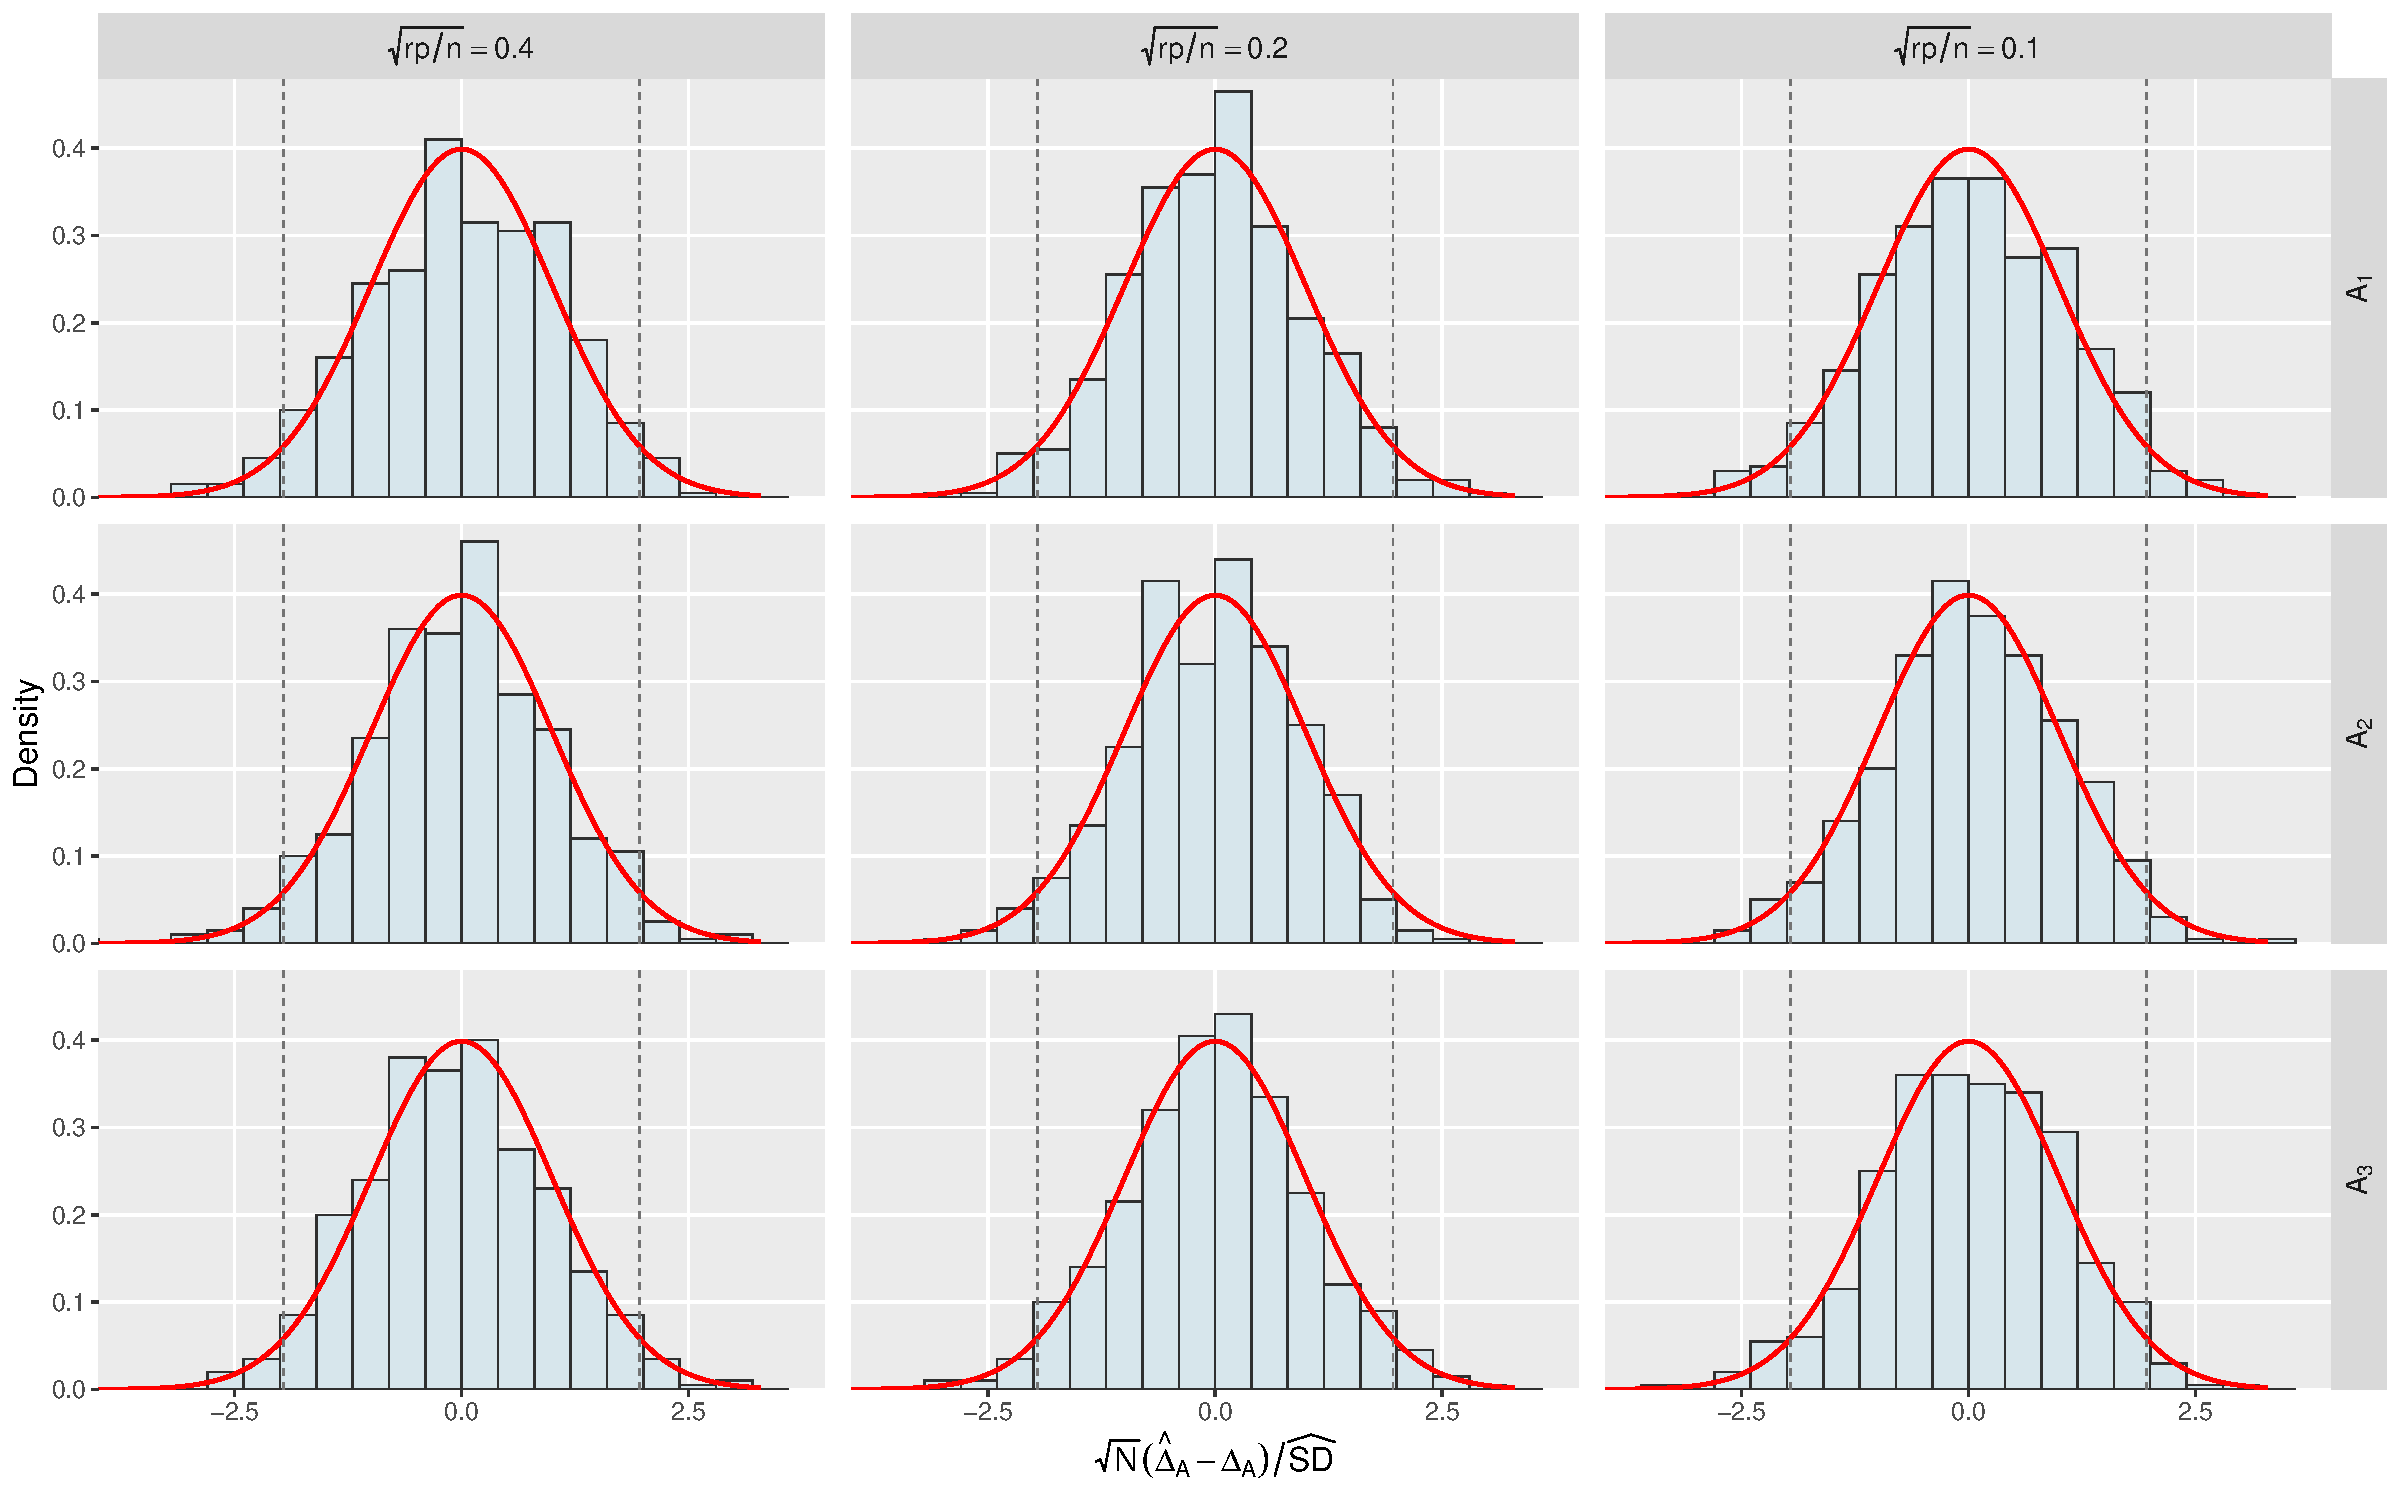
\includegraphics[width=0.7\textwidth]{figures/density_compare_sd1_inf_ind.pdf}
	\caption{Empirical densities of the studentized statistic $\sqrt{N}\,\widehat V^{-1/2}(\widehat\Delta_{\bA}-\Delta_{\bA})$ in matrix trace regression under identity covariance.}
	\label{fig:density-ind}
\end{figure}

\begin{figure}[!t]
	\centering
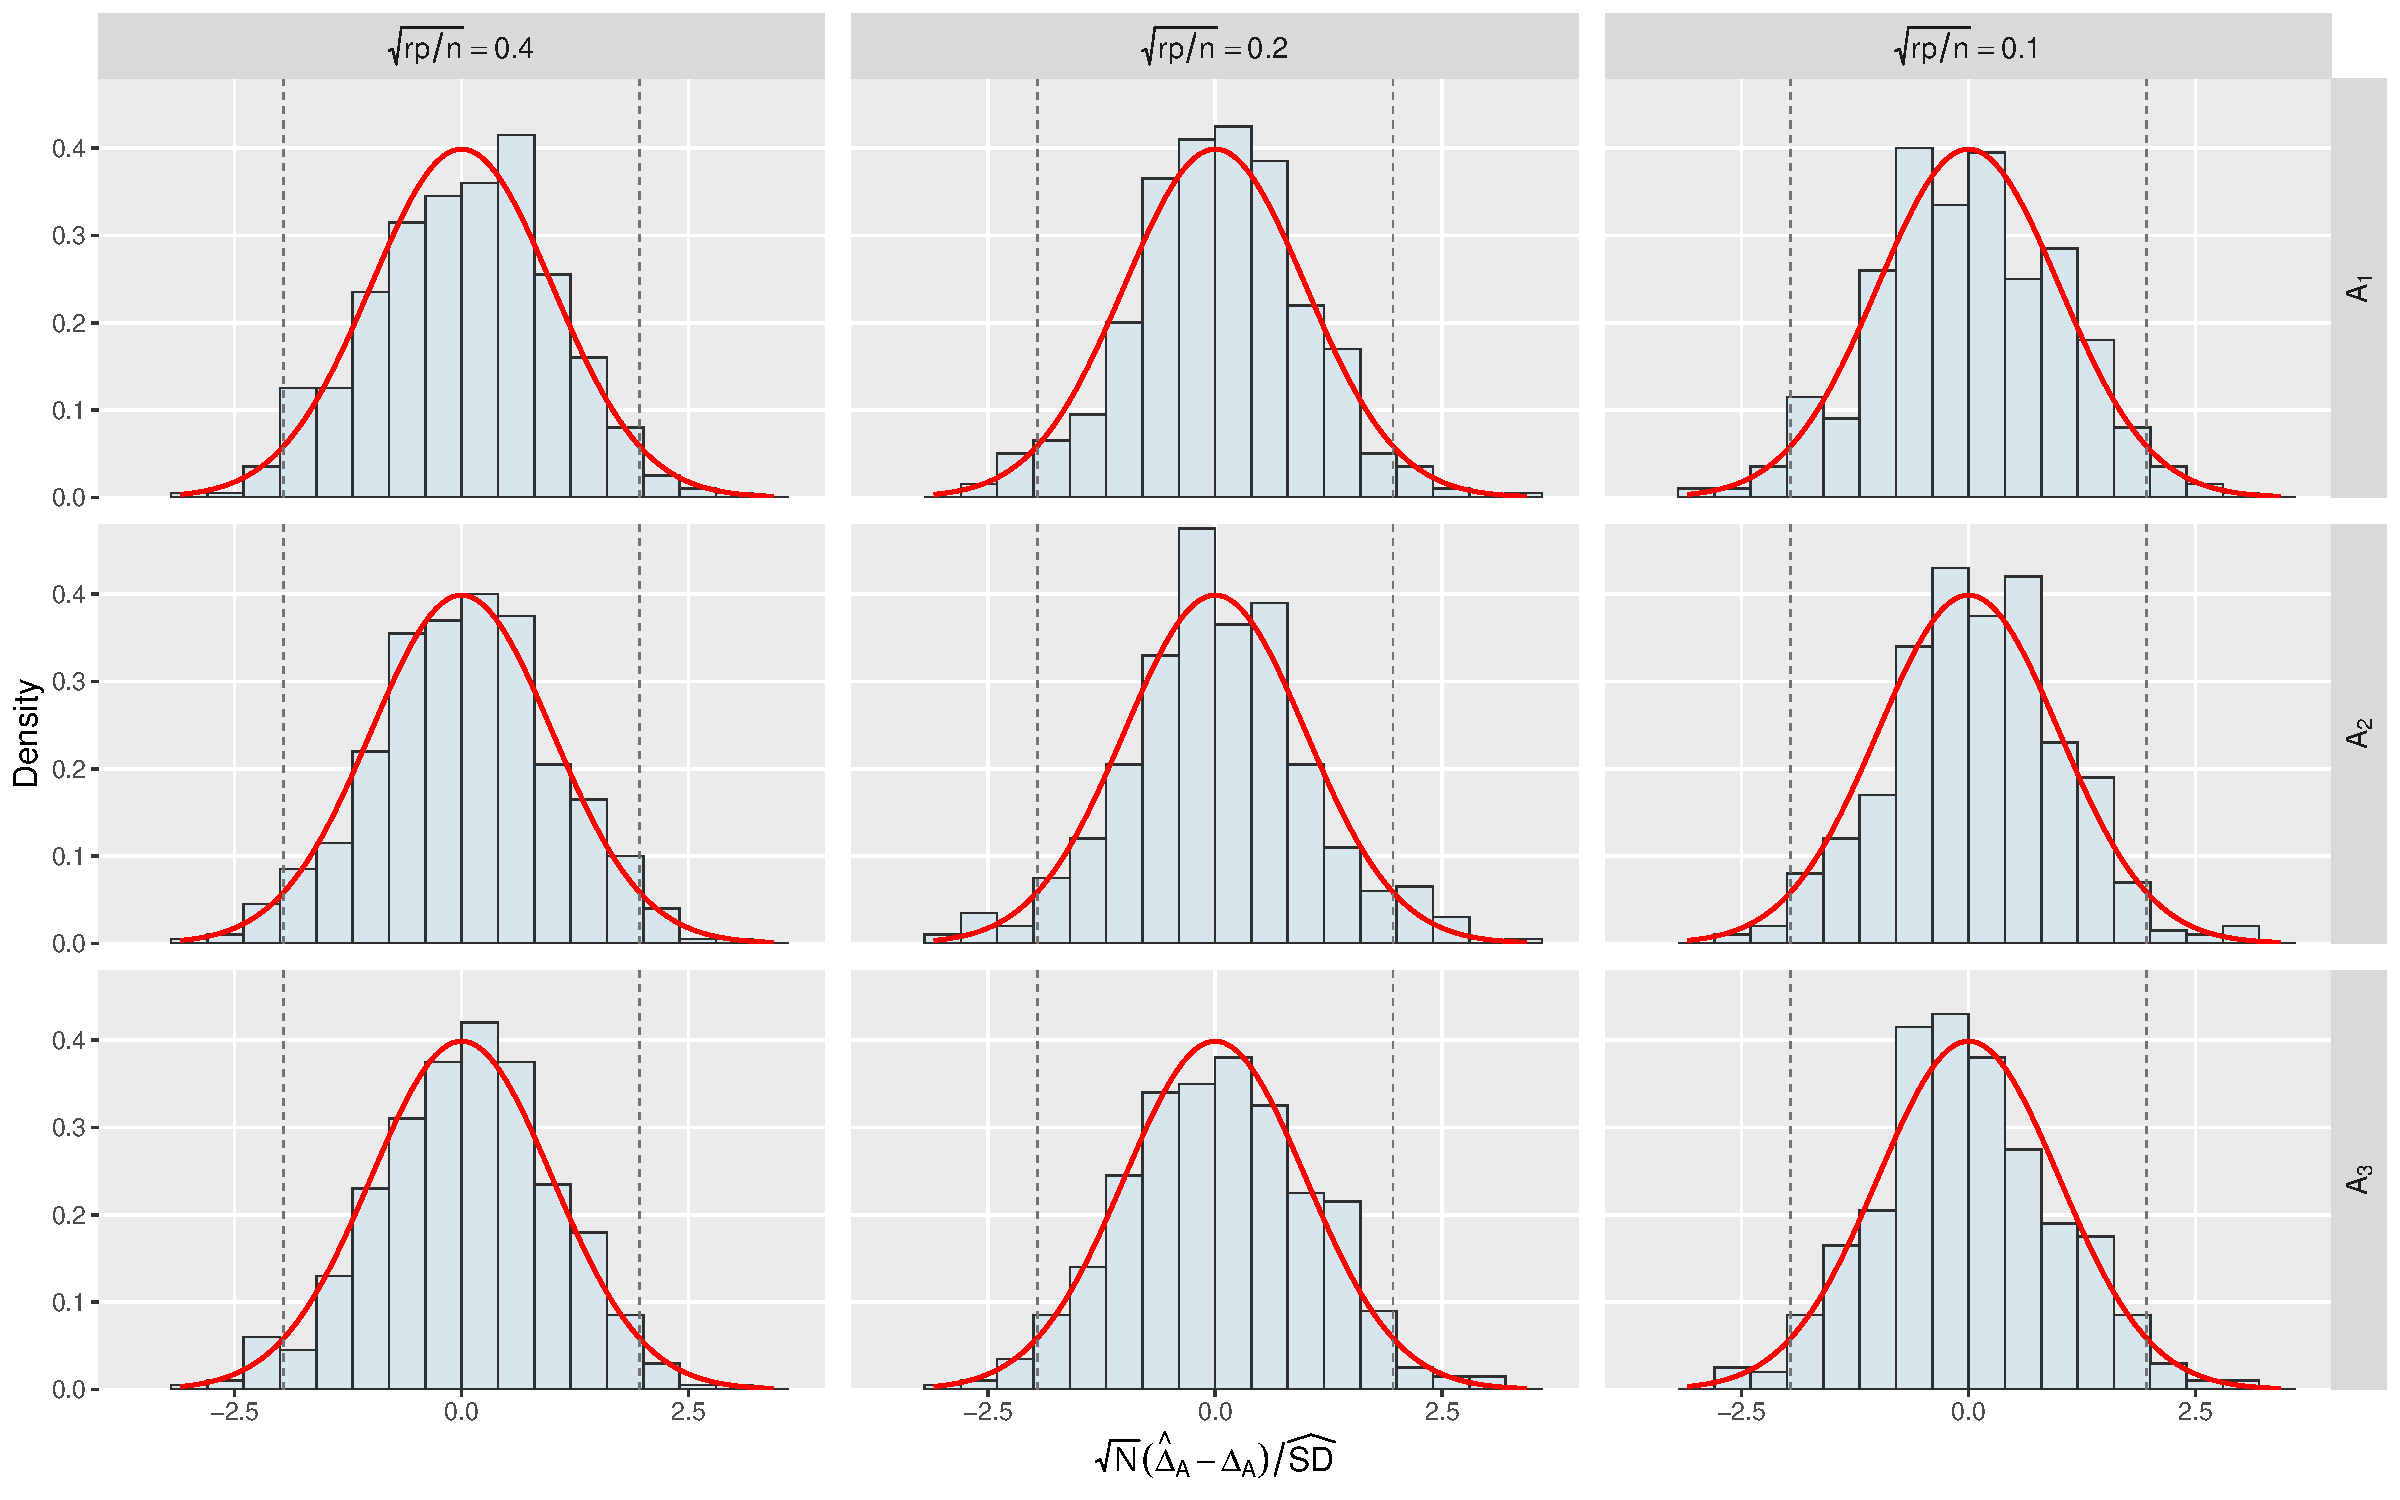
\includegraphics[width=0.7\textwidth]{figures/density_compare_all_settings_inf.pdf}
	\caption{Empirical densities of the studentized statistic $\sqrt{N}\,\widehat V^{-1/2}(\widehat\Delta_{\bA}-\Delta_{\bA})$ in matrix trace regression under general Kronecker covariance.}
	\label{fig:density-general}
\end{figure}

\begin{table}[!htbp]
\centering
\caption{Empirical coverage probabilities and average lengths of nominal 95\% Wald confidence intervals in matrix trace regression.}
\label{tab:cp-ci-sd1-combined}
%\scriptsize
\begin{threeparttable}
\setlength{\tabcolsep}{6pt}
\renewcommand{\arraystretch}{1.05}
\begin{tabular}{cc|cc|cc}
\toprule
\multirow{2}{*}{$A$} & \multirow{2}{*}{$\sqrt{rp/n}$} & \multicolumn{2}{c|}{Identity covariance} & \multicolumn{2}{c}{General Kronecker covariance} \\
\cmidrule(lr){3-4}\cmidrule(l){5-6}
 &  & CP & Avg. length & CP & Avg. length \\
\midrule
\multirow{3}{*}{1}
 & 0.4  & 0.948 & 0.0596 & 0.956 & 0.0653 \\
 & 0.2  & 0.956 & 0.0295 & 0.948 & 0.0320 \\
 & 0.1  & 0.944 & 0.0147 & 0.950 & 0.0159 \\
\midrule
\multirow{3}{*}{2}
 & 0.4  & 0.950 & 0.0572 & 0.948 & 0.0593 \\
 & 0.2  & 0.960 & 0.0283 & 0.932 & 0.0293 \\
 & 0.1  & 0.952 & 0.0141 & 0.966 & 0.0146 \\
\midrule
\multirow{3}{*}{3}
 & 0.4  & 0.950 & 0.0530 & 0.946 & 0.0558 \\
 & 0.2  & 0.944 & 0.0262 & 0.950 & 0.0276 \\
 & 0.1  & 0.944 & 0.0131 & 0.958 & 0.0138 \\
\bottomrule
\end{tabular}
\end{threeparttable}
\end{table}


Tables~\ref{tab:five-methods-ind} and \ref{tab:five-methods-general} report bias and RMSE.
Two features are consistent across designs.
First, exploiting the low-rank matrix structure is essential: all structured competitors dominate Vec-DB.
Second, the benefit of covariance weighting is most visible under dependence.
Under identity covariance, OS-DB is comparable to TS-DB and the two power-iteration refinements, with PI-nosplit occasionally yielding a slightly smaller RMSE.
Under general Kronecker covariance, OS-DB is typically first or second in RMSE across loadings and remains uniformly stable, whereas the vectorized procedure deteriorates markedly.

The inferential results are aligned with the asymptotic theory.
Figures~\ref{fig:density-ind} and \ref{fig:density-general} show that the studentized statistic $\sqrt{N}\,\widehat V^{-1/2}(\widehat\Delta_{\bA}-\Delta_{\bA})$ is already close to Gaussian in moderate samples, with the approximation improving as $\sqrt{rp/n}$ decreases.
Table~\ref{tab:cp-ci-sd1-combined} shows empirical coverage near the nominal $95\%$ level and interval length decreasing monotonically with the sample size.
Intervals under general Kronecker covariance are modestly longer, reflecting the additional error from estimating the covariance structure.
Thus, in the matrix model, OS-DB delivers accurate Wald inference without sacrificing estimation efficiency.

\subsection{Tucker tensor regression}
For three-way Tucker tensor regression, we generate covariates by
\[
\mathcal X_i=\mathcal S_i\times_1 \bL_1\times_2 \bL_2\times_3 \bL_3,
\qquad i=1,\ldots,N,
\]
where $N=2n$ and the entries of $\mathcal S_i\in\mathbb R^{p\times p\times p}$ are i.i.d.\ standard normal.
We set $p_1=p_2=p_3=p=30$, $r_1=r_2=r_3=r=2$, and $\sigma=1$.
The true tensor coefficient is
\[
\mathcal T^\ast=\mathcal G^\ast\times_1\bU_1^\ast\times_2\bU_2^\ast\times_3\bU_3^\ast,
\]
where $\bU_1^\ast,\bU_2^\ast,\bU_3^\ast\in\mathbb R^{p\times r}$ are orthonormalized Gaussian matrices and the core tensor $\mathcal G^\ast\in\mathbb R^{r\times r\times r}$ has two nonzero entries, equal to one at $(1,1,1)$ and $(2,2,2)$.
The response is generated from
\[
y_i=\langle \mathcal X_i,\mathcal T^\ast\rangle+\varepsilon_i,
\qquad
\varepsilon_i\stackrel{\mathrm{iid}}{\sim}N(0,\sigma^2).
\]

As in the matrix case, we study two covariance settings.
Under identity covariance, $\bL_1=\bL_2=\bL_3=\bI_p$.
Under general Kronecker covariance, we set $\bL_j=\bQ_j\bLambda^{1/2}$ for $j=1,2,3$, where $\bQ_j$ are random orthogonal matrices and
\[
\bLambda=\mathrm{diag}\Big(\underbrace{2,\ldots,2}_{\lfloor p/4\rfloor},
\underbrace{1,\ldots,1}_{p-2\lfloor p/4\rfloor},
\underbrace{0.5,\ldots,0.5}_{\lfloor p/4\rfloor}\Big).
\]
Then each mode covariance matrix $\bSigma_{p_j}=\bL_j\bL_j^\top$ is unknown and is estimated by \eqref{eq:cov3}--\eqref{eq:cov4}, together with the induced Kronecker covariance \eqref{eq:deign_tensor}.

For the target functional $\Delta_{\mA}=\langle \mA,\mT^\ast\rangle$, we consider three loading tensors:
\begin{enumerate}[label=(\roman*)]
	\item $\mA_1$ has a single nonzero entry equal to one at $(1,1,1)$;
	\item $\mA_2=\bba^{\otimes 3}/\|\bba^{\otimes 3}\|_F$, where $\bba\in\mathbb R^p$ has its first $2\lfloor p^{1/4}\rfloor$ entries equal to one and the remaining entries zero;
	\item $\mA_3$ has i.i.d.\ standard normal entries and is normalized to Frobenius norm one.
\end{enumerate}
These again represent sparse, structured, and dense directions.

We compare OS-DB with two iterative projection refinements, IT-split and IT-nosplit, together with the vectorized baseline Vec-DB.
Each configuration is repeated 500 times, with
\[
\sqrt{rp/n}\in\{0.4,0.2,0.1\}.
\]

\begin{table}[!htbp]
\centering
\caption{Finite-sample bias and RMSE of four debiasing methods for Tucker tensor regression under identity covariance. The best and second-best values are shown in \textbf{bold} and \underline{underlined}, respectively.}
\label{tab:tsr-methods-ind}
%\scriptsize
\begin{threeparttable}
\setlength{\tabcolsep}{4pt}
\begin{tabular}{lllcccc}
\toprule
$A$ & $\sqrt{rp/n}$ & Metric & OS-DB & IT-split & IT-nosplit & Vec-DB \\
\midrule
1 & 0.4 & Bias ($\times 10^{-3}$) & 4.954 & \underline{4.911} & \textbf{1.190} & -94.833 \\
 &  & RMSE & \textbf{0.0743} & \underline{0.0780} & 0.0851 & 1.0608 \\
1 & 0.2 & Bias ($\times 10^{-3}$) & \textbf{-1.841} & -3.378 & \underline{-2.160} & -35.766 \\
 &  & RMSE & \textbf{0.0757} & \underline{0.0767} & 0.0770 & 0.9729 \\
1 & 0.1 & Bias ($\times 10^{-3}$) & \underline{-0.316} & \textbf{-0.209} & 0.345 & -4.411 \\
 &  & RMSE & \textbf{0.0769} & \underline{0.0771} & 0.0773 & 1.0216 \\
\midrule
2 & 0.4 & Bias ($\times 10^{-3}$) & \textbf{-0.660} & -6.619 & \underline{1.076} & -19.485 \\
 &  & RMSE & \textbf{0.0926} & \underline{0.0952} & 0.1028 & 1.1380 \\
2 & 0.2 & Bias ($\times 10^{-3}$) & \underline{3.562} & \textbf{3.049} & 4.583 & -10.784 \\
 &  & RMSE & \underline{0.1005} & 0.1015 & \textbf{0.1000} & 0.9794 \\
2 & 0.1 & Bias ($\times 10^{-3}$) & \textbf{2.533} & \underline{2.614} & 3.045 & -15.737 \\
 &  & RMSE & \underline{0.0958} & 0.0965 & \textbf{0.0956} & 0.9808 \\
\midrule
3 & 0.4 & Bias ($\times 10^{-3}$) & \textbf{-0.307} & 5.864 & \underline{-3.976} & 64.080 \\
 &  & RMSE & \textbf{0.0741} & \underline{0.0754} & 0.0821 & 1.1262 \\
3 & 0.2 & Bias ($\times 10^{-3}$) & \underline{2.184} & 3.149 & \textbf{2.048} & 4.573 \\
 &  & RMSE & \textbf{0.0701} & \underline{0.0710} & 0.0721 & 0.9999 \\
3 & 0.1 & Bias ($\times 10^{-3}$) & \underline{6.734} & 7.116 & \textbf{6.435} & 26.993 \\
 &  & RMSE & \underline{0.0720} & 0.0723 & \textbf{0.0716} & 0.9866 \\
\bottomrule
\end{tabular}
\end{threeparttable}
\end{table}

\begin{table}[!htbp]
\centering
\caption{Finite-sample bias and RMSE of four debiasing methods for Tucker tensor regression under general Kronecker covariance. The best and second-best values are shown in \textbf{bold} and \underline{underlined}, respectively.}
\label{tab:tsr-methods-general}
%\scriptsize
\begin{threeparttable}
\setlength{\tabcolsep}{4pt}
\begin{tabular}{lllcccc}
\toprule
$A$ & $\sqrt{rp/n}$ & Metric & OS-DB & IT-split & IT-nosplit & Vec-DB \\
\midrule
1 & 0.4 & Bias ($\times 10^{-3}$) & \textbf{1.663} & \underline{-6.176} & 27.673 & -10.754 \\
 &  & RMSE & \textbf{0.0482} & \underline{0.0675} & 0.0818 & 1.2638 \\
1 & 0.2 & Bias ($\times 10^{-3}$) & \underline{-1.833} & \textbf{-0.823} & 10.059 & -14.346 \\
 &  & RMSE & \textbf{0.0476} & \underline{0.0639} & 0.0643 & 1.1646 \\
1 & 0.1 & Bias ($\times 10^{-3}$) & \underline{-2.138} & -4.793 & \textbf{0.761} & -70.728 \\
 &  & RMSE & \textbf{0.0456} & 0.0603 & \underline{0.0598} & 1.1080 \\
\midrule
2 & 0.4 & Bias ($\times 10^{-3}$) & \textbf{-3.595} & -15.488 & -28.272 & \underline{-11.192} \\
 &  & RMSE & \textbf{0.0493} & \underline{0.0668} & 0.0697 & 1.4080 \\
2 & 0.2 & Bias ($\times 10^{-3}$) & \underline{-2.042} & -4.943 & -10.309 & \textbf{0.293} \\
 &  & RMSE & \textbf{0.0510} & 0.0659 & \underline{0.0647} & 1.1762 \\
2 & 0.1 & Bias ($\times 10^{-3}$) & \underline{-2.006} & -7.616 & -9.738 & \textbf{0.885} \\
 &  & RMSE & \textbf{0.0505} & 0.0632 & \underline{0.0624} & 1.0673 \\
\midrule
3 & 0.4 & Bias ($\times 10^{-3}$) & \textbf{-0.426} & \underline{-8.284} & -9.460 & -20.300 \\
 &  & RMSE & \textbf{0.0943} & \underline{0.1209} & 0.1401 & 1.4010 \\
3 & 0.2 & Bias ($\times 10^{-3}$) & \underline{-4.188} & \textbf{-2.134} & -8.554 & 46.489 \\
 &  & RMSE & \textbf{0.0905} & 0.1175 & \underline{0.1162} & 1.1230 \\
3 & 0.1 & Bias ($\times 10^{-3}$) & \textbf{0.878} & \underline{1.965} & -2.452 & -31.359 \\
 &  & RMSE & \textbf{0.0918} & 0.1123 & \underline{0.1111} & 1.1348 \\
\bottomrule
\end{tabular} 
\end{threeparttable}
\end{table}


\begin{figure}[!t]
	\centering
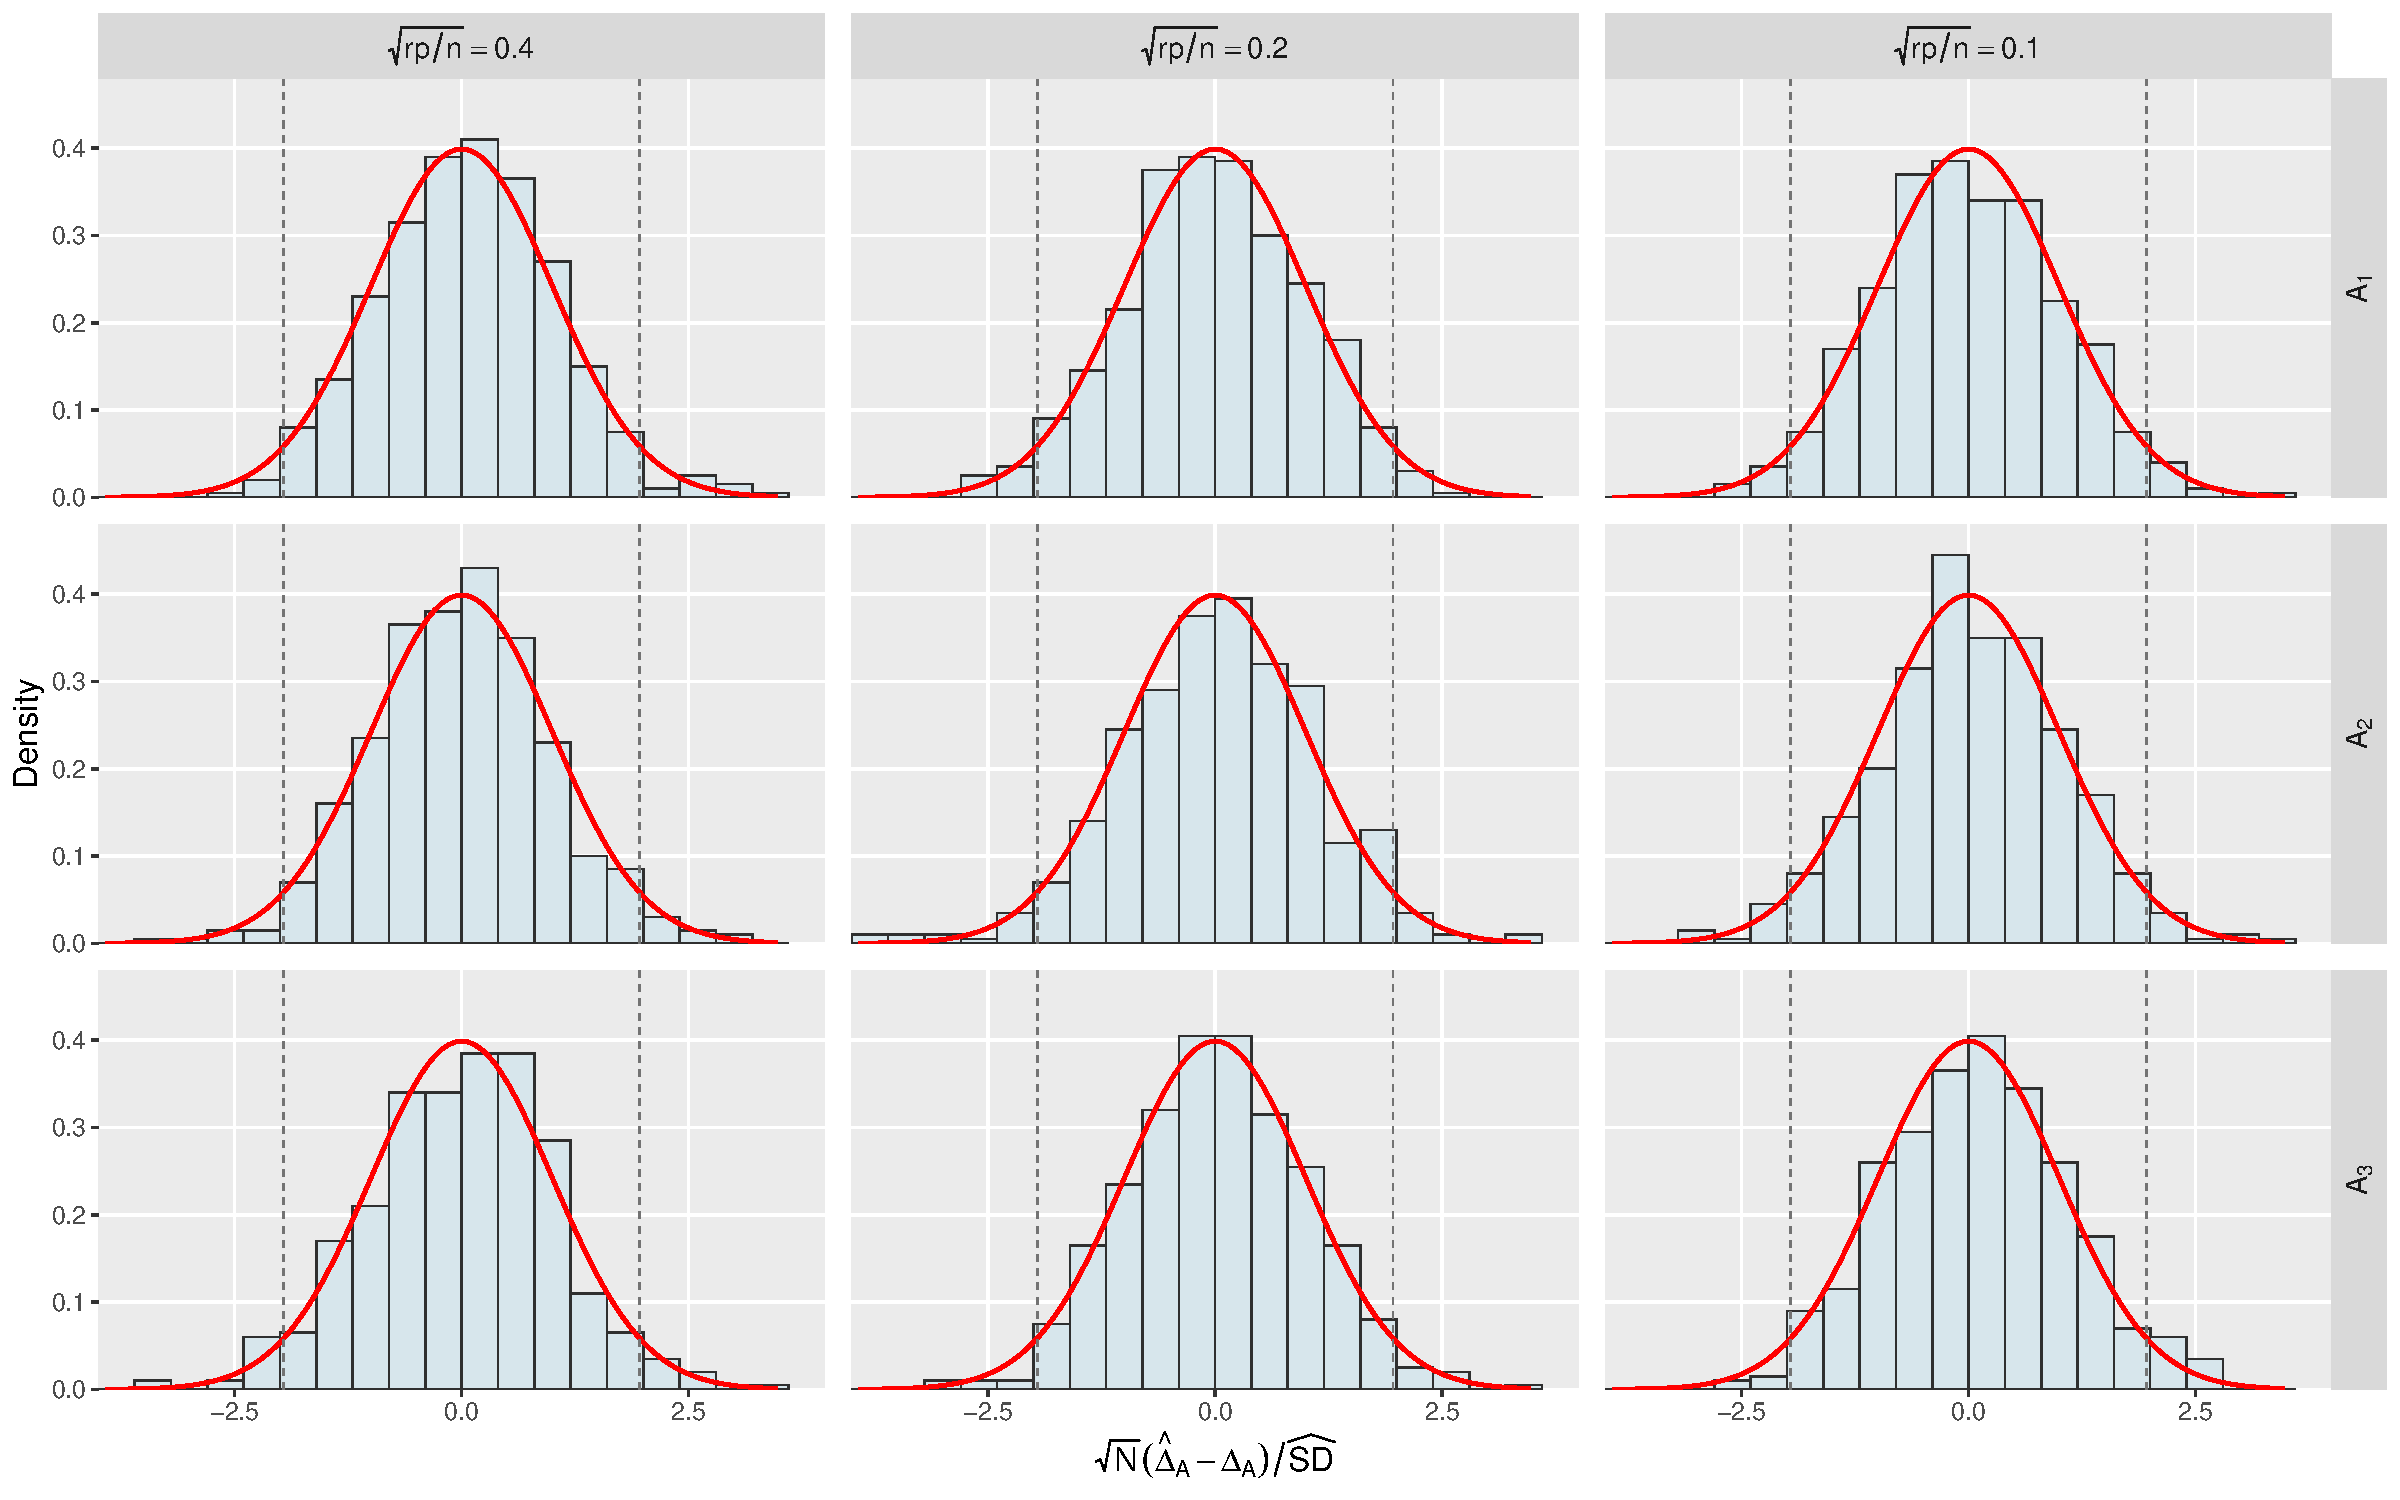
\includegraphics[width=0.7\textwidth]{figures/density_tsr_compare_sd1_inf_ind.pdf}
	\caption{Empirical densities of the studentized statistic $\sqrt{N}\,\widehat V^{-1/2}(\widehat\Delta_{\mA}-\Delta_{\mA})$ in Tucker tensor regression under identity covariance.}
	\label{fig:tsr-density-ind}
\end{figure}

\begin{figure}[!t]
	\centering
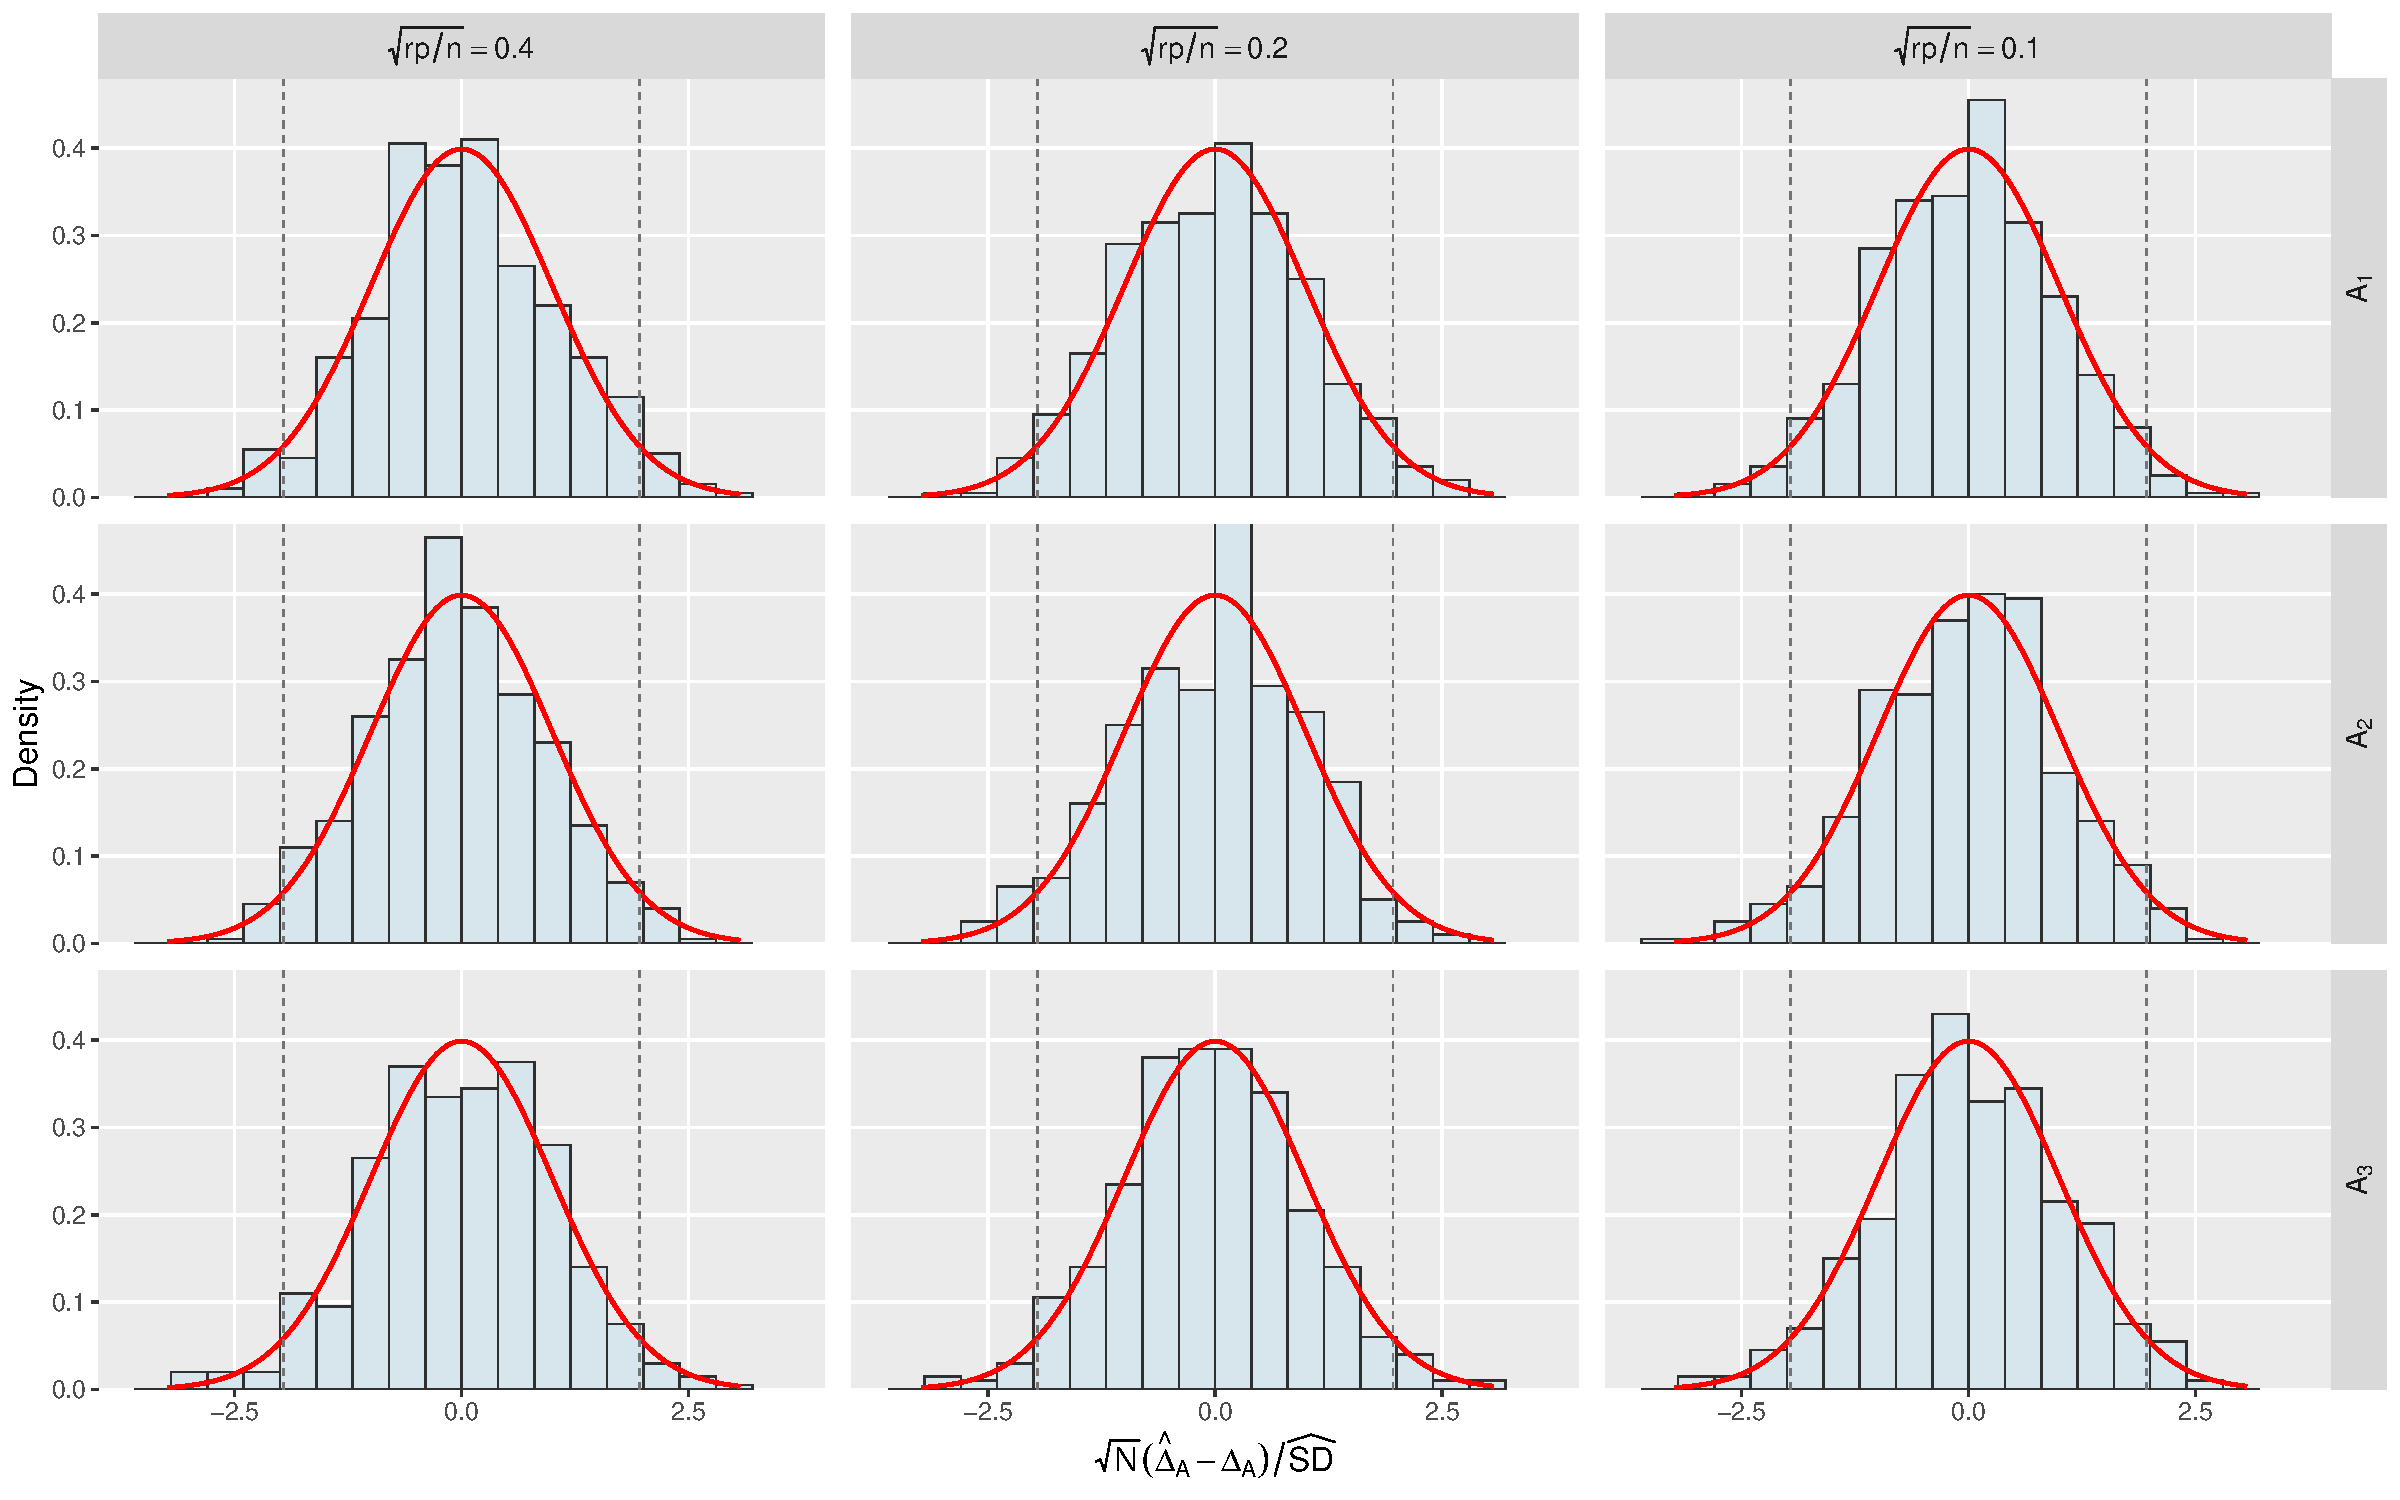
\includegraphics[width=0.7\textwidth]{figures/density_tsr_compare_sd1_inf.pdf}
	\caption{Empirical densities of the studentized statistic $\sqrt{N}\,\widehat V^{-1/2}(\widehat\Delta_{\mA}-\Delta_{\mA})$ in Tucker tensor regression under general Kronecker covariance.}
	\label{fig:tsr-density}
\end{figure}

\begin{table}[!htbp]
\centering
\caption{Empirical coverage probabilities and average lengths of nominal 95\% Wald confidence intervals in Tucker tensor regression.}
\label{tab:tsr-cp-ci-sd1-combined}
%\scriptsize
\begin{threeparttable}
\setlength{\tabcolsep}{6pt}
\renewcommand{\arraystretch}{1.05}
\begin{tabular}{cc|cc|cc}
\toprule
\multirow{2}{*}{$A$} & \multirow{2}{*}{$\sqrt{rp/n}$} & \multicolumn{2}{c|}{Identity covariance} & \multicolumn{2}{c}{General Kronecker covariance} \\
\cmidrule(lr){3-4}\cmidrule(l){5-6}
 &  & CP & Avg. length & CP & Avg. length \\
\midrule
\multirow{3}{*}{1}
 & 0.4  & 0.960 & 0.0110 & 0.940 & 0.0068 \\
 & 0.2  & 0.958 & 0.0055 & 0.948 & 0.0034 \\
 & 0.1  & 0.954 & 0.0027 & 0.958 & 0.0017 \\
\midrule
\multirow{3}{*}{2}
 & 0.4  & 0.960 & 0.0137 & 0.962 & 0.0074 \\
 & 0.2  & 0.948 & 0.0068 & 0.944 & 0.0036 \\
 & 0.1  & 0.950 & 0.0034 & 0.942 & 0.0018 \\
\midrule
\multirow{3}{*}{3}
 & 0.4  & 0.938 & 0.0104 & 0.946 & 0.0133 \\
 & 0.2  & 0.966 & 0.0052 & 0.954 & 0.0065 \\
 & 0.1  & 0.946 & 0.0026 & 0.942 & 0.0033 \\
\bottomrule
\end{tabular}
\end{threeparttable}
\end{table}


Tables~\ref{tab:tsr-methods-ind} and \ref{tab:tsr-methods-general} summarize bias and RMSE.
The same pattern reappears in the Tucker model.
Methods that exploit low Tucker rank uniformly improve on Vec-DB, and the improvement is largest under correlated designs.
Under identity covariance, OS-DB is typically among the best procedures and is close to IT-nosplit in RMSE.
Under general Kronecker covariance, OS-DB attains the smallest RMSE in all reported settings while keeping the bias uniformly small.

The inferential conclusions are again consistent with the theory.
Figures~\ref{fig:tsr-density-ind} and \ref{fig:tsr-density} show that the studentized statistic is close to Gaussian, apart from mild finite-sample skewness in the smallest-sample regime.
Table~\ref{tab:tsr-cp-ci-sd1-combined} shows empirical coverage near $95\%$ and interval length decreasing with the sample size.
Dense directions are more difficult, especially under correlated designs, and consequently yield longer intervals.
Overall, the tensor experiments indicate that OS-DB retains the expected inferential calibration while remaining competitive in point estimation.

\section{Real data analysis}\label{sec:realdata}
We illustrate the proposed inference procedures using resting-state EEG data from the Healthy Brain Network \citep{Alexander2017HBN}. The response variable is age, and the covariates are region-by-frequency summaries derived from eyes-closed (EC) and eyes-open (EO) resting-state recordings. The purpose of this analysis is not merely to assess predictive performance, but to show how the proposed method enables valid inference for scientifically interpretable linear functionals of a low-rank coefficient matrix or tensor.

The raw data are drawn from HBN releases R1--R4. After merging the release-level participant files, we obtain 794 unique participant entries, among which 792 have a resting-state EEG file. We retain subjects with a matched age measurement and usable data in both EC and EO conditions after preprocessing and quality control. The final sample contains 397 subjects, with ages ranging from 5.04 to 21.00 years.

EEG recordings are acquired from the 129-channel EGI montage. After standard filtering, artifact annotation, bad-channel detection, interpolation, rereferencing, and epoch screening, we compute band power from clean epochs using Welch's method. Power is integrated over eight canonical frequency bands: delta, theta, alpha1, alpha2, beta1, beta2, gamma1, and gamma2. Channel-level power is then averaged within ten prespecified ROI groups, yielding either a $10\times 8$ matrix covariate for a single condition or a $10\times 8\times 2$ tensor covariate after stacking EC and EO along the condition mode. The exact ROI grouping is reported in Table~\ref{tab:realdata-roi}.

Throughout this section, all tuning parameters are selected by cross-validation, and all loadings used for inference are normalized to have Frobenius norm one. The inferential targets are fixed \emph{a priori}. Specifically, we consider ROI-slice loadings, band-slice loadings, and global loadings in the matrix model; and, in the tensor model, we additionally consider shared and contrast loadings along the EC/EO mode. These targets correspond to interpretable summaries of the coefficient object and are therefore natural candidates for uncertainty quantification.

\begin{table}[!t]
\centering
\scriptsize
\caption{Coordinate-based aggregation from the 129-channel EGI montage to the 10 ROI groups. ROI-level band power is obtained by averaging the channel-level band power within each group.}
\label{tab:realdata-roi}
\renewcommand{\arraystretch}{1.05}
\begin{tabular}{@{}lcp{0.75\textwidth}@{}}
\toprule
ROI group & $n$ & Channels \\
\midrule
anterior-midline & 12 & Cz, E5, E6, E7, E11, E12, E14, E15, E16, E17, E21, E106 \\
frontal-left & 13 & E13, E18, E19, E20, E22, E23, E24, E25, E26, E27, E28, E32, E33 \\
frontal-right & 13 & E1, E2, E3, E4, E8, E9, E10, E112, E117, E118, E122, E123, E124 \\
central-left & 13 & E29, E30, E31, E34, E35, E36, E37, E39, E40, E41, E42, E45, E46 \\
central-right & 13 & E80, E87, E93, E102, E103, E104, E105, E108, E109, E110, E111, E115, E116 \\
temporal-left & 10 & E38, E43, E44, E48, E49, E56, E63, E68, E127, E128 \\
temporal-right & 10 & E94, E99, E107, E113, E114, E119, E120, E121, E125, E126 \\
posterior-left & 18 & E47, E50, E51, E52, E53, E54, E57, E58, E59, E60, E61, E64, E65, E66, E67, E69, E70, E73 \\
posterior-midline & 9 & E55, E62, E71, E72, E74, E75, E76, E81, E82 \\
posterior-right & 18 & E77, E78, E79, E83, E84, E85, E86, E88, E89, E90, E91, E92, E95, E96, E97, E98, E100, E101 \\
\bottomrule
\end{tabular}
\end{table}


\subsection{Matrix regression analysis}
We consider a low-rank matrix regression model using the log-contrast covariate
\[
\log_{10}(\mathrm{EC})-\log_{10}(\mathrm{EO}).
\]
Five-fold cross-validation selects rank 1 for this model, and we base the matrix inference on the resulting rank-1 fit.

For this model, each loading admits a straightforward interpretation. An ROI-slice loading represents the average age association of the EC--EO contrast within one anatomical region after averaging over all frequency bands. A band-slice loading represents the analogous age association for one frequency band after averaging over ROIs. A global loading averages over the full $10\times 8$ matrix and tests whether the overall association is diffuse across entries.

Figure~\ref{fig:realdata-matrix} reports point estimates and nominal 95\% confidence intervals for these prespecified loadings. The evidence is sparse rather than diffuse. At the ROI level, the anterior-midline loading is significantly positive, whereas the central-right loading is significantly negative. At the band level, only the alpha2 loading remains significantly positive after averaging over ROIs. The global loading is not significantly different from zero. At the more local single-entry level, six loadings have confidence intervals excluding zero, and these are concentrated in the theta and alpha2 bands within the anterior-midline, frontal-left, and central-right regions. Hence the fitted rank-1 log-contrast matrix does not suggest a matrix-wide age effect; instead, it points to a small number of localized spatial-spectral summaries that are distinguishable from zero.

\begin{figure}[!t]
	\centering
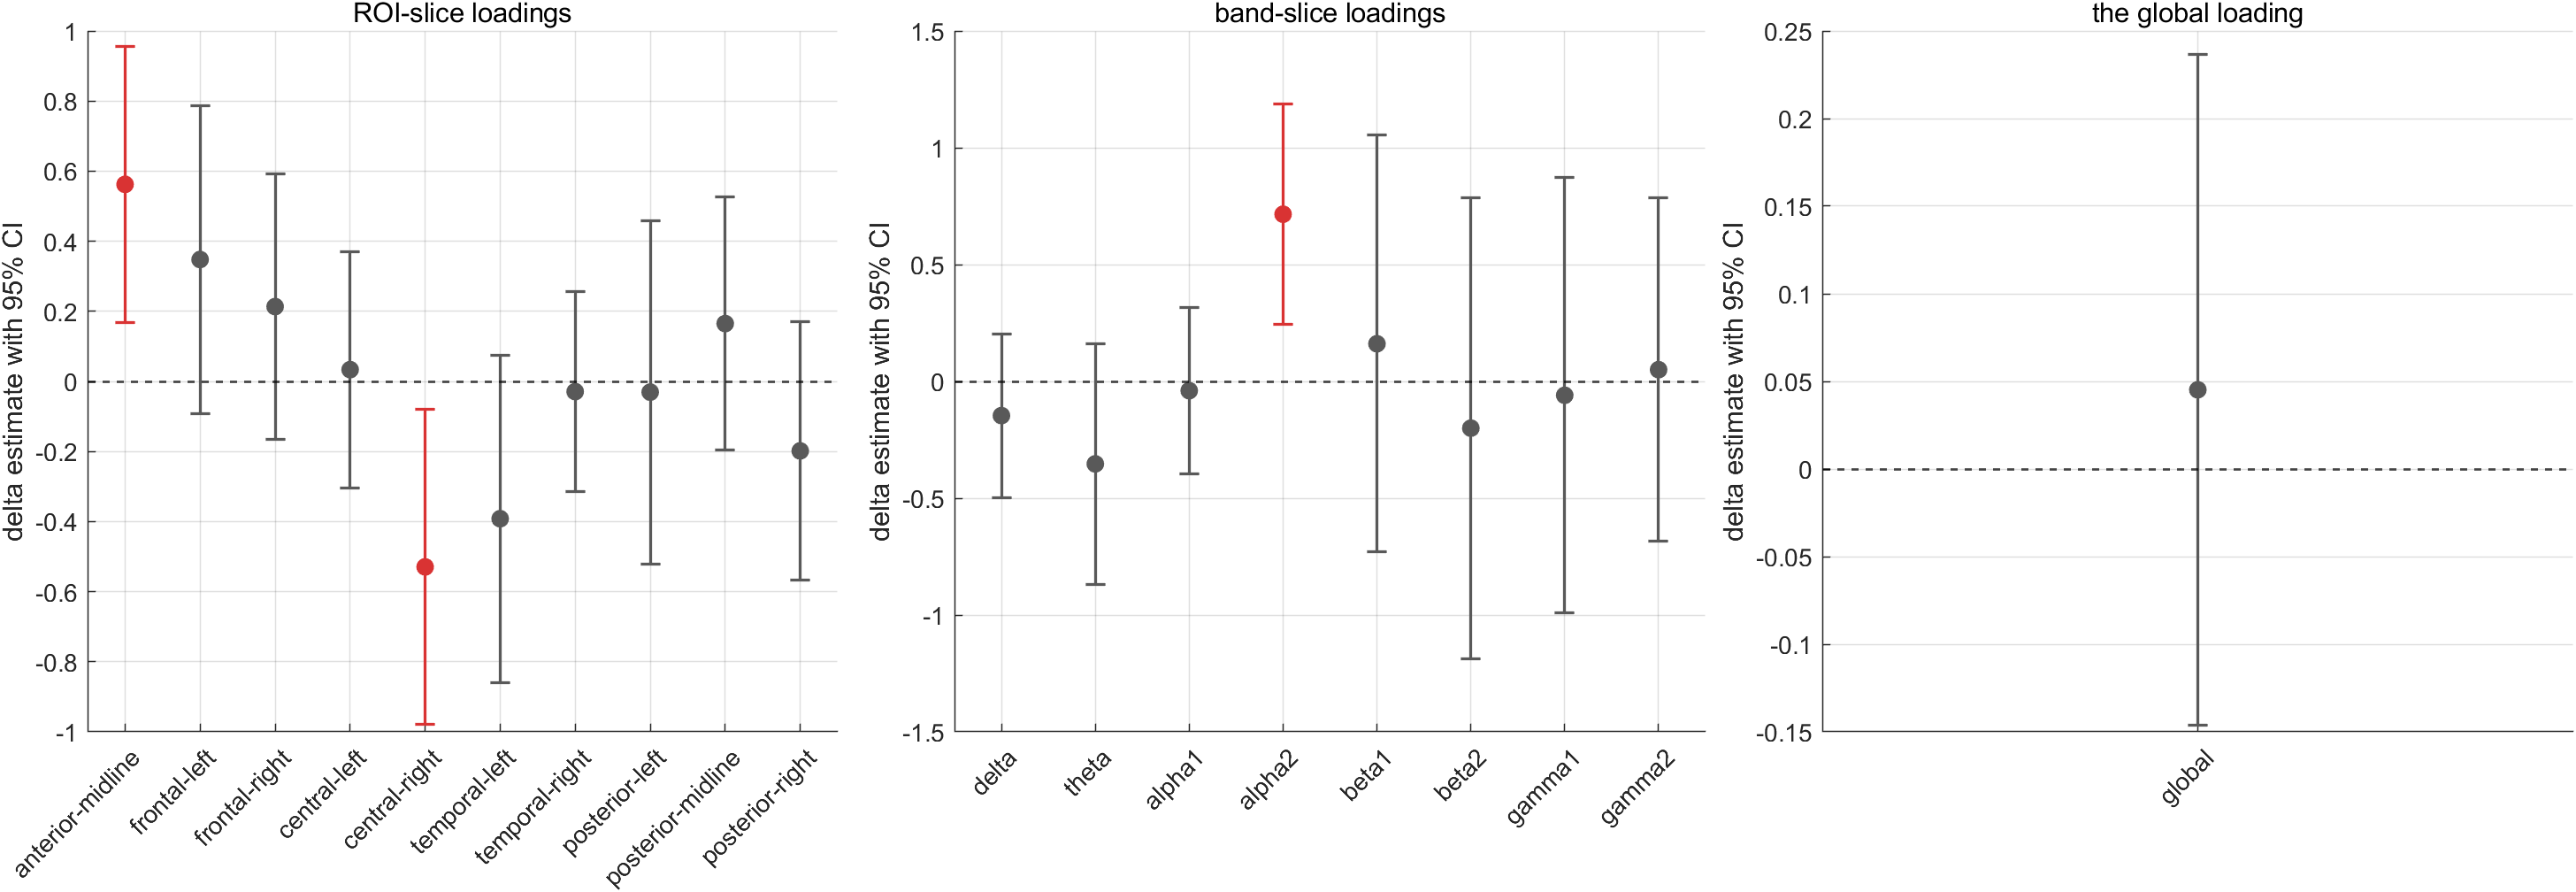
\includegraphics[width=0.98\textwidth]{figures/realdata_matrix_structured_loadings.png}
	\caption{Projection-based inference for prespecified loadings in the rank-1 matrix model with covariate $\log_{10}(\mathrm{EC})-\log_{10}(\mathrm{EO})$. Shown are point estimates and nominal 95\% confidence intervals for ROI-slice loadings, band-slice loadings, and the global loading. The fitted log-contrast model supports a sparse set of structured summaries, with significant evidence concentrated in anterior-midline, central-right, and alpha2 directions, while the global loading is not significantly different from zero.}
	\label{fig:realdata-matrix}
\end{figure}

Selected confidence intervals are reported in Panel A of Table~\ref{tab:realdata-infer}. This finding illustrates the inferential value of the proposed method. A low-rank point estimate alone may indicate that the log-contrast matrix is predictive of age, but it does not reveal whether the signal is globally diffuse or driven by localized effects. The projection-based intervals provide this additional resolution by identifying which prespecified summaries are statistically distinguishable from zero.

\subsection{Tensor regression analysis}
We next stack the log-transformed EC and EO matrices to form a $10\times 8\times 2$ tensor covariate and fit a Tucker tensor regression model with rank $(2,5,2)$,  which is also selected by CV.

The tensor formulation allows us to define scientifically meaningful loadings along the condition mode. In particular, the loading $(1,1)/\sqrt{2}$ targets the component shared by EC and EO, whereas $(1,-1)/\sqrt{2}$ targets the EC--EO contrast. Combining these condition-mode loadings with global, band-specific, or ROI-group loadings yields a family of interpretable functionals for inference. For the ROI-group analysis, the ten original ROIs are aggregated into three broader groups: anterior, central, and posterior.

Figure~\ref{fig:realdata-tensor} summarizes the resulting confidence intervals. Relative to the matrix log-contrast analysis, the tensor model shifts the evidence away from global summaries and toward frequency-specific shared and contrast structure. Neither the full-tensor loading, nor the condition-slice loadings, nor the shared-global or contrast-global summaries is significantly different from zero. At the ROI level, only the central-left slice remains significant. In contrast, the band-level evidence is much stronger: for the shared component, theta and gamma1 are significantly negative, whereas alpha2, beta1, and gamma2 are significantly positive; for the contrast component, theta, beta2, and gamma1 are significantly negative, whereas alpha1, beta1, and gamma2 are significantly positive. Among the broader ROI-group summaries, only the posterior shared loading is significantly positive. Thus the stacked EC/EO tensor does not support a diffuse common effect or a diffuse state-differential effect; instead, it indicates that the stable signal is concentrated in prespecified frequency-band summaries.

\begin{figure}[!t]
	\centering
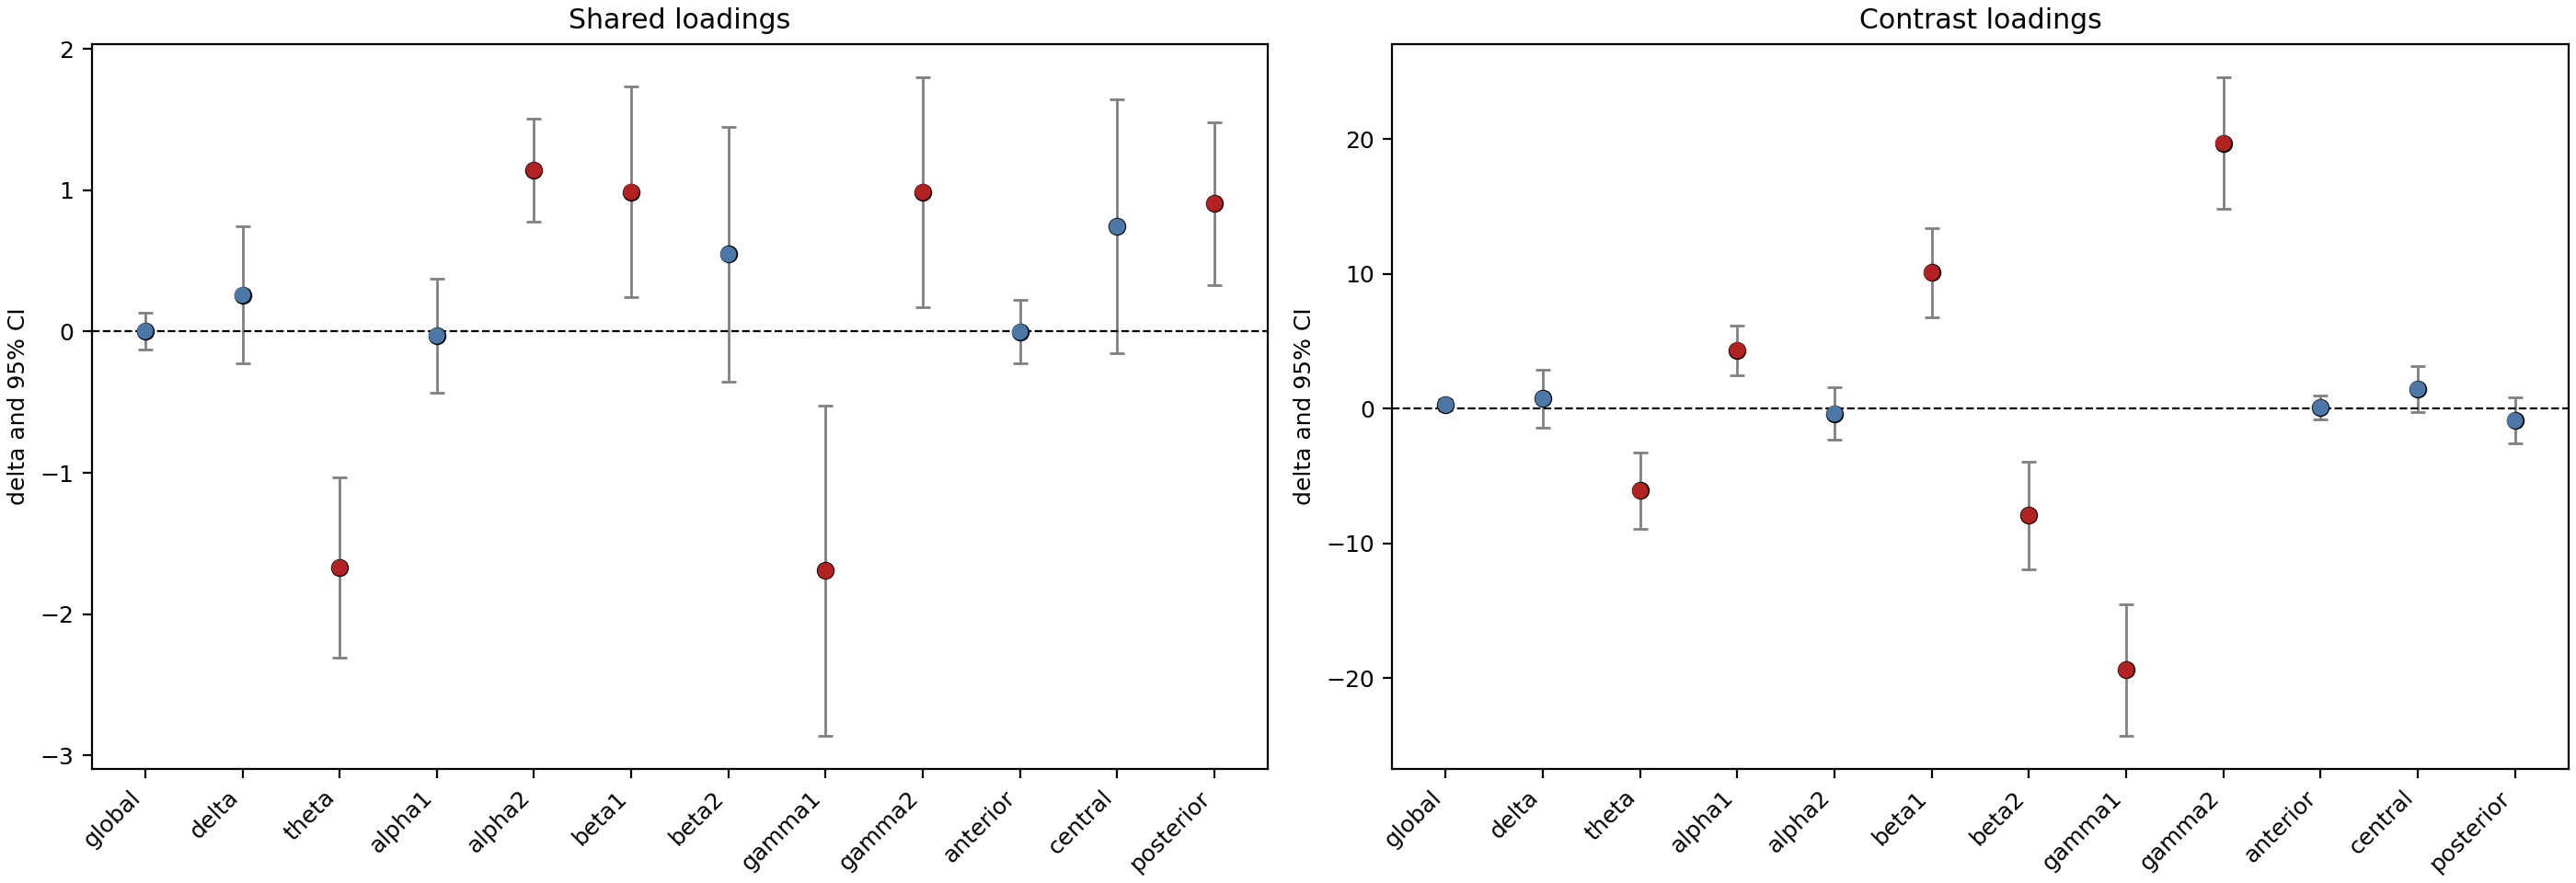
\includegraphics[width=0.98\textwidth]{figures/realdata_tensor_shared_contrast.png}
	\caption{Projection-based inference for prespecified shared and contrast loadings in the Tucker tensor model with fixed rank $(2,5,2)$. Point estimates and nominal 95\% confidence intervals are reported for global, band-specific, and ROI-group summaries. Under this fitted model, the stable evidence is concentrated in band-level shared and contrast summaries rather than in global or condition-level averages.}
	\label{fig:realdata-tensor}
\end{figure}

Selected intervals are reported in Panel B of Table~\ref{tab:realdata-infer}. The matrix and tensor analyses are not directly comparable entrywise because they are fit to different transformed covariates and parameterizations: the matrix model targets a single log-contrast matrix, whereas the tensor model decomposes stacked EC/EO effects into shared and contrast components. Their common message, however, is clear. In both analyses, the global summaries are not significant, so the age-related signal is not well described by a uniform shift over the entire coefficient object. The difference is interpretational: the matrix representation highlights a small number of localized ROI-band contrasts, whereas the tensor representation reveals broader band-specific shared and contrast patterns. This is precisely the type of conclusion enabled by the proposed projection-based inference framework.

\begin{table}[htbp]
	\centering
	\caption{Selected projection-based inference results for the HBN EEG analysis. Panel A reports point estimates and nominal 95\% confidence intervals for prespecified loadings under the rank-1 matrix model with covariate $\log_{10}(\mathrm{EC})-\log_{10}(\mathrm{EO})$. Panel B reports the corresponding results for prespecified shared and contrast loadings under the Tucker tensor model with fixed rank $(2,5,2)$. All loadings are normalized to have Frobenius norm one before inference. The reported intervals are pointwise and are not adjusted for multiplicity.}
	\label{tab:realdata-infer}
	\begin{threeparttable}
		\small
		\begin{tabular}{llcc}
			\toprule
			Loading & Description & Estimate & 95\% CI \\
			\midrule
			\multicolumn{4}{l}{\textbf{Panel A: Matrix log-contrast model, rank 1}} \\
			ROI slice & anterior-midline & $0.562$ & $[0.169,\,0.956]$ \\
			ROI slice & central-right & $-0.529$ & $[-0.979,\,-0.080]$ \\
			Band slice & alpha2 & $0.715$ & $[0.243,\,1.187]$ \\
			Global & all elements & $0.045$ & $[-0.146,\,0.237]$ \\
			\midrule
			\multicolumn{4}{l}{\textbf{Panel B: Tucker tensor model, fixed rank $(2,5,2)$}} \\
			Shared global & $(1,1)/\sqrt{2}$ over condition mode & $0.003$ & $[-0.126,\,0.133]$ \\
			Contrast global & $(1,-1)/\sqrt{2}$ over condition mode & $0.282$ & $[-0.110,\,0.673]$ \\
			ROI slice & central-left & $-0.611$ & $[-1.027,\,-0.194]$ \\
			Shared ROI group & posterior & $0.907$ & $[0.329,\,1.484]$ \\
			Shared band & theta & $-1.671$ & $[-2.307,\,-1.034]$ \\
			Shared band & alpha2 & $1.142$ & $[0.775,\,1.510]$ \\
			Shared band & gamma1 & $-1.692$ & $[-2.861,\,-0.524]$ \\
			Contrast band & alpha1 & $4.340$ & $[2.503,\,6.176]$ \\
			Contrast band & beta1 & $10.112$ & $[6.785,\,13.438]$ \\
			Contrast band & gamma1 & $-19.391$ & $[-24.283,\,-14.500]$ \\
			\bottomrule
		\end{tabular}
	\end{threeparttable}
\end{table}


\section{Conclusion}
This paper develops a unified projection-based inference framework for linear functionals in low-rank matrix and tensor regression under dependent designs. The central idea is to combine the local geometry of the low-rank parameter space with the covariance structure of the covariates through a covariance-weighted projection onto the tangent space. This projection yields an adjusted loading that serves as the appropriate inferential direction, and it leads naturally to a one-step debiased estimator for the target functional.

The proposed framework applies at an abstract level to low-rank manifold models and becomes fully implementable under Kronecker-type covariance structures. For low-rank matrix regression and Tucker tensor regression, we derive explicit forms of the projection operator, construct feasible estimators using covariance and subspace estimation, and justify sample-splitting / cross-fitting implementations. The resulting procedures support valid Wald-type confidence intervals and hypothesis tests for prespecified linear summaries of the coefficient object.

Our theoretical results show that both oracle and feasible estimators are asymptotically normal under suitable regularity conditions, and that the associated confidence intervals attain the local geometric benchmark determined by the projection direction. The simulation results further demonstrate that the proposed method achieves a favorable balance between inferential validity and efficiency, with especially strong performance under correlated designs where covariance-aware correction is essential. The EEG analysis illustrates the practical value of the framework: rather than producing only a low-rank point estimate, it enables direct uncertainty quantification for interpretable ROI-, band-, and condition-specific summaries.

More broadly, the paper highlights that valid inference in low-rank regression should account simultaneously for two sources of structure: the nonlinear geometry induced by the rank constraint and the dependence structure of the design. The covariance-weighted tangent-space projection developed here provides one principled way to achieve this goal. Possible future directions include extensions to generalized response models, adaptive rank uncertainty, alternative low-rank formats for third-order tensors, and inference under more general covariance structures beyond the Kronecker family.



\section{Appendix}

\subsection{Oracle estimate with independent initial estimate}

\begin{proof}[Proof of Theorem \ref{thm:asymp_normal}]
	According to \eqref{eq:err1}, 
	\[
	\widehat{\Delta}_A^{\mathrm{or}} - {\Delta}_A  = \frac{1}{N} \sum_{i=1}^N \langle {\Phi}(A), \mathcal{X}_i \rangle \varepsilon_i  + \Big\langle P_{{\Sigma},{\Theta}^\ast}^\ast(A) -   \frac{1}{N} \sum_{i=1}^N \langle  {\Phi}(A), \mathcal{X}_i \rangle     \mathcal{X}_i,  \widehat{\Theta} - \Theta^\ast\Big\rangle.
	\]  
	According to Assumptions \ref{cond:noise} and \ref{cond:design_general_vec},   $ \langle {\Phi}(A), \mathcal{X}_i \rangle \varepsilon_i$'s are i.i.d. with mean-zero. And $\| \langle {\Phi}(A), \mathcal{X}_i \rangle \varepsilon_i\|_{\psi_1}\leq \| \langle {\Phi}(A), \mathcal{X}_i \rangle\|_{\psi_2} \|\varepsilon_i\|_{\psi_2}\leq C \sigma \kappa\|{\Phi}(A)\|_{\Sigma}$. Then we have $\mbe| \langle {\Phi}(A), \mathcal{X}_i \rangle \varepsilon_i|^3 \leq C (\sigma \kappa\|{\Phi}(A)\|_{\Sigma} )^3$.
	Apply the Berry-Esseen Theorem 
	\be\label{eq4} \frac{1}{\sqrt{N}}V^{-1/2}  \sum_{i=1}^N \langle {\Phi}(A), \mathcal{X}_i \rangle \varepsilon_i \Rightarrow N(0, 1),\ee
	where $V  = \var(\langle {\Phi}(A), \mathcal{X}_i \rangle \varepsilon_i) = \sigma^2 \|  {\Phi}(A) \|_{\Sigma}^2$. 
	
	
	Note that $\wh\Theta$ is independent with the data samples and $ \langle  {\Phi}(A), \mathcal{X}_i \rangle\langle \mathcal{X}_i,  \widehat{\Theta} - \Theta^\ast\rangle $'s are i.i.d. and 
	$$\mbe\big[ \langle  {\Phi}(A), \mathcal{X}_i \rangle\langle \mathcal{X}_i,  \widehat{\Theta} - \Theta^\ast\rangle\big] = \langle P_{{\Sigma},{\Theta}^\ast}^\ast(A) , \wh\Theta - \Theta^\ast\rangle,$$
	such that
	$  \|  \langle P_{{\Sigma},{\Theta}^\ast}^\ast(A) -  \langle  {\Phi}(A), \mathcal{X}_i \rangle     \mathcal{X}_i,  \widehat{\Theta} - \Theta^\ast \rangle\|_{\psi_1} \leq \|\langle  {\Phi}(A), \mathcal{X}_i \rangle\langle \mathcal{X}_i,  \widehat{\Theta} - \Theta^\ast\rangle \|_{\psi_1} \leq \|\langle  {\Phi}(A), \mathcal{X}_i \rangle\|_{\psi_2} \|\langle \mathcal{X}_i,  \widehat{\Theta} - \Theta^\ast\rangle\|_{\psi_2} \leq C \|{\Phi}(A)\|_{\Sigma} \|\widehat{\Theta} - \Theta^\ast\|_{\Sigma}.$ 
	Apply Bernstein's inequality,
	$$P\Big( \Big|  \Big\langle P_{{\Sigma},{\Theta}^\ast}^\ast(A) -   \frac{1}{N} \sum_{i=1}^N \langle  {\Phi}(A), \mathcal{X}_i \rangle     \mathcal{X}_i,  \widehat{\Theta} - \Theta^\ast\Big\rangle \Big| \geq C \kappa^2 \|{\Phi}(A)\|_{\Sigma} \|\widehat{\Theta} - \Theta^\ast\|_{\Sigma}\Big(\sqrt{\frac{t}{N}} + \frac{t}{N}\Big)    \Big)\leq C\exp(-t).$$
	This implies that
	$$\Big|\Big\langle P_{{\Sigma},{\Theta}^\ast}^\ast(A) -   \frac{1}{N} \sum_{i=1}^N \langle  {\Phi}(A), \mathcal{X}_i \rangle     \mathcal{X}_i,  \widehat{\Theta} - \Theta^\ast\Big\rangle \Big| = O_p(N^{-1/2} \kappa^2\|{\Phi}(A)\|_{\Sigma} \|\widehat{\Theta} - \Theta^\ast\|_{\Sigma}).$$
	Thus, when $\|\widehat{\Theta} - \Theta^\ast\|_{\Sigma} = o_p(1)$, $\widehat{\Delta}_A^{\mathrm{or}} - {\Delta}_A$ is dominated by the first term and  
	$$\sqrt{N}V^{-1/2}(\widehat{\Delta}_A^{\mathrm{or}} - {\Delta}_A) \Rightarrow N(0,1).$$
	
\end{proof}



\subsection{Feasible estimate with independent nuisance estimate}


\begin{proof}[Proof of Theorem \ref{thm:asymp_normal_fe}]
	Recall the error decomposition in \eqref{eq:feasible_err}, 
	\[	\widehat{\Delta}_A^{\mathrm{fe}} - {\Delta}_A  = \frac{1}{N} \sum_{i=1}^N \langle \widehat{\Phi}(A), \mathcal{X}_i \rangle \varepsilon_i
	+ \big\langle P_{\widehat{\Sigma},\widehat{\Theta}}^\ast(A) -  \frac{1}{N} \sum_{i=1}^N  \langle  \widehat{\Phi}(A), \mathcal{X}_i \rangle     \mathcal{X}_i,  \widehat{\Theta} - \Theta^\ast\big\rangle + \langle   P_{\widehat{\Sigma},\widehat{\Theta}}^\ast(A) - A, \Theta^\ast\rangle.\] 
	The first term of \eqref{eq:feasible_err} can be decomposed into
	\[\frac{1}{N} \sum_{i=1}^N \langle  {\Phi}(A), \mathcal{X}_i \rangle \varepsilon_i + \frac{1}{N} \sum_{i=1}^N \langle \widehat{\Phi}(A) - {\Phi}(A), \mathcal{X}_i \rangle \varepsilon_i. \]
	Note that $\langle \widehat{\Phi}(A) - \Phi(A), \mathcal{X}_i \rangle \varepsilon_i$'s are i.i.d. with mean-zero, and $\|\langle \widehat{\Phi}(A) - \Phi(A), \mathcal{X}_i \rangle \varepsilon_i\|_{\psi_1}\leq \|\varepsilon_i\|_{\psi_2} \|\langle \widehat{\Phi}(A) - \Phi(A), \mathcal{X}_i \rangle\|_{\psi_2} \leq  C\sigma\kappa \|\widehat{\Phi}(A) - \Phi(A)\|_{\Sigma} $. Apply Bernstein's inequality,
	\[
	P\Big( \Big| \frac{1}{N} \sum_{i=1}^N \langle \widehat{\Phi}(A) - {\Phi}(A), \mathcal{X}_i \rangle \varepsilon_i \Big| \geq C\sigma \kappa \|\widehat{\Phi}(A) - {\Phi}(A)\|_{\Sigma}  \Big(\sqrt{\frac{t}{N}} + \frac{t}{N}\Big)    \Big)\leq C\exp(-t).
	\]
	Thus, 
	\[
	N^{-1}\sum_{i=1}^N \langle \widehat{\Phi}(A) - {\Phi}(A), \mathcal{X}_i \rangle \varepsilon_i =O_p(N^{-1/2}\sigma\kappa \|\widehat{\Phi}(A) - {\Phi}(A)\|_{\Sigma}  ).
	\] 
	Next we analysis the second term. We rewritten the second term as
	\[
	\langle   P_{\widehat{\Sigma},\widehat{\Theta}}^\ast(A) - \wt P_{\widehat{\Sigma},\widehat{\Theta}}^\ast(A) , \wh\Theta - \Theta^\ast\rangle + 	\big\langle \wt P_{\widehat{\Sigma},\widehat{\Theta}}^\ast(A) -  \frac{1}{N} \sum_{i=1}^N  \langle  \widehat{\Phi}(A), \mathcal{X}_i \rangle     \mathcal{X}_i,  \widehat{\Theta} - \Theta^\ast\big\rangle :=\xi_{N1} + \xi_{N2} .
	\]
	Note that  
	\[\widetilde P_{\widehat{\Sigma},\widehat{\Theta}}^\ast(A)
	= \mathrm{vec}^{-1}\!\big({\Sigma}\,\mathrm{vec}(\widehat{\Phi}(A))\big)\quad \text{and} \quad  P_{\widehat{\Sigma},\widehat{\Theta}}^\ast(A)
	= \mathrm{vec}^{-1}\!\big(\wh{\Sigma}\,\mathrm{vec}(\widehat{\Phi}(A))\big).\]
	Then
	\[
	|\xi_{N1}| =  |\langle (\wh\Sigma - \Sigma)\mathrm{vec}(\widehat{\Phi}(A)) , \mathrm{vec}(\wh\Theta - \Theta^\ast) \rangle |  \leq \|\widehat{\Phi}(A)\|_{\Sigma} \|\wh\Theta - \Theta^\ast\|_{\Sigma} \|\Sigma^{-1/2}(\wh\Sigma - \Sigma)\Sigma^{-1/2} \|_2. 
	\]
	Besides, similar with the proof of Theorem \ref{thm:asymp_normal},  
	\[\xi_{N2} = O_p(N^{-1/2}\kappa^2 \|\Phi(A)\|_{\Sigma} \|\wh\Theta - \Theta^\ast\|_{\Sigma}).\] 
	%	 {\blue 
		%	 
		% 	For the third term of \eqref{eq:feasible_err},  
		% \[ \langle P_{\widehat{\Sigma},\widehat{\Theta}}^\ast(A) - A, \Theta^\ast\rangle= \langle P_{\widehat\Sigma, \widehat\Theta }(\widetilde A) - \widetilde A, \Theta^\ast\rangle_{\widehat\Sigma} = \langle P_{\widehat\Sigma, \widehat\Theta }(\widetilde A) - \widetilde A, P_{\widehat\Sigma, \widehat\Theta }^{\perp}(\Theta^\ast) \rangle_{\widehat\Sigma},\]
		% $$
		% \begin{aligned}
			% 	&\langle P_{\widehat{\Sigma},\widehat{\Theta}}^\ast(A) - A, \Theta^\ast\rangle\\
			% 	=& \mathrm{vec}(\Theta^\ast)^{\top}  \mathrm{vec}(P_{\widehat{\Sigma},\widehat{\Theta}}^\ast(A) - A)\\
			% 	=& \mathrm{vec}(\Theta^\ast)^{\top}\wh\Sigma \mathrm{vec}(P_{\widehat{\Sigma},\widehat{\Theta}}(\mathrm{vec}^{-1}(\wh\Sigma^{-1}\mathrm{vec}(A) ) ) ) -  \mathrm{vec}(\Theta^\ast)^{\top}\wh\Sigma\wh\Sigma^{-1}\mathrm{vec}(A)\\
			% 	=& \mathrm{vec}(\Theta^\ast)^{\top}\wh\Sigma \mathrm{vec}(P_{\widehat{\Sigma},\widehat{\Theta}}(\wt A) ) -  \mathrm{vec}(\Theta^\ast)^{\top}\wh\Sigma \mathrm{vec}(\wt A)\\
			% 	=& \langle P_{\widehat\Sigma, \widehat\Theta }(\widetilde A) - \widetilde A, \Theta^\ast\rangle_{\widehat\Sigma} \\
			% 	=& \langle\wh\Sigma^{-1/2}P_{I, \Theta^\ast_{\Sigma}}(\wh\Sigma^{1/2}\wt A)- \wh\Sigma^{-1/2} \wh\Sigma^{1/2}\widetilde A, \Theta^\ast\rangle_{\widehat\Sigma} \\
			% 	=&  \langle P_{I, \Theta^\ast_{\Sigma}}(\bar A)- \bar A, \mathrm{vec}^{-1}(\Sigma^{1/2} \mathrm{vec}(\Theta^\ast)) \rangle.
			% \end{aligned}
		% $$
		% where the last equality holds since $\langle P_{\widehat\Sigma, \widehat\Theta }(\widetilde A) - \widetilde A, P_{\widehat\Sigma, \widehat\Theta } (\Theta^\ast) \rangle_{\widehat\Sigma}  = 0.$ 
		% 
		% Define the projection operator that 
		% \[
		% P_{\Theta} = \argmin_{B}\|A - B\|_F^2,
		% \]
		% where 
		% 
		% Note that
		% \[
		% P_{\Sigma, \Theta^\ast}(A) = \Sigma^{-1/2}P_{I, \Theta_{\Sigma}^\ast}(\Sigma^{1/2}A),
		% \]
		% where $T_{\Theta_{\Sigma}}\mM = \{ \mathrm{vec}^{-1}(\Sigma \mathrm{vec}(B)) : B\in T_{\Theta}\mM\}$.}
	Under Assumptions \ref{cond:theta_consistency}-\ref{cond:phi_consistency}, 
	%	 	\[
	%	 	\widehat{\Delta}_A^{\mathrm{fe}} - {\Delta}_A  =  \frac{1}{N} \sum_{i=1}^N \langle{\Phi}(A), \mathcal{X}_i \rangle \varepsilon_i +  \langle   P_{\widehat{\Sigma},\widehat{\Theta}}^\ast(A) - \wt P_{\widehat{\Sigma},\widehat{\Theta}}^\ast(A) , \wh\Theta - \Theta^\ast\rangle + \langle P_{\widehat\Sigma, \widehat\Theta }(\widetilde A) - \widetilde A, P_{\widehat\Sigma, \widehat\Theta }^{\perp}(\Theta^\ast) \rangle_{\widehat\Sigma}.
	%	 	\]
	\[
	\widehat{\Delta}_A^{\mathrm{fe}} - {\Delta}_A  =  \frac{1}{N} \sum_{i=1}^N \langle{\Phi}(A), \mathcal{X}_i \rangle \varepsilon_i +  \langle   P_{\widehat{\Sigma},\widehat{\Theta}}^\ast(A) - \wt P_{\widehat{\Sigma},\widehat{\Theta}}^\ast(A) , \wh\Theta - \Theta^\ast\rangle + \langle P_{\widehat\Sigma, \widehat\Theta }^\ast(A) -  A, \Theta^\ast \rangle.
	\]
	Following the proof of Theorem \ref{thm:asymp_normal},  when $\langle P_{\widehat\Sigma, \widehat\Theta }^\ast(A) -  A, \Theta^\ast \rangle = o_p(N^{-1/2}\sigma\|\Phi(A)\|_{\Sigma})$, 
	\[ N^{1/2} V^{-1/2} (\widehat{\Delta}_A^{\mathrm{fe}} - {\Delta}_A) \Rightarrow N(0,1).\]
\end{proof}

{
	\begin{Lemma}[Residual-based variance estimator]\label{lem:sigma_hat_constant}
		Assume the regression model \ref{eq1} hold.
		Suppose $\widehat\Theta$ is independent of $\{(\mX_i,y_i)\}_{i=1}^N$, and
		Assumptions \ref{cond:noise} and \ref{cond:design_general_vec} hold.
		Let
		\[
		\widehat\sigma^2:=\frac1N\sum_{i=1}^N\bigl(y_i-\langle \mX_i,\widehat\Theta\rangle\bigr)^2 .
		\] 
		Then 
		\[
		\widehat\sigma^2
		=
		\sigma^2 +O_p\!\left( \frac{\sigma^2}{\sqrt{N}} +\frac{\kappa\sigma\|\widehat\Theta-\Theta\|_\Sigma}{\sqrt{N}}+\frac{\kappa^2\|\widehat\Theta-\Theta\|_\Sigma^2}{\sqrt{N}}\right).
		\]
	\end{Lemma}
	
	\begin{proof}[Proof of Lemma \ref{lem:sigma_hat_constant}]
		Let $\Delta:=\widehat\Theta-\Theta$. Using $y_i=\langle \mX_i,\Theta\rangle+\varepsilon_i$,
		\[
		y_i-\langle \mX_i,\widehat\Theta\rangle
		=
		\varepsilon_i-\langle \mX_i,\Delta\rangle.
		\]
		Hence, expanding the square,
		\[
		\widehat\sigma^2
		=
		\frac1N\sum_{i=1}^N\Bigl(\varepsilon_i^2-2\varepsilon_i\langle \mX_i,\Delta\rangle+\langle \mX_i,\Delta\rangle^2\Bigr)
		=:T_1-2T_2+T_3.
		\]
		We bound $T_1-\sigma^2$, $T_2$, and $T_3-\|\Delta\|_\Sigma^2$ separately.
		
		By Assumption \ref{cond:noise}, $\varepsilon_i$ are mean-zero sub-Gaussian with variance $\sigma^2$.
		It is standard that $\varepsilon_i^2-\mathbb E\varepsilon_i^2$ is sub-exponential and
		$\|\varepsilon_i^2-\sigma^2\|_{\psi_1}\le C\sigma^2$ for a universal $C$.
		Applying Bernstein's inequality for sub-exponential variables, for any $t>0$,
		with probability at least $1-2\exp(-ct^2)$,
		\begin{equation}\label{eq:T1}
			|T_1-\sigma^2|
			\le
			C\sigma^2\sqrt{\frac1N}\,t .
		\end{equation}
		Next we consider $T_2$. 
		Because $\widehat\Theta$ is independent of the sample, $\Delta$ is independent of
		$\{(X_i,\varepsilon_i)\}_{i=1}^N$. In particular, conditioning on $\Delta$ is valid and fixed.
		Moreover, $\mathbb E[\varepsilon_i\mid \mX_i]=0$ implies
		$\mathbb E[\varepsilon_i\langle \mX_i,\Delta\rangle\mid \Delta]=0$.
		Let $Z_i:=\langle \mX_i,\Delta\rangle$.
		Assumption \ref{cond:design_general_vec} gives, for all $s\in\mathbb R$,
		\[
		\mathbb E\exp\!(s Z_i)
		=
		\mathbb E\exp\!(s\langle \mX_i,\Delta\rangle)
		\le 
		\exp\!\Bigl(\frac{\kappa^2 s^2}{2}\|\Delta\|_\Sigma^2\Bigr).
		\]
		Thus $Z_i$ is sub-Gaussian with $\|Z_i\|_{\psi_2}\le C\kappa\|\Delta\|_\Sigma$.
		Also Assumption \ref{cond:noise} implies $\|\varepsilon_i\|_{\psi_2}\le C\sigma$. 
		Define $W_i:=\varepsilon_i Z_i$. A standard product rule gives sub-exponentiality:
		\[
		\|W_i\|_{\psi_1}
		\le
		C\|\varepsilon_i\|_{\psi_2}\|Z_i\|_{\psi_2}
		\le
		C(\sigma)(\kappa\|\Delta\|_\Sigma)
		=
		C\kappa\sigma\|\Delta\|_\Sigma.
		\]
		Applying Bernstein to $\{W_i\}$ (conditionally on $\Delta$), for any $t>0$, with probability
		at least $1-2\exp(-ct^2)$,
		\begin{equation}\label{eq:T2}
			|T_2|
			=
			\left|\frac1N\sum_{i=1}^N W_i\right|
			\le
			C\kappa\sigma\|\Delta\|_\Sigma\sqrt{\frac1N}\,t .
		\end{equation} 
		Still conditioning on $\Delta$, note $\mathbb E[Z_i^2\mid \Delta]=\mathrm{Var}(Z_i\mid\Delta)=\|\Delta\|_\Sigma^2$.
		Moreover, since $Z_i$ is sub-Gaussian with $\|Z_i\|_{\psi_2}\le C\kappa\|\Delta\|_\Sigma$,
		the centered square is sub-exponential with
		\[
		\|Z_i^2-\mathbb E Z_i^2\|_{\psi_1}
		\le
		C\|Z_i\|_{\psi_2}^2
		\le
		C\kappa^2\|\Delta\|_\Sigma^2.
		\]
		Apply Bernstein to $Z_i^2-\mathbb E Z_i^2$ to get: for any $t>0$, with probability at least
		$1-2\exp(-ct^2)$,
		\begin{equation}\label{eq:T3}
			\left|T_3-\|\Delta\|_\Sigma^2\right|
			=
			\left|\frac1N\sum_{i=1}^N (Z_i^2-\mathbb E Z_i^2)\right|
			\le
			C\kappa^2\|\Delta\|_\Sigma^2\sqrt{\frac1N}\,t .
		\end{equation} 
		By the decomposition $\widehat\sigma^2-\sigma^2=(T_1-\sigma^2)-2T_2+(T_3-\|\Delta\|_\Sigma^2)$,
		combine \eqref{eq:T1}, \eqref{eq:T2}, \eqref{eq:T3} and take a union bound
		to conclude that, with probability at least $1-6\exp(-ct^2)$,
		\[
		|\widehat\sigma^2-\sigma^2|
		\le
		C\Bigl(\sigma^2\sqrt{\frac1N}\,t
		+\kappa\sigma\|\Delta\|_\Sigma\sqrt{\frac1N}\,t
		+\kappa^2\|\Delta\|_\Sigma^2\sqrt{\frac1N}\,t\Bigr).
		\]
		This implies the stated $O_p(\cdot)$ rate, and the lemma follows.
	\end{proof}
}


\subsection{Verification for matrix regression} 

\begin{Lemma}\label{lem:cov2}
	Suppose Assumption~\ref{assum:xsubg_mat} holds. The normalized estimator defined in \eqref{eq:cov2} satisfies
	\[
	\Big\|\widehat\bSigma_p - \sqrt{\frac{\tr(\bSigma_q)}{\tr(\bSigma_p)}}\, \bSigma_p\Big\|_2
	= O_p\Big(\frac{1}{\sqrt{n}}\Big),
	\qquad
	\Big\|\widehat\bSigma_q - \sqrt{\frac{\tr(\bSigma_p)}{\tr(\bSigma_q)}}\, \bSigma_q\Big\|_2
	= O_p\Big(\frac{1}{\sqrt{n}}\Big).
	\] 
\end{Lemma}
\begin{remark}\label{rem:cov2_invertible}
	Lemma~\ref{lem:cov2} implies that $\widehat\bSigma_p$ and $\widehat\bSigma_q$ are consistent
	(up to the deterministic scaling factors
	$\sqrt{\tr(\bSigma_q)/\tr(\bSigma_p)}$ and $\sqrt{\tr(\bSigma_p)/\tr(\bSigma_q)}$), and hence
	\[
	\widehat\bSigma := \widehat\bSigma_q \otimes \widehat\bSigma_p
	\]
	is also a consistent estimator of $\bSigma := \bSigma_q \otimes \bSigma_p$.
	Since $\bSigma_p\succ 0$ and $\bSigma_q\succ 0$ under Assumption~\ref{assum:xsubg_mat},
	it follows that $\bSigma\succ 0$ and thus $\lambda_{\min}(\bSigma)>0$.
	Moreover, the above spectral-norm consistency ensures that $\lambda_{\min}(\widehat\bSigma)>0$
	with probability tending to one as $n\to\infty$, so $\widehat\bSigma$ is invertible with high probability.
	Consequently, quantities involving $\widehat\bSigma^{-1}$, such as
	$P_{\widehat\bSigma,\bTheta}^{\ast}$ and $\widehat\Phi$, are well-defined.
\end{remark}


\begin{proof}[Proof of Lemma \ref{lem:cov2}]
	We first show that the estimator defined in \eqref{eq:cov} satisfies
	\[
	\Big\| \frac{\widetilde\bSigma_p}{\sqrt{\tr(\bSigma_p)\tr(\bSigma_q)} }
	- \sqrt{\frac{\tr(\bSigma_q)}{\tr(\bSigma_p)}}\, \bSigma_p\Big\|_2
	= O_p\!\Big(\frac{1}{\sqrt{n}}\Big),
	\qquad
	\Big\| \frac{\widetilde\bSigma_q}{\sqrt{\tr(\bSigma_p)\tr(\bSigma_q)} }
	- \sqrt{\frac{\tr(\bSigma_p)}{\tr(\bSigma_q)}}\, \bSigma_q\Big\|_2
	= O_p\!\Big(\frac{1}{\sqrt{n}}\Big).
	\]
	It suffices to control $\|\widetilde\bSigma_p - \tr(\bSigma_q)\bSigma_p\|_2$.
	Note that
	\[
	\|\widetilde\bSigma_p - \tr(\bSigma_q)\bSigma_p \|_2
	= \sup_{\bba\in \mathbb{S}^{p-1}}
	\left\{\frac{1}{n}\sum_{i=1}^n \bba^{\top}\bX_i\bX_i^{\top}\bba
	-\tr(\bSigma_q)\, \bba^{\top}\bSigma_p\bba\right\}.
	\]
	Moreover, under Assumption~\ref{assum:xsubg_mat} we have $\bX_i=\bL_1\bS_i\bL_2^\top$, and hence
	\[
	\bba^{\top}\bX_i\bX_i^{\top}\bba
	= \bba^{\top}\bL_1\bS_i\bL_2^{\top}\bL_2\bS_i^{\top}\bL_1^{\top}\bba
	= \widetilde\bba^{\top}\bS_i\bSigma_2\bS_i^{\top}\widetilde\bba
	= \widetilde\bs_i^{\top}\bSigma_2\,\widetilde\bs_i,
	\]
	where $\bSigma_2=\bL_2^{\top}\bL_2\in\mathbb{R}^{q\times q}$, $\widetilde\bba=\bL_1^{\top}\bba$,
	and $\widetilde\bs_i=\bS_i^{\top}\widetilde\bba\in\mathbb{R}^{q}$.
	For each $j\in[q]$, $(\widetilde\bs_i)_j=\sum_{k=1}^p (\bS_i)_{kj}\widetilde\bba_k$ is sub-Gaussian with $\|(\widetilde\bs_i)_j\|_{\psi_2}\le C\kappa\|\widetilde\bba\|_2,$
	and the components of $\widetilde\bs_i$ are independent across $j$.
	Let $\bs=(\widetilde\bs_1^\top,\ldots,\widetilde\bs_n^\top)^\top\in\mathbb{R}^{nq}$.
	Then $\sum_{i=1}^n \bba^{\top}\bX_i\bX_i^{\top}\bba=\bs^\top(\bSigma_2\otimes \bI_n)\bs$. 
	By Hanson--Wright inequality (Theorem 6.2.1 of \citet{Vershynin2018}),
	for all $t>0$,
	\begin{equation}\label{eq:hw_cov_aux}
		P\Big( \big|\bs^{\top}(\bSigma_1\otimes \bI_n)\bs
		- n\tr(\bSigma_q)\bba^{\top}\bSigma_p\bba \big| \geq t \Big)
		\leq 2\exp\Big( -c\min\Big\{ \frac{ t^2}{C^4\|\bSigma_1\otimes \bI_n\|_F^2} ,
		\frac{t}{C^2 \|\bSigma_1\otimes \bI_n\|_2}\Big\}\Big),
	\end{equation}
	where $\|\bSigma_1\otimes \bI_n\|_F=\|\bSigma_q\|_F\|\bI_n\|_F=O(\sqrt{nq})$ and
	$\|\bSigma_1\otimes \bI_n\|_2=\|\bSigma_q\|_2=O(1)$.
	
	Let $\{\bu_1,\ldots,\bu_{N_1}\}$ be a $1/8$-net of $\mathbb{S}^{p-1}$ with $N_1\le 17^p$.
	By a standard net argument (cf.\ Lemma 2 in \citet{lu2023sparse}),
	\[
	\|\widetilde\bSigma_p - \tr(\bSigma_q)\bSigma_p \|_2
	\le 2 \max_{1\le k\le N_1}
	\Big|\frac{1}{n}\sum_{i=1}^n \bu_k^{\top}\bX_i\bX_i^{\top}\bu_k
	-\tr(\bSigma_q)\, \bu_k^{\top}\bSigma_p\bu_k\Big|.
	\]
	Together with \eqref{eq:hw_cov_aux} and a union bound, we obtain that for a sufficiently large constant $C$,
	\[
	P\Big( \|\widetilde\bSigma_p - \tr(\bSigma_q)\bSigma_p \|_2
	\ge C\Big(\sqrt{\frac{pq}{n}}+\frac{p}{n}\Big)\Big)\le 2\exp(-cp).
	\]
	Since $\sqrt{\tr(\bSigma_p)\tr(\bSigma_q)}=O(\sqrt{pq})$, the claimed $O_p(n^{-1/2})$ bound for
	$\widetilde\bSigma_p/\sqrt{\tr(\bSigma_p)\tr(\bSigma_q)}$ follows. The bound for $\widetilde\bSigma_q$ is analogous.
	
	
	Furthermore, by Lemma 11 in \citet{Ke2025}, there exists some constant $C>0$ such that
	\[
	P\Big(\Big|\frac{1}{npq}\sum_{i=1}^n \|\bX_i\|_F^2
	- \frac{1}{pq} \tr(\bSigma_p)\tr(\bSigma_q)\Big|
	\ge C\Big(\sqrt{\frac{t}{n}}+\frac{t}{n}\Big)\Big)\le C\exp(-t).
	\]
	This implies
	\[
	\frac{\sum_{i=1}^n \|\bX_i\|_F^2 /(npq)}{\tr(\bSigma_p)\tr(\bSigma_q)/(pq)} = 1+O_p\!\Big(\frac{1}{\sqrt n}\Big).
	\] 
	Combined with the definition of the normalized estimator in \eqref{eq:cov2}, it
	yields the desired bounds for $\widehat\bSigma_p$ and $\widehat\bSigma_q$.
\end{proof}

{ 
	To apply Theorem~\ref{thm:asymp_normal_fe}, it remains to control the projection-mismatch term
	$\langle P_{\widehat{\Sigma},\widehat{\Theta}}^\ast(A)-A, \Theta^\ast\rangle$.
	The next lemma provide sufficient bounds in the matrix setting. 
	
}

{  
	
	\begin{Lemma}[Projection mismatch control: matrix case]
		\label{lem:proj_mismatch_matrix}
		Suppose the low-rank matrix model holds.  Assume Assumptions \ref{cond:noise}--\ref{cond:phi_consistency}, \ref{assum:xsubg_mat}--\ref{ass:alignment_matrix_dim} hold.
		If, in addition,
		\[
		\lambda^{-2}\|\wh\bTheta-\bTheta^\ast\|_F^2\cdot 	\eta_{p,q,r}\cdot\frac{r}{\sqrt{p\wedge q}}
		=
		o_p(n^{-1/2}\sigma),
		\]
		Then the projection-mismatch remainder \eqref{eq:feasible_remainder} satisfies
		\[
		\langle 
		P_{\widehat{\bSigma},\widehat{\bTheta}}^\ast(\bA)-\bA,\, \bTheta^\ast
		\rangle
		=
		o_p (N^{-1/2}\sigma\|\Phi(\bA)\|_\Sigma).
		\]
\end{Lemma}	} 

\begin{proof}[Proof of Lemma \ref{lem:proj_mismatch_matrix}]
	Let $\bar\bA =  \wh\bSigma_p^{-1/2}\bA\wh\bSigma_q^{-1/2},\,\bar\bTheta = \wh\bSigma_p^{1/2}\wh\bTheta \wh\bSigma_q^{1/2}$ and $\bar \bTheta^\ast =  \wh\bSigma_p^{1/2} \bTheta^\ast \wh\bSigma_q^{1/2}$.  Denote the SVD for $\bar\bTheta$ and $\bar\bTheta^\ast$ as  $\bar\bTheta = \bar\bU\bar\bLambda\bar\bV^{\top}$  and  $\bar\bTheta^\ast = \bar\bU^\ast\bar\bLambda^\ast\bar\bV^{\ast\top}$.
	Then
	\[
	\big|\langle 
	P_{\widehat{\bSigma},\widehat{\bTheta}}^\ast(\bA)-\bA,\, \bTheta^\ast \rangle\big|
	=
	\big|\langle  P_{\mathbf{I}, \bar{\bTheta}}(\bar\bA)- \bar\bA,\, \bar\bTheta^\ast  \rangle\big|=
	\big|\tr( \bar\bLambda^\ast\bar\bU^{\ast\top}(\mathbf{I} - \bP_{\bar\bU})\bar\bA(\mathbf{I} - \bP_{\bar\bV})\bar\bV^\ast)\big|.
	\]
	Let the SVDs of $(\mathbf{I} - \bP_{\bar\bU})\bar\bU^\ast$ and $(\mathbf{I} - \bP_{\bar\bV})\bar\bV^\ast$ be
	\[
	(\mathbf{I} - \bP_{\bar\bU})\bar\bU^\ast = \bL_p \bLambda_p \bR_p^{\top}, \quad
	(\mathbf{I} - \bP_{\bar\bV})\bar\bV^\ast = \bL_q \bLambda_q \bR_q^{\top},
	\]
	where $\bL_p\in\mbr^{p\times r}$ and $\bL_q\in\mbr^{q\times r}$ have orthonormal columns.
	Then
	\[
	\big|\tr( \bar\bLambda^\ast\bar\bU^{\ast\top}(\mathbf{I} - \bP_{\bar\bU})\bar\bA(\mathbf{I} - \bP_{\bar\bV})\bar\bV^\ast)\big|
	=
	\big|\tr (\bar\bLambda^\ast \bR_p\bLambda_p\bL_p^{\top}\bar\bA\bL_q\bLambda_q\bR_q^{\top})\big|.
	\]
	Using $|\tr(XY)|\le \|X\|_*\,\|Y\|_2$ and $\| \bar\bLambda^\ast\|_*=\|\bar\bTheta^\ast\|_*\le \sqrt r\,\|\bar\bTheta^\ast\|_2$, we obtain
	\begin{equation}
		\label{eq:key_bound}
		\big|\langle 
		P_{\widehat{\bSigma},\widehat{\bTheta}}^\ast(\bA)-\bA,\, \bTheta^\ast \rangle\big|
		\le
		\sqrt r\,\|\bar\bTheta^\ast\|_2 \,\|\bLambda_p\|_2  \|\bLambda_q\|_2 \,\|\bL_p^{\top}\bar\bA\bL_q\|_F.
	\end{equation}
	Next, by Wedin's $\sin\Theta$ theorem (Theorem~2.9 of \citet{chen2021spectral}),
	\[
	\max\{\|\bLambda_p\|_2,\|\bLambda_q\|_2\}
	=
	\max\big\{\|(\mathbf{I} - \bP_{\bar\bU})\bar\bU^\ast\|_2 , \|(\mathbf{I} - \bP_{\bar\bV})\bar\bV^\ast\|_2\big\}
	\lesssim
	\frac{\|\bar\bTheta-\bar\bTheta^\ast\|_2}{\lambda}
	=
	O_p\!\Big(\frac{\|\widehat\bTheta-\bTheta^\ast\|_2}{\lambda}\Big),
	\]
	where we used boundedness of $\|\widehat\bSigma_p^{1/2}\|_2,\|\widehat\bSigma_q^{1/2}\|_2$.
	Plugging this into \eqref{eq:key_bound} yields
	\begin{equation}
		\label{eq:pre_alignment}
		\big|\langle 
		P_{\widehat{\bSigma},\widehat{\bTheta}}^\ast(\bA)-\bA,\, \bTheta^\ast \rangle\big|
		\;\lesssim\;
		\sqrt{r}\,\|\bar{\bTheta}^\ast\|_2\cdot
		\frac{\|\wh\bTheta-\bTheta^\ast\|_2^2}{\lambda^2}\cdot
		\|\bL_p^\top \bar{\bA}\,\bL_q\|_F.
	\end{equation} 
	Now apply Assumption~\ref{ass:alignment_matrix_dim}
	\begin{equation}
		\label{eq:apply_alignment}
		\|\bL_p^\top \bar{\bA}\,\bL_q\|_F
		\;\le\;
		\eta_{p,q,r}\cdot
		\max\Bigl\{
		\sqrt{\frac{r}{q}}\;\|\bP_{\widetilde{\bU}^\ast}\bar{\bA}\|_F,\ 
		\sqrt{\frac{r}{p}}\;\|\bar{\bA}\bP_{\widetilde{\bV}^\ast}\|_F
		\Bigr\}.
	\end{equation}
	In the matrix Kronecker case, $\Phi(\bA)$ is given by
	\[
	\Phi(\mathbf A)
	=
	P_{\bSigma,\mathbf{\Theta}^\ast}
	\bigl(\mathbf \Sigma_p^{-1}\mathbf A \mathbf \Sigma_q^{-1}\bigr)
	=
	\mathbf P_{\mathbf U^\ast}^{\mathbf \Sigma_p}
	\,\mathbf A\,
	\mathbf P_{\mathbf V^\ast}^{\mathbf \Sigma_q} 
	+
	\mathbf P_{\mathbf U^\ast}^{\mathbf \Sigma_p}
	\,\mathbf A\,
	\bigl(\mathbf \Sigma_q^{-1} - \mathbf P_{\mathbf V^\ast}^{\mathbf \Sigma_q}\bigr) 
	+
	\bigl(\mathbf \Sigma_p^{-1} - \mathbf P_{\mathbf U^\ast}^{\mathbf \Sigma_p}\bigr)
	\,\mathbf A\,
	\mathbf P_{\mathbf V^\ast}^{\mathbf \Sigma_q}.
	\]  
	Consequently, since the one-sided projected pieces are contained in the
	decomposition of $\bSigma_p^{1/2}\Phi(\bA)\bSigma_q^{1/2}$, we have
	\begin{equation}
		\label{eq:phi_dominate_onesided}
		\|\Phi(\bA)\|_{\bSigma}
		=
		\|\bSigma_p^{1/2}\Phi(\bA)\bSigma_q^{1/2}\|_F
		\;\ge\;
		\max\{\|\bP_{\widetilde{\bU}^\ast}\bar{\bA}\|_F,\ \|\bar{\bA}\bP_{\widetilde{\bV}^\ast}\|_F\}.
	\end{equation}  
	Therefore,
	\begin{align*}
		\|\bL_p^\top \bar{\bA}\,\bL_q\|_F
		&\le
		\eta_{p,q,r}\cdot
		\max\Bigl\{
		\sqrt{\frac{r}{q}},\,\sqrt{\frac{r}{p}}
		\Bigr\}\cdot
		\max\{\|\bP_{\widetilde{\bU}^\ast}\bar{\bA}\|_F,\ \|\bar{\bA}\bP_{\widetilde{\bV}^\ast}\|_F\}\\
		&=
		\eta_{p,q,r}\cdot
		\sqrt{\frac{r}{p\wedge q}}\cdot
		\max\{\|\bP_{\widetilde{\bU}^\ast}\bar{\bA}\|_F,\ \|\bar{\bA}\bP_{\widetilde{\bV}^\ast}\|_F\}\\
		&\le
		\eta_{p,q,r}\cdot
		\sqrt{\frac{r}{p\wedge q}}\cdot
		\|\Phi(\bA)\|_{\bSigma}.
	\end{align*}
	Combining this with \eqref{eq:pre_alignment}, we obtain
	\[
	\big|\langle 
	P_{\widehat{\bSigma},\widehat{\bTheta}}^\ast(\bA)-\bA,\, \bTheta^\ast \rangle\big|
	\;\lesssim\;
	\sqrt{r}\,\|\bar{\bTheta}^\ast\|_2\cdot
	\frac{\|\wh\bTheta-\bTheta^\ast\|_2^2}{\lambda^2}\cdot
	\eta_{p,q,r}\cdot
	\sqrt{\frac{r}{p\wedge q}}\cdot
	\|\Phi(\bA)\|_{\bSigma}.
	\]
	Therefore, it suffices to assume the rate condition
	\[
	\sqrt{r}\,\|\bar\bTheta^\ast\|_2\cdot \frac{\|\wh\bTheta-\bTheta^\ast\|_2^2}{\lambda^2}\cdot
	\eta_{p,q,r}\cdot
	\sqrt{\frac{r}{p\wedge q}}
	=
	o_p(N^{-1/2}\sigma),
	\]
	under which
	$\big|\langle 
	P_{\widehat{\bSigma},\widehat{\bTheta}}^\ast(\bA)-\bA,\, \bTheta^\ast \rangle\big|
	=o_p(N^{-1/2}\sigma\|\Phi(\bA)\|_{\bSigma})$.
	This completes the proof. 	 
\end{proof}


\begin{proof}[Proof of Corollary \ref{cor:asym_normal_fe}]
	Under Assumption \ref{assum:xsubg_mat}, we have the structured sub-Gaussian design with Kronecker covariance
	$\bSigma=\bSigma_q\otimes \bSigma_p$, hence Assumptions \ref{cond:cov}--\ref{cond:design_general_vec} follow directly (bounded eigenvalues and sub-Gaussianity).\\
	\noindent\emph{Verification of Assumption \ref{cond:Sigmahat_wellcond}.} 
	Lemma \ref{lem:cov2} yields the spectral-norm consistency of $\widehat\bSigma_p$ and $\widehat\bSigma_q$ (up to deterministic scaling), and consequently $\widehat\bSigma=\widehat\bSigma_q\otimes \widehat\bSigma_p$ satisfies
	$\|\widehat\bSigma-\bSigma\|_2=O_p(n^{-1/2})$.
	
	\noindent\emph{Verification of Assumption \ref{cond:phi_consistency}.} 
	The feasible loading  $\Phi(\bA)$ in \eqref{eq:phi_mat} is constructed by plugging in $\widehat\bSigma_p,\widehat\bSigma_q$ and the estimated singular spaces
	$\widehat \bU,\widehat \bV$.	 
	By Lemma \ref{lem:cov2}, $\|\widehat\bSigma_p-\xi_{p,q}\bSigma_p\|_2=o_p(1)$ and $\|\widehat\bSigma_q-\xi_{p,q}^{-1}\bSigma_q\|_2=o_p(1)$ for some $\xi_{p,q}>0$, and since
	$\bSigma_p\succ0,\bSigma_q\succ0$ under Assumption \ref{assum:xsubg_mat}, standard perturbation arguments imply
	$\|\widehat\bSigma_p^{-1}-\xi_{p,q}^{-1}\bSigma_p^{-1}\|_2=o_p(1)$ and $\|\widehat\bSigma_q^{-1}-\xi_{p,q}\bSigma_q^{-1}\|_2=o_p(1)$.
	Moreover, Assumption \ref{ass:matrix_subspace} ensures the estimated singular subspaces are consistent.
	Therefore, each projected component in the decomposition \eqref{eq:phi_mat} is stable under these plug-in perturbations, yielding
	\[
	\|\widehat\Phi(\bA)-\Phi(\bA)\|_\bSigma
	=o_p(1)\cdot \|\Phi(\bA)\|_\bSigma.
	\]  
	{  Under the assumptions of Theorem~\ref{thm:asymp_normal_fe} and Assumption~\ref{ass:matrix_subspace},
		Lemma~\ref{lem:proj_mismatch_matrix} implies that the remainder condition~\eqref{eq:feasible_remainder} holds.
		Hence all conditions of Theorem~\ref{thm:asymp_normal_fe} are satisfied. In particular, for each split $j=1,2$,
		\[
		\sqrt{|\mD_j|}\,V^{-1/2}\bigl(\wh\Delta_{\bA}^{(j)}-\Delta_{\bA}\bigr)
		=
		\frac{1}{\sqrt{|\mD_j|}}\sum_{i\in \mD_j}\langle \Phi(\bA),\bX_i\rangle \varepsilon_i
		+o_p(1).
		\]
		Let $\wh\Delta_{\bA}:=\frac{1}{2}\bigl(\wh\Delta_{\bA}^{(1)}+\wh\Delta_{\bA}^{(2)}\bigr)$.
		If $|\mD_1|/N\to 1/2$ and $|\mD_2|/N\to 1/2$, then
		\[
		\sqrt{N}\,V^{-1/2}\bigl(\wh\Delta_{\bA}-\Delta_{\bA}\bigr)
		=
		\frac{1}{\sqrt{N}}\sum_{i=1}^N \langle \Phi(\bA),\bX_i\rangle \varepsilon_i
		+o_p(1)
		\Rightarrow \mathcal{N}(0,1).
		\]}
\end{proof}

\begin{proof}[Proof of Corollary \ref{cor:wald-tensor}]
	Recall that under the assumptions of Corollary \ref{cor:asym_normal_fe},
	\[
	\sqrt{N}\,V^{-1/2}\bigl(\widehat\Delta_A-\Delta_A\bigr)\ \Rightarrow\ \mathcal{N}(0,1),
	\]
	where \(V=\sigma^2\|\Phi(A)\|_{\Sigma}^2\).
	
	It suffices to show \(\widehat V \stackrel{p}{\rightarrow} V\), where the plug-in variance estimator is given in \eqref{eq:matrix_v}
	\[
	\widehat V
	= \widehat\sigma^2\,
	\bigl\|\widehat\bSigma_p^{1/2}\,\widehat\Phi(\bA)\,\widehat\bSigma_q^{1/2}\bigr\|_F^2.
	\]
	Then Slutsky's theorem yields
	\[
	\sqrt{N}\,\widehat V^{-1/2}\bigl(\widehat\Delta_A-\Delta_A\bigr) 
	\Rightarrow \mathcal{N}(0,1).
	\]
	Recall that \(\widehat\sigma^2\) be the residual-based estimator constructed by sample splitting defined in \eqref{eq:matrix_vhat}.  
	By Lemma \ref{lem:sigma_hat_constant}, 
	\(\widehat\bTheta\) independent of the sample used in the residuals,
	\[
	\widehat\sigma^2-\sigma^2
	= O_p\!\left(
	\frac{\sigma^2}{\sqrt{N}}
	+\frac{\sigma\|\widehat\bTheta-\bTheta^*\|_\bSigma}{\sqrt{N}}
	+\frac{\|\widehat\bTheta-\bTheta^*\|_\bSigma^2}{\sqrt{N}}
	\right).
	\]
	Under Assumption \ref{cond:theta_consistency} that \(\|\widehat\bTheta-\bTheta^*\|_\Sigma=o_p(1)\),  
	\(\widehat\sigma^2-\sigma^2=o_p(1)\) and therefore \(\widehat\sigma^2 \stackrel{p}{\rightarrow}\sigma^2\). 
	Write
	\[
	T := \bigl\|\bSigma_p^{1/2}\Phi(\bA)\bSigma_q^{1/2}\bigr\|_F^2=\|\Phi(\bA)\|_\bSigma^2,
	\qquad
	\widehat T := \bigl\|\widehat\bSigma_p^{1/2}\widehat\Phi(\bA)\widehat\bSigma_q^{1/2}\bigr\|_F^2.
	\]
	We claim \(\widehat T \stackrel{p}{\rightarrow} T\).
	Indeed, by triangle inequality,
	\[
	|\sqrt{\widehat T}-\sqrt{T} |
	\le
	\bigl\|\wh\bSigma_p^{1/2}\wh\Phi(\bA)\wh\bSigma_q^{1/2}  - \bSigma_p^{1/2}\Phi(\bA)\bSigma_q^{1/2}  \bigr\|_F .
	\]
	Add and subtract intermediate terms to get
	\begin{align*}
		&\bigl\| \widehat{\bSigma}_p^{1/2}\widehat\Phi(\bA)\widehat{\bSigma}_q^{1/2}
		- \bSigma_p^{1/2}\Phi(\bA)\bSigma_q^{1/2}\bigr\|_F \\
		&\le
		\bigl\| (\widehat{\bSigma}_p^{1/2}-\bSigma_p^{1/2})\,\widehat\Phi(\bA)\,\widehat{\bSigma}_q^{1/2}\bigr\|_F
		+\bigl\|\bSigma_p^{1/2}\,(\widehat\Phi(\bA)-\Phi(\bA))\,\widehat{\bSigma}_q^{1/2}\bigr\|_F
		+\bigl\|\bSigma_p^{1/2}\,\Phi(\bA)\,(\widehat{\bSigma}_q^{1/2}-\bSigma_q^{1/2})\bigr\|_F \\
		&\le
		\|\widehat{\bSigma}_p^{1/2}-\bSigma_p^{1/2}\|_2\,
		\|\widehat\Phi(\bA)\|_F\,\|\widehat{\bSigma}_q^{1/2}\|_2
		+\|\bSigma_p^{1/2}\|_2\,\|\widehat\Phi(\bA)-\Phi(\bA)\|_F\,\|\widehat{\bSigma}_q^{1/2}\|_2 \\
		&\qquad
		+\|\bSigma_p^{1/2}\|_2\,\|\Phi(\bA)\|_F\,\|\widehat{\bSigma}_q^{1/2}-\bSigma_q^{1/2}\|_2 .
	\end{align*}
	By Lemma \ref{lem:cov2}, \(\|\widehat{\bSigma}-\bSigma\|_2=o_p(1)\), which implies
	\(\|\widehat{\bSigma}_p^{1/2}-\bSigma_p^{1/2}\|_2=o_p(1)\) and
	\(\|\widehat{\bSigma}_q^{1/2}-\bSigma_q^{1/2}\|_2=o_p(1)\),
	and \(\|\widehat{\bSigma}_q^{1/2}\|_2=O_p(1)\).
	By Assumption \ref{cond:phi_consistency}, \(\|\widehat\Phi(\bA)-\Phi(\bA)\|_{\bSigma}=o_p(\|\Phi(\bA)\|_{\bSigma})\), hence also
	\(\|\widehat\Phi(\bA)-\Phi(\bA)\|_F=o_p(1)\) under the norm equivalence implied by Assumption \ref{cond:cov}.
	Moreover \(\|\widehat\Phi(\bA)\|_F=O_p(1)\).
	Combining these, the RHS above is \(o_p(1)\), hence \(\sqrt{\widehat T}-\sqrt{T}=o_p(1)\),
	so \(\widehat T \stackrel{p}{\rightarrow} T\).
	Since \(\widehat V=\widehat\sigma^2\,\widehat T\) and \(V=\sigma^2\,T\), this yields   \(\widehat V \stackrel{p}{\rightarrow} V\). 
	Finally, Slutsky's theorem together with Corollary \ref{cor:asym_normal_fe} gives
	\(\sqrt{N}\,\widehat V^{-1/2}\bigl(\widehat\Delta_{\bA}-\Delta_{\bA}\bigr)\Rightarrow \mathcal{N}(0,1)\),
	which completes the proof.
\end{proof}


\subsection{Verification for tensor regression} 
For the 3-d tensor regression, we use the notation  $j+1$ and $j+2$ to denote the next two modes after mode  $j$ in a cyclic order (modulo 3).




\begin{Lemma}\label{lem:cov3}
	Suppose Assumption~\ref{assum:xsubgtsr} holds. The normalized estimators defined in \eqref{eq:cov4} satisfy
	\[
	\Big\| \wh\bSigma_{p_j} - \frac{\text{tr}(\bSigma_{p_{j+2}}) \text{tr}(\bSigma_{p_{j+1}})}{\{\prod_{j=1}^3 \text{tr}(\bSigma_{p_j})\}^{2/3}} \cdot \bSigma_{p_j}\Big\|_2 = O_p\Big(\frac{1}{\sqrt{n}}\Big),\qquad j=1,2,3,
	\]
	where the indices are taken modulo $3$.
\end{Lemma}

\begin{proof}[Proof of Lemma \ref{lem:cov3}]
	Under Assumption~\ref{assum:xsubgtsr},
	\[
	\mat_j(\mX_i)
	= \bL_j\,\mat_j(\mS_i)\,
	\big(\bL_{j+2}\otimes \bL_{j+1}\big)^\top ,
	\]
	where $j+1$ and $j+2$ are understood modulo $3$. Define
	\[
	\bSigma_{p_m}:=\bL_m\bL_m^\top,\quad m=1,2,3,
	\qquad
	\bSigma_{-j}:=\bSigma_{p_{j+2}}\otimes\bSigma_{p_{j+1}}.
	\]
	Since the entries of $\mS_i$ are i.i.d.\ mean $0$, variance $1$, and sub-Gaussian
	with parameter $\kappa$ (Assumption~\ref{assum:xsubgtsr}), the entries of
	$\mat_j(\mS_i)$ inherit the same property. Thus $\mat_j(\mX_i)$ fits the matrix
	structured sub-Gaussian design with row covariance $\bSigma_p=\bSigma_{p_j}$ and
	column covariance $\bSigma_q=\bSigma_{-j}$.
	Let $\wt\bSigma_{p_j}$ be the unnormalized estimator in \eqref{eq:cov4}. Then
	\[
	\mathbb{E}\big(\tilde\bSigma_{p_j}\big)=\tr(\bSigma_{-j})\,\bSigma_{p_j}.
	\]
	Moreover,
	\[
	\tr(\bSigma_{-j})
	=\tr(\bSigma_{p_{j+2}}\otimes\bSigma_{p_{j+1}})
	=\tr(\bSigma_{p_{j+2}})\,\tr(\bSigma_{p_{j+1}}),
	\]
	so
	\[
	\mathbb{E}\big(\wt\bSigma_{p_j}\big)
	=\tr(\bSigma_{p_{j+2}})\,\tr(\bSigma_{p_{j+1}})\,\bSigma_{p_j}.
	\]
	Applying Lemma~\ref{lem:cov2} to the matrix representation yields
	\[
	\Big\|
	\frac{\wt\bSigma_{p_j}}{ \{\prod_{m=1}^3 \tr(\bSigma_{p_m}) \}^{2/3}}
	-\frac{\tr(\bSigma_{p_{j+2}})\,\tr(\bSigma_{p_{j+1}})}
	{ \{\prod_{m=1}^3 \tr(\bSigma_{p_m}) \}^{2/3}}\,\bSigma_{p_j}
	\Big\|_2
	=O_p \Big(\frac{1}{\sqrt{n}}\Big).
	\]
	Finally, by Lemma~11 in \citet{Ke2025},
	\[
	\frac{1}{n\prod_{m=1}^3 p_m}\sum_{i=1}^n\|\mX_i\|_F^2
	\stackrel{p}{\longrightarrow}
	\frac{1}{\prod_{m=1}^3 p_m}\prod_{m=1}^3 \tr(\bSigma_{p_m}),
	\]
	so the sample normalizer in \eqref{eq:cov4} is ratio-consistent for
	$ \{\prod_{m=1}^3 \tr(\bSigma_{p_m}) \}^{2/3}$.
	Combining the above displays with Slutsky's theorem gives the claim.
\end{proof} 

{  
	\begin{Lemma}[Projection mismatch control: tensor case]
		\label{lem:proj_mismatch_tensor}
		Suppose the low-Tucker-rank tensor model holds.
		Assume Assumptions \ref{cond:noise}--\ref{cond:phi_consistency}, \ref{ass:tensor_signal} and \ref{ass:alignment_tensor_dim} hold.
		If, in addition,
		\[
		\lambda^{-2}\|\widehat{\mT}-\mT^\ast\|_F^2\cdot\eta_{\bm p,\bm r} \frac{\bar r}{\sqrt{\underline p}}
		=
		o_p(n^{-1/2}\sigma),
		\]
		then the projection-mismatch remainder \eqref{eq:feasible_remainder} satisfies
		\[
		\big\langle P_{\widehat{\bSigma},\widehat{\mT}}^\ast(\mA)-\mA,\ \mT^\ast\big\rangle 
		=
		o_p \bigl(n^{-1/2}\sigma\|\Phi(\mA)\|_{\bSigma}\bigr).
		\]
	\end{Lemma}
}
{  
	\begin{proof}[Proof of Lemma~\ref{lem:proj_mismatch_tensor}]
		We also use $\underline p:=\min_j p_j$ and $\bar r:=\max_j r_j$. Throughout this proof, denote
		$\eta:=\eta_{\bm p,\bm r}\ (\ge 1)$ 	as in Assumption~\ref{ass:alignment_tensor_dim}.
		
		
		\paragraph{Step 1: Whitening and reduction to Euclidean tangent projection.}
		Define the whitened tensor
		\[
		\widetilde{\mA}:=\mA\times_1\widehat{\bSigma}_{p_1}^{-1/2}\times_2\widehat{\bSigma}_{p_2}^{-1/2}\times_3\widehat{\bSigma}_{p_3}^{-1/2}.
		\]
		Let $\widehat{\bU}_j^\circ:=\widehat{\bSigma}_{p_j}^{1/2}\widehat{\bU}_j\bO_j$ for some rotation $\bO_j$ such that
		$(\widehat{\bU}_j^\circ)^\top\widehat{\bU}_j^\circ=\bI_{r_j}$.
		Define the whitened Tucker point
		\[
		\check{\mT}
		:=\widehat{\mG}\times_1\widehat{\bSigma}_{p_1}^{1/2}\widehat{\bU}_1
		\times_2\widehat{\bSigma}_{p_2}^{1/2}\widehat{\bU}_2
		\times_3\widehat{\bSigma}_{p_3}^{1/2}\widehat{\bU}_3
		=:\widehat{\mG}^\circ\times_1\widehat{\bU}_1^\circ\times_2\widehat{\bU}_2^\circ\times_3\widehat{\bU}_3^\circ .
		\]
		Also define the whitened target
		\[
		\check{\mT}^\ast
		:=\mT^\ast\times_1\widehat{\bSigma}_{p_1}^{1/2}\times_2\widehat{\bSigma}_{p_2}^{1/2}\times_3\widehat{\bSigma}_{p_3}^{1/2}.
		\]
		Consider $P_{\widehat{\bSigma},\widehat{\mT}}^\ast(\mA)$, which is $P_{\bSigma,\mT^\ast}^\ast(\mA)$ in~\eqref{eq:tucker:Padj}
		with $(\bSigma,\mT^\ast)$ replaced by $(\widehat{\bSigma},\widehat{\mT})$.  Multiply it by
		$\times_1\widehat{\bSigma}_{p_1}^{-1/2}\times_2\widehat{\bSigma}_{p_2}^{-1/2}\times_3\widehat{\bSigma}_{p_3}^{-1/2}$.
		For the first term in~\eqref{eq:tucker:Padj} we obtain
		\[
		(\mA\times_1\widehat{\bSigma}_{p_1}\mathbf{P}_{\widehat{\bU}_1}^{\widehat{\bSigma}_{p_1}}
		\times_2\widehat{\bSigma}_{p_2}\mathbf{P}_{\widehat{\bU}_2}^{\widehat{\bSigma}_{p_2}}
		\times_3\widehat{\bSigma}_{p_3}\mathbf{P}_{\widehat{\bU}_3}^{\widehat{\bSigma}_{p_3}})
		\times_1\widehat{\bSigma}_{p_1}^{-1/2}\times_2\widehat{\bSigma}_{p_2}^{-1/2}\times_3\widehat{\bSigma}_{p_3}^{-1/2}
		=
		\widetilde{\mA}\times_1 \widehat{\bSigma}_{p_1}^{1/2}\mathbf{P}_{\widehat{\bU}_1}^{\widehat{\bSigma}_{p_1}}
		\times_2 \widehat{\bSigma}_{p_2}^{1/2}\mathbf{P}_{\widehat{\bU}_2}^{\widehat{\bSigma}_{p_2}}
		\times_3 \widehat{\bSigma}_{p_3}^{1/2}\mathbf{P}_{\widehat{\bU}_3}^{\widehat{\bSigma}_{p_3}}.
		\]
		By the definition of the generalized projector $\mathbf{P}_{\widehat{\bU}_j}^{\widehat{\bSigma}_{p_j}}$ and the orthogonalization
		$\widehat{\bU}_j^\circ=\widehat{\bSigma}_{p_j}^{1/2}\widehat{\bU}_j\bO_j$, the operator
		$\widehat{\bSigma}_{p_j}^{1/2}\mathbf{P}_{\widehat{\bU}_j}^{\widehat{\bSigma}_{p_j}}$ equals the Euclidean projector matrix
		$\bP_{\widehat{\bU}_j^\circ}$. Hence the first term equals
		\[
		\widetilde{\mA}\times_1\bP_{\widehat{\bU}_1^\circ}\times_2\bP_{\widehat{\bU}_2^\circ}\times_3\bP_{\widehat{\bU}_3^\circ}.
		\]
		For the summation term in~\eqref{eq:tucker:Padj}, for each $j$ we have
		\[
		\big(\widehat{\mG}\times_{k\neq j}\widehat{\bSigma}_{p_k}\widehat{\bU}_k\times_j \bW_{j2}(\widehat{\bSigma},\widehat{\mT};\mA)\big)
		\times_{k\neq j}\widehat{\bSigma}_{p_k}^{-1/2}\times_j\widehat{\bSigma}_{p_j}^{-1/2}
		=
		\widehat{\mG}^\circ\times_{k\neq j}\widehat{\bU}_k^\circ\times_j \check{\bW}_j,
		\]
		where $\check{\bW}_j:=\widehat{\bSigma}_{p_j}^{-1/2}\bW_{j2}(\widehat{\bSigma},\widehat{\mT};\mA)$ is precisely the Euclidean
		tangent-space coefficient matrix associated with mode $j$ for the whitened point $\check{\mT}$.
		Therefore,
		\begin{equation}\label{eq:whiten_proj}
			(P_{\widehat{\bSigma},\widehat{\mT}}^\ast(\mA))
			\times_1\widehat{\bSigma}_{p_1}^{-1/2}\times_2\widehat{\bSigma}_{p_2}^{-1/2}\times_3\widehat{\bSigma}_{p_3}^{-1/2}
			=
			P_{\check{\mT}}^\ast(\widetilde{\mA}),
		\end{equation}
		where $P_{\check{\mT}}^\ast(\cdot)$ denotes the \emph{Euclidean} adjoint tangent-space projection at $\check{\mT}$.
		Finally, by the Frobenius inner-product invariance under matched multilinear transforms,
		\begin{equation}\label{eq:inner_whitened}
			\big\langle P_{\widehat{\bSigma},\widehat{\mT}}^\ast(\mA)-\mA,\ \mT^\ast\big\rangle
			=
			\big\langle P_{\check{\mT}}^\ast(\widetilde{\mA})-\widetilde{\mA},\ \check{\mT}^\ast\big\rangle.
		\end{equation}
		
		\paragraph{Step 2: Euclidean mismatch expansion (mode unfoldings)}
		We rewrite $\check{\mT}^\ast$ in an orthogonal Tucker form
		\[
		\check{\mT}^\ast=\mG^\circ\times_1\bU_1^\circ\times_2\bU_2^\circ\times_3\bU_3^\circ,
		\qquad (\bU_j^\circ)^\top\bU_j^\circ=\bI_{r_j}.
		\]
		Let $\widetilde{\bA}_j:=\mathrm{Mat}_j(\widetilde{\mA})$ and $\bG_j^\circ:=\mathrm{Mat}_j(\mG^\circ)$.
		The Euclidean adjoint tangent projection admits the standard explicit form:
		\[
		P_{\check{\mT}}^\ast(\widetilde{\mA})
		=
		\widetilde{\mA}\times_1\bP_{\widehat{\bU}_1^\circ}\times_2\bP_{\widehat{\bU}_2^\circ}\times_3\bP_{\widehat{\bU}_3^\circ}
		+\sum_{j=1}^3 \widehat{\mG}^\circ\times_{k\neq j}\widehat{\bU}_k^\circ\times_j \check{\bW}_j,
		\]
		where $\check{\bW}_j$ is the Euclidean analogue of $\bW_{j2}$ with orthogonal factors.
		Using mode-$1$ unfolding,
		a direct expansion gives
		\begin{align}
			\big\langle \widetilde{\mA}-P_{\check{\mT}}^\ast(\widetilde{\mA}),\ \check{\mT}^\ast\big\rangle
			&=
			\underbrace{\mathrm{tr}\!\Big(\bP_{\widehat{\bU}_1^\circ}^{\perp}\widetilde{\bA}_1\,\bM_1^{\circ\top}\Big)
				-\mathrm{tr}\!\Big(\bP_{\widehat{\bU}_1^\circ}^{\perp}\widetilde{\bA}_1\,\bP_{\widehat{\bM}_{-1}^{\circ\top}}\,\bM_1^{\circ\top}\Big)}_{(I)}
			\label{eq:I_def}
			\\
			&\quad+
			\underbrace{\mathrm{tr}\!\Big(\bP_{\widehat{\bU}_1^\circ}\widetilde{\bA}_1\big(\bP_{\widehat{\bU}_3^\circ}^{\perp}\bU_3^\circ\otimes
				\bP_{\widehat{\bU}_2^\circ}^{\perp}\bU_2^\circ\big)\bG_1^{\circ\top}\bU_1^{\circ\top}\Big)}_{(II)}
			\label{eq:II_def}
			\\
			&\quad+
			\underbrace{\mathrm{tr}\!\Big(
				\bP_{\widehat{\bU}_3^\circ}^{\perp}\widetilde{\bA}_3(\widehat{\bU}_2^\circ\otimes \widehat{\bU}_1^\circ)
				\bP_{\widehat{\bG}_3^{\circ\top}}^{\perp}(\widehat{\bU}_2^{\circ\top}\bU_2^\circ\otimes \widehat{\bU}_1^{\circ\top}\bU_1^\circ)
				\bG_3^{\circ\top}\bU_3^{\circ\top}
				\Big)}_{(III)}
			\label{eq:III_def}
			\\
			&\quad+
			\underbrace{\mathrm{tr}\!\Big(
				\bP_{\widehat{\bU}_2^\circ}^{\perp}\widetilde{\bA}_2(\widehat{\bU}_3^\circ\otimes \widehat{\bU}_1^\circ)
				\bP_{\widehat{\bG}_2^{\circ\top}}^{\perp}(\widehat{\bU}_3^{\circ\top}\bU_3^\circ\otimes \widehat{\bU}_1^{\circ\top}\bU_1^\circ)
				\bG_2^{\circ\top}\bU_2^{\circ\top}
				\Big)}_{(IV)}.
			\label{eq:IV_def}
		\end{align}
		Here $\bT_1^\circ:=\bU_1^\circ\bG_1^\circ(\bU_3^{\circ\top}\otimes\bU_2^{\circ\top})=\bU_1^\circ\bT_{-1}^{\circ\top}$ and
		$\bT_{-1}^\circ:=\mathrm{Mat}_1(\mG^\circ\times_2\bU_2^\circ\times_3\bU_3^\circ)$.
		Moreover $\widehat{\bT}_{-1}^\circ$ is the corresponding object for the estimate $\check{\mT}$.
		
		\paragraph{Step 3: Bounding each term using Wedin + alignment}
		We use the following perturbation bound (Wedin's theorem): for each $j\in\{1,2,3\}$,
		\begin{equation}\label{eq:wedin_U}
			\|\bP_{\widehat{\bU}_j^\circ}^{\perp}\bU_j^\circ\|_2
			\ \lesssim\
			\lambda^{-1}\|\widehat{\mT}-\mT^\ast\|_F,
		\end{equation}
		and similarly for the core-side row spaces,
		\begin{equation}\label{eq:wedin_G}
			\|\bP_{\widehat{\bG}_j^{\circ\top}}^{\perp}\bG_j^{\circ\top}\|_2
			\ \lesssim\
			\lambda^{-1}\|\widehat{\mT}-\mT^\ast\|_F.
		\end{equation}
		These follow from the spectral gap condition in Assumption~\ref{ass:tensor_signal} and the fact that
		$\check{\mT}$ and $\check{\mT}^\ast$ share the same Tucker ranks.
		
		We also use Assumption~\ref{ass:alignment_tensor_dim} in the following form.
		Let $\bar{\mA}\in\mathbb{R}^{p_1\times p_2\times p_3}$ and $\bar{\bA}_j:=\mathrm{Mat}_j(\bar{\mA})$.
		For each $j\in\{1,2,3\}$, let $\bL_j\in\mathbb{R}^{p_j\times r_j}$ and $\bL_{-j}\in\mathbb{R}^{(p_{j+1}p_{j+2})\times r_j}$
		have orthonormal columns extracted from mismatch subspaces (e.g., left singular vectors of
		$\bP_{\widehat{\bU}_j^\circ}^{\perp}\bU_j^\circ$ and $\bP_{\widehat{\bM}_{-j}^{\circ\top}}^{\perp}\bM_{-j}^{\circ\top}$, respectively).
		Then Assumption~\ref{ass:alignment_tensor_dim} implies
		\begin{equation}\label{eq:alignment_use}
			\|\bL_j^{\top}\bar{\bA}_j\bL_{-j}\|_F
			\;\lesssim\;
			\eta\cdot
			\max\Big\{
			\sqrt{\frac{r_j}{p_j}}\ \|\bP_{\widehat{\bU}_j^\circ}^{\perp}\bar{\bA}_j\bL_{-j}\|_F,\ 
			\sqrt{\frac{r_j}{p_{j+1}p_{j+2}}}\ \|\bL_j^{\top}\bar{\bA}_j\bP_{\widehat{\bM}_{-j}^{\circ\top}}\|_F
			\Big\},
		\end{equation}
		and analogously for blocks obtained by right-multiplication (or by replacing $\bar{\bA}_j$ with $\bar{\bA}_j^\top$).
		In particular, when bounding a single-side-projected block we use the simplified consequence
		\[
		\|\bL_j^{\top}\bar{\bA}_j\bL_{-j}\|_F
		\ \lesssim\
		\eta\sqrt{\frac{r_j}{p_j}}\ \|\bP_{\widehat{\bU}_j^\circ}^{\perp}\bar{\bA}_j\bP_{\widehat{\bM}_{-j}^{\circ\top}}\|_F,
		\]
		which is the dimension gain repeatedly used in the derivations.
		
		\smallskip
		\noindent\textbf{Bound for (I).}
		Let the compact SVDs be
		$\bP_{\widehat{\bU}_1^\circ}^{\perp}\bU_1^\circ=\bL_1\bLambda_1\bR_1^\top$ and
		$\bP_{\widehat{\bT}_{-1}^{\circ\top}}^{\perp}\bT_{-1}^{\circ\top}=\bL_{-1}\bLambda_{-1}\bR_{-1}^\top$.
		Using $\bT_1^\circ=\bU_1^\circ\bT_{-1}^{\circ\top}$, we can rewrite
		\[
		(I)=\mathrm{tr}\big(\bU_1^{\circ\top}\bP_{\widehat{\bU}_1^\circ}^{\perp}\widetilde{\bA}_1\bP_{\widehat{\bT}_{-1}^{\circ\top}}^{\perp}\bT_{-1}^{\circ\top} \big)
		=
		\mathrm{tr}(\bR_1\bLambda_1\bL_1^\top\widetilde{\bA}_1\bL_{-1}\bLambda_{-1}\bR_{-1}^\top).
		\]
		Hence,
		\begin{align}
			|(I)|
			&\le \|\bLambda_1\|_2\|\bLambda_{-1}\|_2\ \|\bL_1^\top\widetilde{\bA}_1\bL_{-1}\|_F
			\notag\\
			&\lesssim \lambda^{-2}\|\widehat{\mT}-\mT^\ast\|_F^2\ \|\bL_1^\top\widetilde{\bA}_1\bL_{-1}\|_F
			\qquad\text{by }\eqref{eq:wedin_U}\text{ and the analogue for }\bT_{-1}^\circ
			\notag\\
			&\lesssim \lambda^{-2}\|\widehat{\mT}-\mT^\ast\|_F^2\ \eta\sqrt{\frac{r_1}{p_1}}\ \|\bP_{\widehat{\bU}_1^\circ}^{\perp}\widetilde{\bA}_1\bP_{\widehat{\bT}_{-1}^{\circ\top}}\|_F
			\qquad\text{by }\eqref{eq:alignment_use}.
			\label{eq:I_bound}
		\end{align}
		
		\smallskip
		\noindent\textbf{Bound for (II).}
		Using Cauchy--Schwarz and $\|X\otimes Y\|_2=\|X\|_2\|Y\|_2$,
		\begin{align}
			|(II)|
			&\le
			\|\bP_{\widehat{\bU}_3^\circ}^{\perp}\bU_3^\circ\|_2\ \|\bP_{\widehat{\bU}_2^\circ}^{\perp}\bU_2^\circ\|_2\
			\big\|\bP_{\widehat{\bU}_1^\circ}\widetilde{\bA}_1(\bP_{\widehat{\bU}_3^\circ}\otimes\bP_{\widehat{\bU}_2^\circ})\big\|_F
			\notag\\
			&\lesssim \lambda^{-2}\|\widehat{\mT}-\mT^\ast\|_F^2\
			\big\|\bP_{\widehat{\bU}_1^\circ}\widetilde{\bA}_1(\bP_{\widehat{\bU}_3^\circ}\otimes\bP_{\widehat{\bU}_2^\circ})\big\|_F,
			\label{eq:II_bound}
		\end{align}
		where we used \eqref{eq:wedin_U} for $j=2,3$.
		
		\smallskip
		\noindent\textbf{Bound for (III).}
		We first apply Cauchy--Schwarz:
		\begin{align}
			|(III)|
			&\le
			\|\bP_{\widehat{\bU}_3^\circ}^{\perp}\bU_3^\circ\|_2\
			\big\|\widetilde{\bA}_3(\widehat{\bU}_2^\circ\otimes\widehat{\bU}_1^\circ)\bP_{\widehat{\bG}_3^{\circ\top}}^{\perp}\big\|_F\
			\|\bP_{\widehat{\bG}_3^{\circ\top}}^{\perp}(\widehat{\bU}_2^{\circ\top}\bU_2^\circ\otimes \widehat{\bU}_1^{\circ\top}\bU_1^\circ)\bG_3^{\circ\top}\|_2.
			\notag
		\end{align}
		The first factor is bounded by \eqref{eq:wedin_U}. The third factor is bounded by \eqref{eq:wedin_G} together with
		$\|\widehat{\bU}_k^{\circ\top}\bU_k^\circ-\bI\|_2\le \|\bP_{\widehat{\bU}_k^\circ}^{\perp}\bU_k^\circ\|_2$ and \eqref{eq:wedin_U},
		so overall it is $\lesssim \lambda^{-1}\|\widehat{\mT}-\mT^\ast\|_F$.
		
		For the middle Frobenius factor, apply Assumption~\ref{ass:alignment_tensor_dim} in the form \eqref{eq:alignment_use} with $j=3$ to the mismatch direction in mode~3 (captured by
		$\bP_{\widehat{\bU}_3^\circ}^{\perp}$) and the mismatch in the core row space (captured by
		$\bP_{\widehat{\bG}_3^{\circ\top}}^{\perp}$). This yields the dimension gain $\eta\sqrt{r_1r_2/p_3}$:
		\begin{equation}\label{eq:III_mid_gain}
			\big\|\widetilde{\bA}_3(\widehat{\bU}_2^\circ\otimes\widehat{\bU}_1^\circ)\bP_{\widehat{\bG}_3^{\circ\top}}^{\perp}\big\|_F
			\ \lesssim\
			\eta\sqrt{\frac{r_1r_2}{p_3}}\
			\big\|\bP_{\widehat{\bU}_3^\circ}^{\perp}\widetilde{\bA}_3(\widehat{\bU}_2^\circ\otimes\widehat{\bU}_1^\circ)\bP_{\widehat{\bG}_3^{\circ\top}}\big\|_F.
		\end{equation}
		Combining these bounds yields
		\begin{equation}\label{eq:III_bound}
			|(III)|
			\ \lesssim\
			\lambda^{-2}\|\widehat{\mT}-\mT^\ast\|_F^2\
			\eta\sqrt{\frac{r_1r_2}{p_3}}\
			\big\|\bP_{\widehat{\bU}_3^\circ}^{\perp}\widetilde{\bA}_3(\widehat{\bU}_2^\circ\otimes\widehat{\bU}_1^\circ)\bP_{\widehat{\bG}_3^{\circ\top}}\big\|_F.
		\end{equation}
		
		\smallskip
		\noindent\textbf{Bound for (IV).}
		By symmetry with (III), we obtain
		\begin{equation}\label{eq:IV_bound}
			|(IV)|
			\ \lesssim\
			\lambda^{-2}\|\widehat{\mT}-\mT^\ast\|_F^2\
			\eta\sqrt{\frac{r_1r_3}{p_2}}\
			\big\|\bP_{\widehat{\bU}_2^\circ}^{\perp}\widetilde{\bA}_2(\widehat{\bU}_3^\circ\otimes\widehat{\bU}_1^\circ)\bP_{\widehat{\bG}_2^{\circ\top}}\big\|_F.
		\end{equation}
		
		\paragraph{Step 4: Collecting the bounds and relating to $\widehat{\Phi}(\mA)$}
		Define the plug-in oracle map $\widehat{\Phi}(\mA)$ by replacing $(\bSigma,\mT^\ast)$ in~\eqref{eq:tucker:Phi-oracle}
		with $(\widehat{\bSigma},\widehat{\mT})$ (equivalently, replacing $\bU_j^\ast,\mG^\ast$ by $\widehat{\bU}_j,\widehat{\mG}$
		and $\bSigma_{p_j}$ by $\widehat{\bSigma}_{p_j}$).
		By construction (compare to \eqref{eq:tucker:Phi-oracle}), the tensor
		\[
		\widehat{\Phi}(\mA)\times_1\widehat{\bSigma}_{p_1}^{1/2}\times_2\widehat{\bSigma}_{p_2}^{1/2}\times_3\widehat{\bSigma}_{p_3}^{1/2}
		\]
		decomposes orthogonally into the Frobenius-squared sum of exactly the four types of blocks that appear on the right-hand sides of
		\eqref{eq:I_bound}--\eqref{eq:IV_bound} (the main triple-projected block and the three mode-$j$ residual blocks).
		Consequently, by Cauchy--Schwarz and $\sqrt{r_1/p_1}\vee \sqrt{r_1r_2/p_3}\vee\sqrt{r_1r_3/p_2}\le \bar r/\sqrt{\underline p}$,
		combining \eqref{eq:I_bound}--\eqref{eq:IV_bound} with \eqref{eq:I_def}--\eqref{eq:IV_def} yields
		\begin{equation}\label{eq:euclid_mismatch_final}
			\big|\big\langle \widetilde{\mA}-P_{\check{\mT}}^\ast(\widetilde{\mA}),\ \check{\mT}^\ast\big\rangle\big|
			\ \lesssim\
			\lambda^{-2}\|\widehat{\mT}-\mT^\ast\|_F^2\cdot \eta\frac{\bar r}{\sqrt{\underline p}}\cdot
			\Big\|\widehat{\Phi}(\mA)\times_1\widehat{\bSigma}_{p_1}^{1/2}\times_2\widehat{\bSigma}_{p_2}^{1/2}\times_3\widehat{\bSigma}_{p_3}^{1/2}\Big\|_F.
		\end{equation}
		Combining \eqref{eq:inner_whitened} with \eqref{eq:euclid_mismatch_final} gives
		\begin{equation}\label{eq:mismatch_to_hatPhi}
			\big|\big\langle P_{\widehat{\bSigma},\widehat{\mT}}^\ast(\mA)-\mA,\ \mT^\ast\big\rangle\big|
			\ \lesssim\
			\lambda^{-2}\|\widehat{\mT}-\mT^\ast\|_F^2\cdot \eta\frac{\bar r}{\sqrt{\underline p}}\cdot
			\Big\|\widehat{\Phi}(\mA)\times_1\widehat{\bSigma}_{p_1}^{1/2}\times_2\widehat{\bSigma}_{p_2}^{1/2}\times_3\widehat{\bSigma}_{p_3}^{1/2}\Big\|_F.
		\end{equation}
		Combining \eqref{eq:mismatch_to_hatPhi} by plug-in stability of $\wh\Phi(\mA)$ implied yields
		\[
		\big|\langle P_{\widehat{\bSigma},\widehat{\mT}}^\ast(\mA)-\mA,\ \mT^\ast\rangle\big|
		\ \lesssim\
		(1+o_p(1))\,
		\lambda^{-2}\|\widehat{\mT}-\mT^\ast\|_F^2\cdot \eta\frac{\bar r}{\sqrt{\underline p}}\cdot
		\|\Phi(\mA)\|_{\bSigma}.
		\]
		Under the scaling condition in that theorem implies
		\[
		\lambda^{-2}\|\widehat{\mT}-\mT^\ast\|_F^2\cdot \eta\frac{\bar r}{\sqrt{\underline p}}
		=
		o_p(n^{-1/2}\sigma).
		\]
		Therefore,
		\[
		\big|\langle P_{\widehat{\bSigma},\widehat{\mT}}^\ast(\mA)-\mA,\ \mT^\ast\rangle\big|
		=
		o_p\!\big(n^{-1/2}\sigma\|\Phi(\mA)\|_{\bSigma}\big),
		\]
		which completes the proof.
	\end{proof}
	
}


{
	\begin{proof}[Proof of Lemma~\ref{lem:proj_mismatch_tensor}]
		Fix any $\mA\in\mathbb{R}^{p_1\times p_2\times p_3}$.  Throughout the proof we use the Kronecker covariance
		$\bSigma=\bSigma_{p_3}\otimes\bSigma_{p_2}\otimes\bSigma_{p_1}$ and the corresponding seminorm
		\[
		\|\mB\|_{\bSigma}^2:=\mathrm{vec}(\mB)^\top\bSigma\,\mathrm{vec}(\mB)
		\quad\text{for any tensor }\mB.
		\]
		We also use $\underline p:=\min_j p_j$ and $\bar r:=\max_j r_j$.
		
		\paragraph{Preliminaries: matrix/tensor identities.}
		For any $\mB\in\mathbb{R}^{p_1\times p_2\times p_3}$,
		\begin{equation}\label{eq:sigma_norm_equiv}
			\|\mB\|_{\bSigma}^2
			=\big\|\mB\times_1\bSigma_{p_1}^{1/2}\times_2\bSigma_{p_2}^{1/2}\times_3\bSigma_{p_3}^{1/2}\big\|_F^2,
		\end{equation}
		since $\mathrm{vec}(\mB\times_1\bSigma_{p_1}^{1/2}\times_2\bSigma_{p_2}^{1/2}\times_3\bSigma_{p_3}^{1/2})
		=(\bSigma_{p_3}^{1/2}\otimes\bSigma_{p_2}^{1/2}\otimes\bSigma_{p_1}^{1/2})\mathrm{vec}(\mB)$.
		
		Write the Tucker decomposition
		\[
		\mT^\ast=\mG^\ast\times_1\bU_1^\ast\times_2\bU_2^\ast\times_3\bU_3^\ast,
		\qquad
		\widehat{\mT}=\widehat{\mG}\times_1\widehat{\bU}_1\times_2\widehat{\bU}_2\times_3\widehat{\bU}_3,
		\]
		where $\bU_j^\ast\in\mathbb{R}^{p_j\times r_j}$ have orthonormal columns.  For $j=1,2,3$, let $\mA_j:=\mathrm{Mat}_j(\mA)$
		and $\mG_j^\ast:=\mathrm{Mat}_j(\mG^\ast)$.
		
		\paragraph{Step 1: Whitening and reduction to Euclidean tangent projection.}
		Define the whitened tensor
		\[
		\widetilde{\mA}:=\mA\times_1\widehat{\bSigma}_{p_1}^{-1/2}\times_2\widehat{\bSigma}_{p_2}^{-1/2}\times_3\widehat{\bSigma}_{p_3}^{-1/2}.
		\]
		Let $\widehat{\bU}_j^\circ:=\widehat{\bSigma}_{p_j}^{1/2}\widehat{\bU}_j\bO_j$ for some rotation $\bO_j$ such that
		$(\widehat{\bU}_j^\circ)^\top\widehat{\bU}_j^\circ=\bI_{r_j}$.
		Define the whitened Tucker point
		\[
		\check{\mT}
		:=\widehat{\mG}\times_1\widehat{\bSigma}_{p_1}^{1/2}\widehat{\bU}_1
		\times_2\widehat{\bSigma}_{p_2}^{1/2}\widehat{\bU}_2
		\times_3\widehat{\bSigma}_{p_3}^{1/2}\widehat{\bU}_3
		=:\widehat{\mG}^\circ\times_1\widehat{\bU}_1^\circ\times_2\widehat{\bU}_2^\circ\times_3\widehat{\bU}_3^\circ .
		\]
		Also define the whitened target
		\[
		\check{\mT}^\ast
		:=\mT^\ast\times_1\widehat{\bSigma}_{p_1}^{1/2}\times_2\widehat{\bSigma}_{p_2}^{1/2}\times_3\widehat{\bSigma}_{p_3}^{1/2}.
		\]
		Consider $P_{\widehat{\bSigma},\widehat{\mT}}^\ast(\mA)$, which is $P_{\bSigma,\mT^\ast}^\ast(\mA)$ in~\eqref{eq:tucker:Padj}
		with $(\bSigma,\mT^\ast)$ replaced by $(\widehat{\bSigma},\widehat{\mT})$.  Multiply it by
		$\times_1\widehat{\bSigma}_{p_1}^{-1/2}\times_2\widehat{\bSigma}_{p_2}^{-1/2}\times_3\widehat{\bSigma}_{p_3}^{-1/2}$.
		For the first term in~\eqref{eq:tucker:Padj} we obtain
		\[
		(\mA\times_1\widehat{\bSigma}_{p_1}\mathbf{P}_{\widehat{\bU}_1}^{\widehat{\bSigma}_{p_1}}
		\times_2\widehat{\bSigma}_{p_2}\mathbf{P}_{\widehat{\bU}_2}^{\widehat{\bSigma}_{p_2}}
		\times_3\widehat{\bSigma}_{p_3}\mathbf{P}_{\widehat{\bU}_3}^{\widehat{\bSigma}_{p_3}})
		\times_1\widehat{\bSigma}_{p_1}^{-1/2}\times_2\widehat{\bSigma}_{p_2}^{-1/2}\times_3\widehat{\bSigma}_{p_3}^{-1/2}
		=
		\widetilde{\mA}\times_1 \widehat{\bSigma}_{p_1}^{1/2}\mathbf{P}_{\widehat{\bU}_1}^{\widehat{\bSigma}_{p_1}}
		\times_2 \widehat{\bSigma}_{p_2}^{1/2}\mathbf{P}_{\widehat{\bU}_2}^{\widehat{\bSigma}_{p_2}}
		\times_3 \widehat{\bSigma}_{p_3}^{1/2}\mathbf{P}_{\widehat{\bU}_3}^{\widehat{\bSigma}_{p_3}}.
		\]
		By the definition of the generalized projector $\mathbf{P}_{\widehat{\bU}_j}^{\widehat{\bSigma}_{p_j}}$ and the orthogonalization
		$\widehat{\bU}_j^\circ=\widehat{\bSigma}_{p_j}^{1/2}\widehat{\bU}_j\bO_j$, the operator
		$\widehat{\bSigma}_{p_j}^{1/2}\mathbf{P}_{\widehat{\bU}_j}^{\widehat{\bSigma}_{p_j}}$ equals the Euclidean projector matrix
		$\bP_{\widehat{\bU}_j^\circ}$. Hence the first term equals
		\[
		\widetilde{\mA}\times_1\bP_{\widehat{\bU}_1^\circ}\times_2\bP_{\widehat{\bU}_2^\circ}\times_3\bP_{\widehat{\bU}_3^\circ}.
		\]
		For the summation term in~\eqref{eq:tucker:Padj}, for each $j$ we have
		\[
		\big(\widehat{\mG}\times_{k\neq j}\widehat{\bSigma}_{p_k}\widehat{\bU}_k\times_j \bW_{j2}(\widehat{\bSigma},\widehat{\mT};\mA)\big)
		\times_{k\neq j}\widehat{\bSigma}_{p_k}^{-1/2}\times_j\widehat{\bSigma}_{p_j}^{-1/2}
		=
		\widehat{\mG}^\circ\times_{k\neq j}\widehat{\bU}_k^\circ\times_j \check{\bW}_j,
		\]
		where $\check{\bW}_j:=\widehat{\bSigma}_{p_j}^{-1/2}\bW_{j2}(\widehat{\bSigma},\widehat{\mT};\mA)$ is precisely the Euclidean
		tangent-space coefficient matrix associated with mode $j$ for the whitened point $\check{\mT}$.
		Therefore,
		\begin{equation}\label{eq:whiten_proj}
			(P_{\widehat{\bSigma},\widehat{\mT}}^\ast(\mA))
			\times_1\widehat{\bSigma}_{p_1}^{-1/2}\times_2\widehat{\bSigma}_{p_2}^{-1/2}\times_3\widehat{\bSigma}_{p_3}^{-1/2}
			=
			P_{\check{\mT}}^\ast(\widetilde{\mA}),
		\end{equation}
		where $P_{\check{\mT}}^\ast(\cdot)$ denotes the \emph{Euclidean} adjoint tangent-space projection at $\check{\mT}$.
		Finally, by the Frobenius inner-product invariance under matched multilinear transforms,
		\begin{equation}\label{eq:inner_whitened}
			\big\langle P_{\widehat{\bSigma},\widehat{\mT}}^\ast(\mA)-\mA,\ \mT^\ast\big\rangle
			=
			\big\langle P_{\check{\mT}}^\ast(\widetilde{\mA})-\widetilde{\mA},\ \check{\mT}^\ast\big\rangle.
		\end{equation}
		
		\paragraph{Step 2: Euclidean mismatch expansion (mode unfoldings)}
		We rewrite $\check{\mT}^\ast$ in an orthogonal Tucker form
		\[
		\check{\mT}^\ast=\mG^\circ\times_1\bU_1^\circ\times_2\bU_2^\circ\times_3\bU_3^\circ,
		\qquad (\bU_j^\circ)^\top\bU_j^\circ=\bI_{r_j}.
		\] 
		Let $\widetilde{\bA}_j:=\mathrm{Mat}_j(\widetilde{\mA})$ and $\bG_j^\circ:=\mathrm{Mat}_j(\mG^\circ)$. 
		The Euclidean adjoint tangent projection admits the standard explicit form:
		\[
		P_{\check{\mT}}^\ast(\widetilde{\mA})
		=
		\widetilde{\mA}\times_1\bP_{\widehat{\bU}_1^\circ}\times_2\bP_{\widehat{\bU}_2^\circ}\times_3\bP_{\widehat{\bU}_3^\circ}
		+\sum_{j=1}^3 \widehat{\mG}^\circ\times_{k\neq j}\widehat{\bU}_k^\circ\times_j \check{\bW}_j,
		\]
		where $\check{\bW}_j$ is the Euclidean analogue of $\bW_{j2}$ with orthogonal factors.
		Using mode-$1$ unfolding,
		a direct expansion gives
		\begin{align}
			\big\langle \widetilde{\mA}-P_{\check{\mT}}^\ast(\widetilde{\mA}),\ \check{\mT}^\ast\big\rangle
			&=
			\underbrace{\mathrm{tr}\!\Big(\bP_{\widehat{\bU}_1^\circ}^{\perp}\widetilde{\bA}_1\,\bM_1^{\circ\top}\Big)
				-\mathrm{tr}\!\Big(\bP_{\widehat{\bU}_1^\circ}^{\perp}\widetilde{\bA}_1\,\bP_{\widehat{\bM}_{-1}^{\circ\top}}\,\bM_1^{\circ\top}\Big)}_{(I)}
			\label{eq:I_def}
			\\
			&\quad+
			\underbrace{\mathrm{tr}\!\Big(\bP_{\widehat{\bU}_1^\circ}\widetilde{\bA}_1\big(\bP_{\widehat{\bU}_3^\circ}^{\perp}\bU_3^\circ\otimes
				\bP_{\widehat{\bU}_2^\circ}^{\perp}\bU_2^\circ\big)\bG_1^{\circ\top}\bU_1^{\circ\top}\Big)}_{(II)}
			\label{eq:II_def}
			\\
			&\quad+
			\underbrace{\mathrm{tr}\!\Big(
				\bP_{\widehat{\bU}_3^\circ}^{\perp}\widetilde{\bA}_3(\widehat{\bU}_2^\circ\otimes \widehat{\bU}_1^\circ)
				\bP_{\widehat{\bG}_3^{\circ\top}}^{\perp}(\widehat{\bU}_2^{\circ\top}\bU_2^\circ\otimes \widehat{\bU}_1^{\circ\top}\bU_1^\circ)
				\bG_3^{\circ\top}\bU_3^{\circ\top}
				\Big)}_{(III)}
			\label{eq:III_def}
			\\
			&\quad+
			\underbrace{\mathrm{tr}\!\Big(
				\bP_{\widehat{\bU}_2^\circ}^{\perp}\widetilde{\bA}_2(\widehat{\bU}_3^\circ\otimes \widehat{\bU}_1^\circ)
				\bP_{\widehat{\bG}_2^{\circ\top}}^{\perp}(\widehat{\bU}_3^{\circ\top}\bU_3^\circ\otimes \widehat{\bU}_1^{\circ\top}\bU_1^\circ)
				\bG_2^{\circ\top}\bU_2^{\circ\top}
				\Big)}_{(IV)}.
			\label{eq:IV_def}
		\end{align}
		Here $\bT_1^\circ:=\bU_1^\circ\bG_1^\circ(\bU_3^{\circ\top}\otimes\bU_2^{\circ\top})=\bU_1^\circ\bT_{-1}^{\circ\top}$ and
		$\bT_{-1}^\circ:=\mathrm{Mat}_1(\mG^\circ\times_2\bU_2^\circ\times_3\bU_3^\circ)$.
		Moreover $\widehat{\bT}_{-1}^\circ$ is the corresponding object for the estimate $\check{\mT}$.
		
		\paragraph{Step 3: Bounding each term using Wedin + alignment}
		We use the following perturbation bound (Wedin's theorem): for each $j\in\{1,2,3\}$,
		\begin{equation}\label{eq:wedin_U}
			\|\bP_{\widehat{\bU}_j^\circ}^{\perp}\bU_j^\circ\|_2
			\ \lesssim\
			\lambda^{-1}\|\widehat{\mT}-\mT^\ast\|_F,
		\end{equation}
		and similarly for the core-side row spaces,
		\begin{equation}\label{eq:wedin_G}
			\|\bP_{\widehat{\bG}_j^{\circ\top}}^{\perp}\bG_j^{\circ\top}\|_2
			\ \lesssim\
			\lambda^{-1}\|\widehat{\mT}-\mT^\ast\|_F.
		\end{equation}
		These follow from the spectral gap condition in Assumption~\ref{ass:tensor_signal} and the fact that 
		$\check{\mT}$ and $\check{\mT}^\ast$ share the same Tucker ranks.
		
		We also use Assumption~\ref{ass:alignment_tensor_dim} in the following form.
		Let $\bar{\mA}\in\mathbb{R}^{p_1\times p_2\times p_3}$ and $\bar{\bA}_j:=\mathrm{Mat}_j(\bar{\mA})$.
		For each $j\in\{1,2,3\}$, let $\bL_j\in\mathbb{R}^{p_j\times r_j}$ and $\bL_{-j}\in\mathbb{R}^{(p_{j+1}p_{j+2})\times r_j}$
		have orthonormal columns extracted from mismatch subspaces (e.g., left singular vectors of
		$\bP_{\widehat{\bU}_j^\circ}^{\perp}\bU_j^\circ$ and $\bP_{\widehat{\bM}_{-j}^{\circ\top}}^{\perp}\bM_{-j}^{\circ\top}$, respectively).
		Then Assumption~\ref{ass:alignment_tensor_dim} implies
		\begin{equation}\label{eq:alignment_use}
			\|\bL_j^{\top}\bar{\bA}_j\bL_{-j}\|_F
			\;\lesssim\;
			\max\Big\{
			\sqrt{\frac{r_j}{p_j}}\ \|\bP_{\widehat{\bU}_j^\circ}^{\perp}\bar{\bA}_j\bL_{-j}\|_F,\ 
			\sqrt{\frac{r_j}{p_{j+1}p_{j+2}}}\ \|\bL_j^{\top}\bar{\bA}_j\bP_{\widehat{\bM}_{-j}^{\circ\top}}\|_F
			\Big\},
		\end{equation}
		and analogously for blocks obtained by right-multiplication (or by replacing $\bar{\bA}_j$ with $\bar{\bA}_j^\top$).
		In particular, when bounding a single-side-projected block we use the simplified consequence
		\[
		\|\bL_j^{\top}\bar{\bA}_j\bL_{-j}\|_F
		\ \lesssim\
		\sqrt{\frac{r_j}{p_j}}\ \|\bP_{\widehat{\bU}_j^\circ}^{\perp}\bar{\bA}_j\bP_{\widehat{\bM}_{-j}^{\circ\top}}\|_F,
		\]
		which is the dimension gain repeatedly used in the derivations.
		
		\smallskip
		\noindent\textbf{Bound for (I).}
		Let the compact SVDs be
		$\bP_{\widehat{\bU}_1^\circ}^{\perp}\bU_1^\circ=\bL_1\bLambda_1\bR_1^\top$ and
		$\bP_{\widehat{\bT}_{-1}^{\circ\top}}^{\perp}\bT_{-1}^{\circ\top}=\bL_{-1}\bLambda_{-1}\bR_{-1}^\top$.
		Using $\bT_1^\circ=\bU_1^\circ\bT_{-1}^{\circ\top}$, we can rewrite
		\[
		(I)=\mathrm{tr}\big(\bU_1^{\circ\top}\bP_{\widehat{\bU}_1^\circ}^{\perp}\widetilde{\bA}_1\bP_{\widehat{\bT}_{-1}^{\circ\top}}^{\perp}\bT_{-1}^{\circ\top} \big)
		=
		\mathrm{tr}(\bR_1\bLambda_1\bL_1^\top\widetilde{\bA}_1\bL_{-1}\bLambda_{-1}\bR_{-1}^\top).
		\]
		Hence,
		\begin{align}
			|(I)|
			&\le \|\bLambda_1\|_2\|\bLambda_{-1}\|_2\ \|\bL_1^\top\widetilde{\bA}_1\bL_{-1}\|_F
			\notag\\
			&\lesssim \lambda^{-2}\|\widehat{\mT}-\mT^\ast\|_F^2\ \|\bL_1^\top\widetilde{\bA}_1\bL_{-1}\|_F
			\qquad\text{by }\eqref{eq:wedin_U}\text{ and the analogue for }\bT_{-1}^\circ
			\notag\\
			&\lesssim \lambda^{-2}\|\widehat{\mT}-\mT^\ast\|_F^2\ \sqrt{\frac{r_1}{p_1}}\ \|\bP_{\widehat{\bU}_1^\circ}^{\perp}\widetilde{\bA}_1\bP_{\widehat{\bT}_{-1}^{\circ\top}}\|_F
			\qquad\text{by }\eqref{eq:alignment_use}.
			\label{eq:I_bound}
		\end{align}
		
		\smallskip
		\noindent\textbf{Bound for (II).}
		Using Cauchy--Schwarz and $\|X\otimes Y\|_2=\|X\|_2\|Y\|_2$,
		\begin{align}
			|(II)|
			&\le
			\|\bP_{\widehat{\bU}_3^\circ}^{\perp}\bU_3^\circ\|_2\ \|\bP_{\widehat{\bU}_2^\circ}^{\perp}\bU_2^\circ\|_2\
			\big\|\bP_{\widehat{\bU}_1^\circ}\widetilde{\bA}_1(\bP_{\widehat{\bU}_3^\circ}\otimes\bP_{\widehat{\bU}_2^\circ})\big\|_F
			\notag\\
			&\lesssim \lambda^{-2}\|\widehat{\mT}-\mT^\ast\|_F^2\
			\big\|\bP_{\widehat{\bU}_1^\circ}\widetilde{\bA}_1(\bP_{\widehat{\bU}_3^\circ}\otimes\bP_{\widehat{\bU}_2^\circ})\big\|_F,
			\label{eq:II_bound}
		\end{align}
		where we used \eqref{eq:wedin_U} for $j=2,3$.
		
		\smallskip
		\noindent\textbf{Bound for (III).}
		We first apply Cauchy--Schwarz:
		\begin{align}
			|(III)|
			&\le
			\|\bP_{\widehat{\bU}_3^\circ}^{\perp}\bU_3^\circ\|_2\
			\big\|\widetilde{\bA}_3(\widehat{\bU}_2^\circ\otimes\widehat{\bU}_1^\circ)\bP_{\widehat{\bG}_3^{\circ\top}}^{\perp}\big\|_F\
			\|\bP_{\widehat{\bG}_3^{\circ\top}}^{\perp}(\widehat{\bU}_2^{\circ\top}\bU_2^\circ\otimes \widehat{\bU}_1^{\circ\top}\bU_1^\circ)\bG_3^{\circ\top}\|_2.
			\notag
		\end{align}
		The first factor is bounded by \eqref{eq:wedin_U}. The third factor is bounded by \eqref{eq:wedin_G} together with
		$\|\widehat{\bU}_k^{\circ\top}\bU_k^\circ-\bI\|_2\le \|\bP_{\widehat{\bU}_k^\circ}^{\perp}\bU_k^\circ\|_2$ and \eqref{eq:wedin_U},
		so overall it is $\lesssim \lambda^{-1}\|\widehat{\mT}-\mT^\ast\|_F$.
		
		For the middle Frobenius factor, apply Assumption~\ref{ass:alignment_tensor_dim} in the form \eqref{eq:alignment_use} with $j=3$ to the mismatch direction in mode~3 (captured by
		$\bP_{\widehat{\bU}_3^\circ}^{\perp}$) and the mismatch in the core row space (captured by
		$\bP_{\widehat{\bG}_3^{\circ\top}}^{\perp}$). This yields the dimension gain $\sqrt{r_1r_2/p_3}$:
		\begin{equation}\label{eq:III_mid_gain}
			\big\|\widetilde{\bA}_3(\widehat{\bU}_2^\circ\otimes\widehat{\bU}_1^\circ)\bP_{\widehat{\bG}_3^{\circ\top}}^{\perp}\big\|_F
			\ \lesssim\
			\sqrt{\frac{r_1r_2}{p_3}}\ 
			\big\|\bP_{\widehat{\bU}_3^\circ}^{\perp}\widetilde{\bA}_3(\widehat{\bU}_2^\circ\otimes\widehat{\bU}_1^\circ)\bP_{\widehat{\bG}_3^{\circ\top}}\big\|_F.
		\end{equation}
		Combining these bounds yields
		\begin{equation}\label{eq:III_bound}
			|(III)|
			\ \lesssim\
			\lambda^{-2}\|\widehat{\mT}-\mT^\ast\|_F^2\ 
			\sqrt{\frac{r_1r_2}{p_3}}\ 
			\big\|\bP_{\widehat{\bU}_3^\circ}^{\perp}\widetilde{\bA}_3(\widehat{\bU}_2^\circ\otimes\widehat{\bU}_1^\circ)\bP_{\widehat{\bG}_3^{\circ\top}}\big\|_F.
		\end{equation}
		
		\smallskip
		\noindent\textbf{Bound for (IV).}
		By symmetry with (III), we obtain
		\begin{equation}\label{eq:IV_bound}
			|(IV)|
			\ \lesssim\
			\lambda^{-2}\|\widehat{\mT}-\mT^\ast\|_F^2\ 
			\sqrt{\frac{r_1r_3}{p_2}}\ 
			\big\|\bP_{\widehat{\bU}_2^\circ}^{\perp}\widetilde{\bA}_2(\widehat{\bU}_3^\circ\otimes\widehat{\bU}_1^\circ)\bP_{\widehat{\bG}_2^{\circ\top}}\big\|_F.
		\end{equation}
		
		\paragraph{Step 4: Collecting the bounds and relating to $\widehat{\Phi}(\mA)$}
		Define the plug-in oracle map $\widehat{\Phi}(\mA)$ by replacing $(\bSigma,\mT^\ast)$ in~\eqref{eq:tucker:Phi-oracle}
		with $(\widehat{\bSigma},\widehat{\mT})$ (equivalently, replacing $\bU_j^\ast,\mG^\ast$ by $\widehat{\bU}_j,\widehat{\mG}$
		and $\bSigma_{p_j}$ by $\widehat{\bSigma}_{p_j}$).
		By construction (compare to \eqref{eq:tucker:Phi-oracle}), the tensor
		\[
		\widehat{\Phi}(\mA)\times_1\widehat{\bSigma}_{p_1}^{1/2}\times_2\widehat{\bSigma}_{p_2}^{1/2}\times_3\widehat{\bSigma}_{p_3}^{1/2}
		\]
		decomposes orthogonally into the Frobenius-squared sum of exactly the four types of blocks that appear on the right-hand sides of
		\eqref{eq:I_bound}--\eqref{eq:IV_bound} (the main triple-projected block and the three mode-$j$ residual blocks).
		Consequently, by Cauchy--Schwarz and $\sqrt{r_1/p_1}\vee \sqrt{r_1r_2/p_3}\vee\sqrt{r_1r_3/p_2}\le \bar r/\sqrt{\underline p}$,
		combining \eqref{eq:I_bound}--\eqref{eq:IV_bound} with \eqref{eq:I_def}--\eqref{eq:IV_def} yields
		\begin{equation}\label{eq:euclid_mismatch_final}
			\big|\big\langle \widetilde{\mA}-P_{\check{\mT}}^\ast(\widetilde{\mA}),\ \check{\mT}^\ast\big\rangle\big|
			\ \lesssim\
			\lambda^{-2}\|\widehat{\mT}-\mT^\ast\|_F^2\cdot \frac{\bar r}{\sqrt{\underline p}}\cdot
			\Big\|\widehat{\Phi}(\mA)\times_1\widehat{\bSigma}_{p_1}^{1/2}\times_2\widehat{\bSigma}_{p_2}^{1/2}\times_3\widehat{\bSigma}_{p_3}^{1/2}\Big\|_F.
		\end{equation}
		Combining \eqref{eq:inner_whitened} with \eqref{eq:euclid_mismatch_final} gives
		\begin{equation}\label{eq:mismatch_to_hatPhi}
			\big|\big\langle P_{\widehat{\bSigma},\widehat{\mT}}^\ast(\mA)-\mA,\ \mT^\ast\big\rangle\big|
			\ \lesssim\
			\lambda^{-2}\|\widehat{\mT}-\mT^\ast\|_F^2\cdot \frac{\bar r}{\sqrt{\underline p}}\cdot
			\Big\|\widehat{\Phi}(\mA)\times_1\widehat{\bSigma}_{p_1}^{1/2}\times_2\widehat{\bSigma}_{p_2}^{1/2}\times_3\widehat{\bSigma}_{p_3}^{1/2}\Big\|_F.
		\end{equation}
		Combining \eqref{eq:mismatch_to_hatPhi} by plug-in stability of $\wh\Phi(\mA)$ implied yields
		\[
		\big|\langle P_{\widehat{\bSigma},\widehat{\mT}}^\ast(\mA)-\mA,\ \mT^\ast\rangle\big|
		\ \lesssim\
		(1+o_p(1))\,
		\lambda^{-2}\|\widehat{\mT}-\mT^\ast\|_F^2\cdot \frac{\bar r}{\sqrt{\underline p}}\cdot
		\|\Phi(\mA)\|_{\bSigma}.
		\]
		Under  the scaling condition in that theorem implies
		\[
		\lambda^{-2}\|\widehat{\mT}-\mT^\ast\|_F^2\cdot \frac{\bar r}{\sqrt{\underline p}}
		=
		o_p(n^{-1/2}\sigma).
		\]
		Therefore,
		\[
		\big|\langle P_{\widehat{\bSigma},\widehat{\mT}}^\ast(\mA)-\mA,\ \mT^\ast\rangle\big|
		=
		o_p\!\big(n^{-1/2}\sigma\|\Phi(\mA)\|_{\bSigma}\big),
		\]
		which completes the proof.
	\end{proof}
}

\begin{proof}[Proof of Corollary \ref{cor:tensor}]
	The proof follows the same template as Corollary~\ref{cor:asym_normal_fe} by verifying
	the assumptions of Theorem~\ref{thm:asymp_normal_fe} for the Tucker tensor model.
	
	Under Assumption \ref{assum:xsubgtsr}, $\mathrm{vec}(\mX_i)$ is sub-Gaussian and the covariances admit
	a Kronecker structure; hence the basic design conditions required by
	Theorem~\ref{thm:asymp_normal_fe} hold. 
	In the feasible procedure, $\wh\bSigma$ is constructed from the mode-wise
	estimators in \eqref{eq:deign_tensor}. By Lemma~\ref{lem:cov3},
	$\|\wh\bSigma-\bSigma\|_2=o_p(n^{-1/2})$, verifying the covariance consistency condition in Assumption \ref{cond:Sigmahat_wellcond}.
	The feasible loading $\wh\Phi(\mA)$ is defined via the plug-in operator in
	\eqref{eq:tucker:Phi-oracle}. Using Assumption \ref{cond:Sigmahat_wellcond} and the mode-wise subspace consistency in Assumption \ref{assum:tsrinit}, standard perturbation arguments yield
	\[
	\|\wh\Phi(\mA)-\Phi(\mA)\|_\Sigma=o_p(1)\,\|\Phi(\mA)\|_\bSigma,
	\]
	which verifies the loading consistency requirement in Assumption \ref{cond:phi_consistency}.
	Together with Assumption \ref{ass:alignment_tensor_dim},  Lemma~\ref{lem:proj_mismatch_tensor}  implies that the projection-mismatch term in \eqref{eq:feasible_remainder} is satisfied. 
	With  the sample-splitting independence between $(\wh\Phi(\mA), \wh\bSigma, \wh\mT)$ and $\{(\mX_i, \varepsilon_i)\}$'s are ensured. Theorem~\ref{thm:asymp_normal_fe} applies to each split estimator
	$\wh\Delta_{\mA}^{(1)}$ and $\wh\Delta_{\mA}^{(2)}$, respectively. 
	Averaging $\wh\Delta_{\mA}= (\hat\Delta_{\mA}^{(1)}+\hat\Delta_{\mA}^{(2)}) /2$ then
	gives the stated asymptotic normality by Slutsky's theorem.
\end{proof}
 
\begin{proof}[Proof of Theorem~\ref{thm:ci_local_lower}]
	Let
	\[
	H:=\Phi(A)
	=
	P_{\Sigma,\Theta^\ast}\!\bigl(\mathrm{vec}^{-1}(\Sigma^{-1}\mathrm{vec}(A))\bigr).
	\]
	If $H=0$, then the claimed lower bound is immediate. We therefore consider only the case $H\neq 0$.
	
	Since $\mathcal M$ is a $C^1$ embedded submanifold and $H\in T_{\Theta^\ast}\mathcal M$, there exists a $C^1$ curve $\Theta(t)\in\mathcal M$, defined for $|t|<t_0$, such that
	\[
	\Theta(0)=\Theta^\ast,
	\qquad
	\Theta'(0)=H.
	\]
	Because $\mathcal U$ contains a relative neighborhood of $\Theta^\ast$ in $\mathcal M$, there exists $t_1>0$ such that
	\[
	\Theta(t)\in\mathcal U,
	\qquad |t|<t_1.
	\]
	By differentiability,
	\[
	\Theta(t)-\Theta^\ast=tH+r(t),
	\qquad
	\|r(t)\|_F=o(|t|).
	\]
	Since all norms are equivalent in finite dimensions and $\Sigma$ is positive definite, this also implies $\|r(t)\|_\Sigma=o(|t|)$. Hence
	\begin{equation}
		\|\Theta(t)-\Theta^\ast\|_\Sigma
		=
		|t|\,\|H\|_\Sigma+o(|t|\,\|H\|_\Sigma).
		\label{eq:ci_local_norm}
	\end{equation}
	
	By definition, $H$ is the $\Sigma$-orthogonal projection of $\mathrm{vec}^{-1}(\Sigma^{-1}\mathrm{vec}(A))$ onto $T_{\Theta^\ast}\mathcal M$, so for any $G\in T_{\Theta^\ast}\mathcal M$,
	\[
	\Big\langle \mathrm{vec}^{-1}(\Sigma^{-1}\mathrm{vec}(A))-H,\ G\Big\rangle_\Sigma=0.
	\]
	Taking $G=H$ yields
	\[
	\langle A,H\rangle
	=
	\Big\langle \mathrm{vec}^{-1}(\Sigma^{-1}\mathrm{vec}(A)),H\Big\rangle_\Sigma
	=
	\|H\|_\Sigma^2.
	\]
	Therefore
	\begin{align}
		\Delta_A(\Theta(t))-\Delta_A(\Theta^\ast)
		&=
		\langle A,\Theta(t)-\Theta^\ast\rangle \notag\\
		&=
		t\langle A,H\rangle+\langle A,r(t)\rangle \notag\\
		&=
		t\|H\|_\Sigma^2+o(|t|\,\|H\|_\Sigma).
		\label{eq:ci_local_signal}
	\end{align}
	
	Let $P_\Theta$ denote the distribution of $\mathcal D$ under parameter $\Theta$.
	For any $\Theta_1\in\mathcal U$ and any $CI\in\mathcal I_\alpha(\mathcal U,A)$, the standard two-point testing argument implies
	\begin{equation}
		\max\Bigl\{\mathbb E_{\Theta^\ast}L(CI),\ \mathbb E_{\Theta_1}L(CI)\Bigr\}
		\ge
		|\Delta_A(\Theta_1)-\Delta_A(\Theta^\ast)|
		\Bigl(1-2\alpha-\operatorname{TV}(P_{\Theta^\ast},P_{\Theta_1})\Bigr).
		\label{eq:ci_local_twopoint}
	\end{equation}
	
	Under \eqref{eq1} with Gaussian noise, conditional on $\{\mathcal X_i\}_{i=1}^N$, the responses are Gaussian with means shifted by $\langle\mathcal X_i,\Theta_1-\Theta^\ast\rangle$ and common variance $\sigma^2$.
	Using the definition of $\Sigma$,
	\[
	\mathbb E\langle\mathcal X_i,\Theta_1-\Theta^\ast\rangle^2
	=
	\mathrm{vec}(\Theta_1-\Theta^\ast)^\top
	\Sigma\,
	\mathrm{vec}(\Theta_1-\Theta^\ast)
	=
	\|\Theta_1-\Theta^\ast\|_\Sigma^2.
	\]
	Hence
	\[
	D_{\mathrm{KL}}(P_{\Theta^\ast}\|P_{\Theta_1})
	=
	\frac{N}{2\sigma^2}\|\Theta_1-\Theta^\ast\|_\Sigma^2.
	\]
	By Pinsker's inequality,
	\begin{equation}
		\operatorname{TV}(P_{\Theta^\ast},P_{\Theta_1})
		\le
		\sqrt{\frac12 D_{\mathrm{KL}}(P_{\Theta^\ast}\|P_{\Theta_1})}.
		\label{eq:ci_local_pinsker}
	\end{equation}
	
	Now choose
	\[
	t_\ast
	=
	a\,\frac{\sigma}{\sqrt N\,\|H\|_\Sigma},
	\]
	where $a>0$ is a sufficiently small constant.
	For all large $N$, we have $|t_\ast|<t_1$, so $\Theta(t_\ast)\in\mathcal U$.
	Using \eqref{eq:ci_local_norm},
	\[
	D_{\mathrm{KL}}(P_{\Theta^\ast}\|P_{\Theta(t_\ast)})
	=
	\frac{N}{2\sigma^2}\|\Theta(t_\ast)-\Theta^\ast\|_\Sigma^2
	=
	\frac{a^2}{2}+o(1).
	\]
	Therefore, by \eqref{eq:ci_local_pinsker},
	\[
	\operatorname{TV}(P_{\Theta^\ast},P_{\Theta(t_\ast)})
	\le
	\frac{a}{2}+o(1).
	\]
	Choosing $a$ small enough ensures
	\[
	1-2\alpha-\operatorname{TV}(P_{\Theta^\ast},P_{\Theta(t_\ast)})\ge c_1>0
	\]
	for some constant $c_1$ depending only on $\alpha$.
	
	On the other hand, \eqref{eq:ci_local_signal} gives
	\[
	|\Delta_A(\Theta(t_\ast))-\Delta_A(\Theta^\ast)|
	=
	a\,\frac{\sigma}{\sqrt N}\,\|H\|_\Sigma
	+
	o\!\Bigl(\frac{\sigma}{\sqrt N}\,\|H\|_\Sigma\Bigr).
	\]
	Substituting $\Theta_1=\Theta(t_\ast)$ into \eqref{eq:ci_local_twopoint}, we obtain
	\[
	\max\Bigl\{\mathbb E_{\Theta^\ast}L(CI),\ \mathbb E_{\Theta(t_\ast)}L(CI)\Bigr\}
	\ge
	c_2\,\frac{\sigma}{\sqrt N}\,\|H\|_\Sigma,
	\]
	for some constant $c_2>0$ depending only on $\alpha$.
	Since both $\Theta^\ast$ and $\Theta(t_\ast)$ belong to $\mathcal U$,
	\[
	\sup_{\Theta\in\mathcal U}\mathbb E_\Theta L(CI)
	\ge
	c_2\,\frac{\sigma}{\sqrt N}\,\|\Phi(A)\|_\Sigma.
	\]
	Taking the infimum over $CI\in\mathcal I_\alpha(\mathcal U,A)$ completes the proof.
\end{proof}

\begin{proof}[Proof of Corollaries~\ref{cor:ci_matrix_local} and \ref{cor:ci_tensor_local}]
	Both statements follow immediately from Theorem~\ref{thm:ci_local_lower} by taking $\mathcal M=\mathcal M_r$ in the matrix case and $\mathcal M=\mathcal M_{\br}$ in the Tucker tensor case, together with the model-specific definitions of $\Phi(\bA)$ and $\Phi(\mA)$ in Sections~\ref{sec:matrix} and \ref{sec:tucker}.
\end{proof}



\bibliographystyle{natbib}
% \bibliographystyle{chicago}
\bibliography{refLibrary}





\end{document}

